\documentclass[11pt,a4paper]{article}

% --- Fuente principal: Times Roman (similar a Times New Roman) ---
% mathptmx activa Times para texto y matemática; portable con pdflatex.
% Para usar Times New Roman EXACTA, compilar con XeLaTeX/LuaLaTeX y reemplazar por:
%   \usepackage{fontspec}
%   \setmainfont{Times New Roman}
\usepackage[a4paper,margin=2.5cm]{geometry}
\usepackage[utf8]{inputenc}
\usepackage[T1]{fontenc}
\usepackage[spanish,es-nodecimaldot]{babel}
\usepackage{mathptmx}
\usepackage{amsmath}
\usepackage{longtable}
\usepackage{array}
\usepackage[table]{xcolor}
\usepackage{listings}
\usepackage{graphicx}
\usepackage{enumitem}
\usepackage[hidelinks]{hyperref}

\definecolor{codebg}{HTML}{F4F4F4}
\definecolor{codeframe}{HTML}{D0D0D0}
\definecolor{codecomment}{HTML}{5F6B73}

\lstset{
  basicstyle=\ttfamily\small,
  backgroundcolor=\color{codebg},
  frame=single,
  rulecolor=\color{codeframe},
  breaklines=true,
  columns=fullflexible,
  keepspaces=true,
  showstringspaces=false,
  inputencoding=utf8,
  literate={á}{{\'a}}1 {é}{{\'e}}1 {í}{{\'i}}1 {ó}{{\'o}}1 {ú}{{\'u}}1 {Á}{{\'A}}1 {É}{{\'E}}1 {Í}{{\'I}}1 {Ó}{{\'O}}1 {Ú}{{\'U}}1 {ñ}{{\~n}}1 {Ñ}{{\~N}}1 {ü}{{\"u}}1 {Ü}{{\"U}}1
}

\setlist[itemize]{topsep=2pt,itemsep=1pt,parsep=0pt}
\setlist[enumerate]{topsep=2pt,itemsep=1pt,parsep=0pt}
\setlength{\emergencystretch}{3em}


\title{Documentación del dominio de contratos}
\author{Jasrapo Backend}
\date{\today}

\begin{document}

\maketitle
\tableofcontents
\clearpage

\section*{Flujo transversal}
\addcontentsline{toc}{section}{Flujo transversal}
La cadena confirmada es contrato, prefactura de instalación, pago validado, instalación, lecturas/consumo, prefacturación mensual y convenios/pagos. La creación puede ejecutar \texttt{SELECT generar\_prefactura\_instalacion(...)}; \texttt{PagoValidadoHandler} lleva la instalación a \texttt{PENDIENTE\_INSTALACION}; no se encontró una transición automática a \texttt{ACTIVO}. La fórmula mensual completa no fue encontrada en la evidencia revisada.

\begin{figure}[h]
\centering
\IfFileExists{images/01-flujo-general.svg}{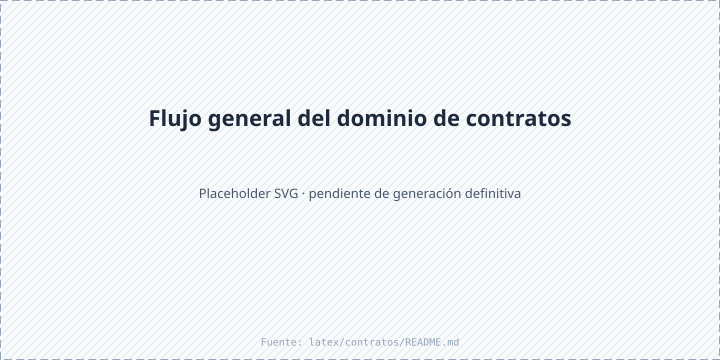
\includegraphics[width=0.95\textwidth]{images/01-flujo-general.svg}}{\fbox{\parbox{0.88\textwidth}{\centering Fallback: contrato $\rightarrow$ prefactura $\rightarrow$ pago validado $\rightarrow$ instalación $\rightarrow$ lecturas/consumo $\rightarrow$ convenios.\\[3pt]Agregar \texttt{images/01-flujo-general.svg} para reemplazar este fallback.}}}
\caption{Flujo general del dominio.}
\end{figure}

\section*{Introducción}
\addcontentsline{toc}{section}{Introducción}
Este documento consolida la documentación técnica de los ocho subdominios que participan en el ciclo de contratos del backend. Describe sus superficies HTTP, casos de uso, estados, persistencia, efectos y aspectos aún pendientes de confirmar. Los diagramas Mermaid de la fuente Markdown se conservan como bloques de código monoespaciado para evitar dependencias de ejecución externas.

\section{Alcance y convenciones}

La documentación distingue tres niveles: \textbf{Confirmada} (visible en código, Prisma, migración o handler registrado), \textbf{Inferida} (deducción que no prueba una escritura o transición) y \textbf{No encontrada} (la revisión no halló fórmula, handler, rollback, transición o integración). Las fórmulas sólo se presentan como vigentes cuando incluyen fuente, símbolo y línea aproximada. Los efectos directos son escrituras del caso de uso/repositorio; los indirectos provienen de handlers, eventos o funciones SQL.

\subsection{Decisión funcional propuesta sobre novedades}
No se agregará un estado persistido \texttt{NOVEDAD} a \texttt{OrdenTrabajo}. La orden permanecerá en \texttt{EN\_PROGRESO} mientras exista una novedad y la UI mostrará una alerta derivada de la relación de novedades activas. \texttt{OrdenTrabajo.estado} representa ejecución operativa; \texttt{NovedadOrdenTrabajo.estado}, análisis de anomalía; y \texttt{Lectura.estado}, captura y validación del dato. \texttt{NOVEDAD} es un indicador derivado, no un valor de enum. La decisión está \textbf{pendiente de implementación}; el backend deberá impedir \texttt{COMPLETADA} si una novedad abierta afecta el resultado, y queda pendiente definir el criterio de bloqueo (\texttt{afectaOrden}, tipo, resolución o regla equivalente).

\subsection{Convenciones técnicas}
La API usa el prefijo \texttt{/api/v1}; los \texttt{BigInt} se serializan como strings; \texttt{deletedAt} representa eliminación lógica; y ``transaccional'' sólo se usa cuando la transacción fue confirmada. La fuente primaria es el código implementado y el esquema Prisma.

\section{Clientes}


Subdominio de identidad y datos del titular. La API usa \texttt{\detokenize{/api/v1}} y autenticación Bearer.


\begin{quote}
\textbf{Ficha de dominio:} documenta el alta, consulta, actualización y baja lógica de clientes, además del catálogo de tipos de identificación. El alcance cubre las superficies HTTP confirmadas en \texttt{\detokenize{ClientController}}.
\end{quote}


\subsection{Alcance y entradas HTTP}


\begin{itemize}
\item \textbf{Controlador:} \texttt{\detokenize{ClientController}} (\texttt{\detokenize{backend/src/operations/clients/interfaces/http/client.controller.ts}}).
\item \textbf{Servicio:} \texttt{\detokenize{ClientService}}.
\item \textbf{Casos:} \texttt{\detokenize{CreateClientUseCase}}, \texttt{\detokenize{FindOneClientUseCase}}, \texttt{\detokenize{UpdateClientUseCase}}, \texttt{\detokenize{RemoveClientUseCase}}.
\item \texttt{\detokenize{GET /identification-types}} no tiene caso de uso dedicado.
\item \texttt{\detokenize{GET /clients}} tampoco tiene \texttt{\detokenize{FindAllClientUseCase}}: el servicio construye filtros y pagina directamente.
\end{itemize}

\subsection{Comportamiento de negocio verificable}
Las tablas relacionadas son \texttt{Clientes} y \texttt{CatalogoTiposIdentificacion}; \texttt{Contratos} consume la identidad del titular. La transición del contrato al completar una instalación (\texttt{detokenize{INSTALACION}}) o reconexión (\texttt{detokenize{RECONEXION}}) \textbf{sí} existe --- está implementada vía \texttt{detokenize{applyContractLifecycleTransition}} (\texttt{backend/src/operations/routes/infrastructure/repositories/prisma-orden-trabajo.repository.ts:356-403}) y documentada en \texttt{02-contratos.md}, sección ``Transiciones de estado del contrato''. El flujo del cliente es alta, actualización, baja lógica y consulta del catálogo; las validaciones de identificación (algoritmo verificador) son ejecutadas en \texttt{detokenize{CreateClientUseCase}} y \texttt{detokenize{UpdateClientUseCase}}.


\begin{center}
\small
\begin{longtable}{|p{0.313\textwidth}|p{0.313\textwidth}|p{0.313\textwidth}|}
\hline
\textbf{Método y ruta} & \textbf{Caso/servicio ejecutado} & \textbf{Resultado} \\
\hline
\endfirsthead
\hline
\textbf{Método y ruta} & \textbf{Caso/servicio ejecutado} & \textbf{Resultado} \\
\hline
\endhead
\texttt{\detokenize{GET /api/v1/clients/identification-types}} & \texttt{\detokenize{ClientService.findAllIdentificaciones()}} & Catálogo activo. \\
\hline
\texttt{\detokenize{POST /api/v1/clients}} & \texttt{\detokenize{ClientService.create()}} → \texttt{\detokenize{CreateClientUseCase.execute()}} & Cliente creado (\texttt{\detokenize{201}}). \\
\hline
\texttt{\detokenize{GET /api/v1/clients}} & \texttt{\detokenize{ClientService.findAll()}} → \texttt{\detokenize{buildClientFilters()}} → \texttt{\detokenize{ClientRepository.paginateClientes()}} & Página de clientes. \\
\hline
\texttt{\detokenize{GET /api/v1/clients/:id}} & \texttt{\detokenize{ClientService.findOne()}} → \texttt{\detokenize{FindOneClientUseCase.execute()}} & Cliente encontrado. \\
\hline
\texttt{\detokenize{PATCH /api/v1/clients/:id}} & \texttt{\detokenize{ClientService.update()}} → \texttt{\detokenize{UpdateClientUseCase.execute()}} & Cliente actualizado. \\
\hline
\texttt{\detokenize{DELETE /api/v1/clients/:id}} & \texttt{\detokenize{ClientService.delete()}} → \texttt{\detokenize{RemoveClientUseCase.execute()}} & Soft delete. \\
\hline
\end{longtable}
\end{center}


\subsection{Ejemplo JSON}


\begin{lstlisting}
{
  "clienteId": "10",
  "identificacion": "1712345678",
  "nombres": "Juan",
  "apellidos": "Pérez",
  "razonSocial": null,
  "email": "juan@example.com",
  "telefono": "0991234567",
  "direccionDomicilio": "Av. Principal 123",
  "activo": true
}
\end{lstlisting}


\begin{center}
\small
\begin{longtable}{|p{0.313\textwidth}|p{0.313\textwidth}|p{0.313\textwidth}|}
\hline
\textbf{Campo} & \textbf{Tipo} & \textbf{Regla/uso} \\
\hline
\endfirsthead
\hline
\textbf{Campo} & \textbf{Tipo} & \textbf{Regla/uso} \\
\hline
\endhead
\texttt{\detokenize{clienteId}} & string & \texttt{\detokenize{BigInt}} serializado. \\
\hline
\texttt{\detokenize{tipoIdentificacionId}} & number & Referencia al catálogo. \\
\hline
\texttt{\detokenize{identificacion}} & string & Identificador del titular. \\
\hline
\texttt{\detokenize{nombres}}, \texttt{\detokenize{apellidos}} & string/null & Nombre personal. \\
\hline
\texttt{\detokenize{razonSocial}} & string/null & Nombre empresarial cuando aplica. \\
\hline
\texttt{\detokenize{email}}, \texttt{\detokenize{telefono}}, \texttt{\detokenize{direccionDomicilio}} & string/null & Datos de contacto y domicilio. \\
\hline
\texttt{\detokenize{activo}} & boolean & Disponibilidad lógica expuesta por el DTO. \\
\hline
\end{longtable}
\end{center}


\subsection{Estados}


No existe enum vigente de estado del cliente. La disponibilidad se expresa con los siguientes campos:

\begin{center}
\small
\begin{longtable}{|p{0.30\textwidth}|p{0.25\textwidth}|p{0.40\textwidth}|}
\hline
\textbf{Campo} & \textbf{Tipo} & \textbf{Significado} \\
\hline
\endfirsthead
\hline
\textbf{Campo} & \textbf{Tipo} & \textbf{Significado} \\
\hline
\endhead
\texttt{\detokenize{activo}} & \texttt{\detokenize{boolean}} & Habilitación lógica expuesta por el DTO. Por defecto \texttt{\detokenize{true}}. \\
\hline
\texttt{\detokenize{deletedAt}} & \texttt{\detokenize{DateTime?}} & Soft delete; \textbf{interno} para el flujo de consulta, pero \textbf{SÍ se expone} en el DTO \texttt{\detokenize{ClientResponseDto}}. Un cliente puede tener \texttt{\detokenize{activo=true}} y \texttt{\detokenize{deletedAt != null}} simultáneamente. \\
\hline
\texttt{\detokenize{aplicaTerceraEdad}} & \texttt{\detokenize{boolean}} & Calculado en create/update según \texttt{\detokenize{TerceraEdadUtil.aplica(fechaNacimiento)}}. Por defecto \texttt{\detokenize{false}}. \\
\hline
\texttt{\detokenize{aplicaDiscapacidad}} & \texttt{\detokenize{boolean}} & Flag configurable desde el DTO. Por defecto \texttt{\detokenize{false}}. \\
\hline
\texttt{\detokenize{telefonoSecundario}} & \texttt{\detokenize{string?}} & Teléfono alternativo. Presente en el modelo y en el DTO. \\
\hline
\texttt{\detokenize{tipoIdentificacion}} & \texttt{\detokenize{CatalogoTiposIdentificacion}} & Relación al catálogo; el enum \texttt{\detokenize{TipoIdentificacion}} tiene 5 valores (\texttt{\detokenize{CEDULA}}, \texttt{\detokenize{RUC}}, \texttt{\detokenize{PASAPORTE}}, \texttt{\detokenize{CONSUMIDOR\\_FINAL}}, \texttt{\detokenize{IDENTIFICACION\\_EXTRANJERA}}). \\
\hline
\end{longtable}
\end{center}

No hay reactivación pública: el flujo \texttt{\detokenize{POST /clients}} reactiva un registro existente solo cuando el \texttt{\detokenize{tipoIdentificacionId=4}} (\texttt{\detokenize{CONSUMIDOR\\_FINAL}}) o cuando la \texttt{\detokenize{identificacion}} ya existía con \texttt{\detokenize{deletedAt != null}}.

\subsubsection{Validación de identificación por algoritmo verificador}

\texttt{\detokenize{CreateClientUseCase}} y \texttt{\detokenize{UpdateClientUseCase}} invocan \texttt{\detokenize{TipoIdentificacionUtil.validar(codigo, identificacion)}} antes de persistir. Las reglas por tipo son:

\begin{center}
\small
\begin{longtable}{|p{0.30\textwidth}|p{0.35\textwidth}|p{0.30\textwidth}|}
\hline
\textbf{\texttt{\detokenize{codigo}} (SRI)} & \textbf{Tipo} & \textbf{Regla} \\
\hline
\endfirsthead
\hline
\textbf{\texttt{\detokenize{codigo}} (SRI)} & \textbf{Tipo} & \textbf{Regla} \\
\hline
\endhead
\texttt{\detokenize{05}} & \texttt{\detokenize{CEDULA}} & 10 dígitos, algoritmo módulo 10. \\
\hline
\texttt{\detokenize{04}} (con terminación \texttt{\detokenize{001}}) & \texttt{\detokenize{RUC persona natural}} & Cédula + \texttt{\detokenize{001}}. \\
\hline
\texttt{\detokenize{04}} (con tercer dígito \texttt{\detokenize{9}}, terminación \texttt{\detokenize{001}}) & \texttt{\detokenize{RUC privado}} & Algoritmo módulo 11 con coeficientes \texttt{\detokenize{[4,3,2,7,6,5,4,3,2]}}. \\
\hline
\texttt{\detokenize{04}} (con tercer dígito \texttt{\detokenize{6}}, terminación \texttt{\detokenize{0001}}) & \texttt{\detokenize{RUC público}} & Algoritmo módulo 11 con coeficientes \texttt{\detokenize{[3,2,7,6,5,4,3,2]}}. \\
\hline
\texttt{\detokenize{08}} & \texttt{\detokenize{PASAPORTE}} & Sin validación de checksum (solo presencia). \\
\hline
\texttt{\detokenize{09}} & \texttt{\detokenize{IDENTIFICACION\\_EXTRANJERA}} & Sin validación de checksum. \\
\hline
\texttt{\detokenize{07}} & \texttt{\detokenize{CONSUMIDOR\\_FINAL}} & No requiere \texttt{\detokenize{identificacion}}; usa lógica de singleton con reactivación (ver más abajo). \\
\hline
\end{longtable}
\end{center}

\begin{quote}
\textbf{Nota cross-doc:} la nota en \texttt{\detokenize{../HISTORIAS-DE-USUARIO.md}}, escenario HU-01, marcaba esta validación como ``pendiente de implementación''. La implementación SÍ existe en \texttt{\detokenize{backend/src/shared/utils/tipo-identificacion.util.ts}}. Esa nota está desactualizada.
\end{quote}

\subsubsection{Singleton CONSUMIDOR FINAL}

El tipo de identificación con \texttt{\detokenize{id=4}} (codigo SRI \texttt{\detokenize{07}}, \texttt{\detokenize{CONSUMIDOR\\_FINAL}}) tiene semántica especial: existe \textbf{a lo sumo un} registro activo de este tipo en toda la tabla.

\begin{itemize}
\item \texttt{\detokenize{CreateClientUseCase}} detecta \texttt{\detokenize{tipoIdentificacionId === 4}} y llama a \texttt{\detokenize{clientRepository.reactivateOrCreateConsumidorFinal(...)}}.
\item Si existe al menos un registro activo o soft-deleted, se reutiliza el más antiguo y se reactivan los datos del request (\texttt{\detokenize{email}}, \texttt{\detokenize{teléfono}}, \texttt{\detokenize{dirección}}).
\item Si hay más de un registro, los extras se marcan con \texttt{\detokenize{deletedAt = now}} para mantener el invariante de singleton.
\end{itemize}

No requiere \texttt{\detokenize{identificacion}} ni \texttt{\detokenize{nombres/apellidos}}.


\subsection{Efectos y transacciones}


Crear, actualizar y eliminar escriben \texttt{\detokenize{Clientes}} mediante sus casos de uso; eliminar usa soft delete. Las consultas, \texttt{\detokenize{buildClientFilters}} y \texttt{\detokenize{ClientResponseDto.fromEntity}} son transformaciones/serialización puras. No se confirmó una transacción adicional ni handler de eventos propio.


\begin{center}
\small
\begin{longtable}{|p{0.470\textwidth}|p{0.470\textwidth}|}
\hline
\textbf{Tabla Prisma} & \textbf{Uso} \\
\hline
\endfirsthead
\hline
\textbf{Tabla Prisma} & \textbf{Uso} \\
\hline
\endhead
\texttt{\detokenize{Clientes}} & Titular y soft delete. \\
\hline
\texttt{\detokenize{CatalogoTiposIdentificacion}} & Tipos activos y relación. \\
\hline
\end{longtable}
\end{center}


\subsection{Gráfico de estados}


\begin{lstlisting}
stateDiagram-v2
  [*] --> Activo: crear
  Activo --> Eliminado: DELETE (soft delete)
\end{lstlisting}


\subsection{Casos de uso}


\subsubsection{Caso: Catálogo de tipos de identificación}


\textbf{Descripción:} devuelve los tipos activos para formularios.


\textbf{HTTP y ruta:} \texttt{\detokenize{GET /api/v1/clients/identification-types}}.


\textbf{Permiso:} \texttt{\detokenize{clientes:read}}.


\textbf{Cadena:} \texttt{\detokenize{ClientController.findAllIdentificaciones()}} → \texttt{\detokenize{ClientService.findAllIdentificaciones()}} → \texttt{\detokenize{ClientRepository.findActiveTipoIdentificaciones()}} (sin caso dedicado).


\textbf{Errores relevantes:} \texttt{\detokenize{401}} no autenticado; \texttt{\detokenize{403}} sin permiso.


\textbf{Efectos:} ninguno; consulta y mapeo puros.


\textbf{Prisma:} \texttt{\detokenize{CatalogoTiposIdentificacion}}.


\textbf{Entrada:} sin body, path ni query.


\textbf{Salida:}


\begin{lstlisting}
[
  {
    "tipoIdentificacionId": 1,
    "codigo": "CEDULA",
    "descripcion": "Cédula"
  }
]
\end{lstlisting}


\subsubsection{Caso: Crear cliente}


\textbf{Descripción:} registra un nuevo titular.


\textbf{HTTP y ruta:} \texttt{\detokenize{POST /api/v1/clients}}.


\textbf{Permiso:} \texttt{\detokenize{clientes:create}}.


\textbf{Cadena:} \texttt{\detokenize{ClientController.create()}} → \texttt{\detokenize{ClientService.create()}} → \texttt{\detokenize{CreateClientUseCase.execute()}} → \texttt{\detokenize{ClientRepository}}.


\textbf{Errores relevantes:}
\begin{itemize}
\item \texttt{\detokenize{400}} datos inválidos (incluye validación del algoritmo verificador según el tipo).
\item \texttt{\detokenize{401}}.
\item \texttt{\detokenize{403}}.
\item \textbf{Conflicto de identificación} (ya activa) --- \texttt{\detokenize{EntityAlreadyExistsException}}.
\item \textbf{Identificación inválida} según el algoritmo --- \texttt{\detokenize{InvalidDomainOperationException}}.
\item \textbf{Campos requeridos faltantes} según el tipo (\texttt{\detokenize{nombres}}/\texttt{\detokenize{apellidos}}/\texttt{\detokenize{direccionDomicilio}} para tipos genéricos; \texttt{\detokenize{razonSocial}} adicional para RUC).
\end{itemize}

\textbf{Efectos:}
\begin{itemize}
\item Alta en \texttt{\detokenize{Clientes}} \textbf{o reactivación} si la identificación existía soft-deleted.
\item Cálculo automático de \texttt{\detokenize{aplicaTerceraEdad}} vía \texttt{\detokenize{TerceraEdadUtil.aplica(fechaNacimiento)}}.
\item Normalización: emails a lowercase, nombres/apellidos/razonSocial a uppercase, identificación con \texttt{\detokenize{trim}}.
\item El DTO de salida es serialización pura.
\end{itemize}


\textbf{Prisma:} \texttt{\detokenize{Clientes}}, \texttt{\detokenize{CatalogoTiposIdentificacion}}.


\textbf{Entrada:}


\begin{lstlisting}
{
  "tipoIdentificacionId": 1,
  "identificacion": "1712345678",
  "nombres": "Juan",
  "apellidos": "Pérez",
  "razonSocial": null,
  "email": "juan@example.com"
}
\end{lstlisting}


\textbf{Salida:}


\begin{lstlisting}
{
  "clienteId": "10",
  "identificacion": "1712345678",
  "nombres": "Juan",
  "apellidos": "Pérez",
  "razonSocial": null,
  "email": "juan@example.com",
  "telefono": null,
  "direccionDomicilio": null,
  "activo": true
}
\end{lstlisting}


\subsubsection{Caso: Listar clientes}


\textbf{Descripción:} consulta clientes con filtros opcionales y paginación.


\textbf{HTTP y ruta:} \texttt{\detokenize{GET /api/v1/clients}}.


\textbf{Permiso:} \texttt{\detokenize{clientes:read}}.


\textbf{Cadena:} \texttt{\detokenize{ClientController.findAll()}} → \texttt{\detokenize{ClientService.findAll()}} → \texttt{\detokenize{buildClientFilters()}} → \texttt{\detokenize{ClientRepository.paginateClientes()}}; no existe \texttt{\detokenize{FindAllClientUseCase}}.


\textbf{Errores relevantes:} \texttt{\detokenize{400}} query inválida; \texttt{\detokenize{401}}; \texttt{\detokenize{403}}.


\textbf{Efectos:} ninguno; consulta y DTO puros.


\textbf{Prisma:} \texttt{\detokenize{Clientes}}, \texttt{\detokenize{CatalogoTiposIdentificacion}}.


\textbf{Entrada:} sin body. Query: \texttt{\detokenize{page}}, \texttt{\detokenize{limit}}, \texttt{\detokenize{identificacion}}, \texttt{\detokenize{nombres}}, \texttt{\detokenize{apellidos}}, \texttt{\detokenize{nombreCompleto}}.


\textbf{Salida:}


\begin{lstlisting}
{
  "data": [
    {
      "clienteId": "10",
      "identificacion": "1712345678",
      "nombres": "Juan",
      "apellidos": "Pérez",
      "activo": true
    }
  ],
  "meta": {
    "page": 1,
    "limit": 10,
    "total": 1,
    "totalPages": 1
  }
}
\end{lstlisting}


\subsubsection{Caso: Obtener cliente}


\textbf{Descripción:} devuelve un cliente por identificador.


\textbf{HTTP y ruta:} \texttt{\detokenize{GET /api/v1/clients/:id}}.


\textbf{Permiso:} \texttt{\detokenize{clientes:read}}.


\textbf{Cadena:} \texttt{\detokenize{ClientController.findOne()}} → \texttt{\detokenize{ClientService.findOne()}} → \texttt{\detokenize{FindOneClientUseCase.execute()}} → \texttt{\detokenize{ClientRepository}}.


\textbf{Errores relevantes:} \texttt{\detokenize{400}} ID inválido; \texttt{\detokenize{401}}; \texttt{\detokenize{403}}; \texttt{\detokenize{404}} no encontrado.


\textbf{Efectos:} ninguno; DTO puro.


\textbf{Prisma:} \texttt{\detokenize{Clientes}}, \texttt{\detokenize{CatalogoTiposIdentificacion}}.


\textbf{Entrada:} sin body. Path: \texttt{\detokenize{{ "id": "10" }}}.


\textbf{Salida:}


\begin{lstlisting}
{
  "clienteId": "10",
  "identificacion": "1712345678",
  "nombres": "Juan",
  "apellidos": "Pérez",
  "razonSocial": null,
  "email": "juan@example.com",
  "telefono": null,
  "direccionDomicilio": null,
  "activo": true
}
\end{lstlisting}


\subsubsection{Caso: Actualizar cliente}


\textbf{Descripción:} modifica parcialmente los datos permitidos del titular.


\textbf{HTTP y ruta:} \texttt{\detokenize{PATCH /api/v1/clients/:id}}.


\textbf{Permiso:} \texttt{\detokenize{clientes:update}}.


\textbf{Cadena:} \texttt{\detokenize{ClientController.update()}} → \texttt{\detokenize{ClientService.update()}} → \texttt{\detokenize{UpdateClientUseCase.execute()}} → \texttt{\detokenize{ClientRepository}}.


\textbf{Errores relevantes:} \texttt{\detokenize{400}} ID/body inválidos; \texttt{\detokenize{401}}; \texttt{\detokenize{403}}; \texttt{\detokenize{404}} no encontrado.


\textbf{Efectos:} actualización de \texttt{\detokenize{Clientes}}; DTO puro.


\textbf{Prisma:} \texttt{\detokenize{Clientes}}, \texttt{\detokenize{CatalogoTiposIdentificacion}}.


\textbf{Entrada:} path \texttt{\detokenize{{ "id": "10" }}}; body:


\begin{lstlisting}
{
  "telefono": "0990000000",
  "email": "nuevo@example.com"
}
\end{lstlisting}


\textbf{Salida:}


\begin{lstlisting}
{
  "clienteId": "10",
  "telefono": "0990000000",
  "email": "nuevo@example.com",
  "activo": true
}
\end{lstlisting}


\subsubsection{Caso: Eliminar cliente}


\textbf{Descripción:} marca el cliente como eliminado sin borrado físico.


\textbf{HTTP y ruta:} \texttt{\detokenize{DELETE /api/v1/clients/:id}}.


\textbf{Permiso:} \texttt{\detokenize{clientes:delete}}.


\textbf{Cadena:} \texttt{\detokenize{ClientController.delete()}} → \texttt{\detokenize{ClientService.delete()}} → \texttt{\detokenize{RemoveClientUseCase.execute()}} → \texttt{\detokenize{ClientRepository}}.


\textbf{Errores relevantes:} \texttt{\detokenize{400}} ID inválido; \texttt{\detokenize{401}}; \texttt{\detokenize{403}}; \texttt{\detokenize{404}} no encontrado.


\textbf{Efectos:} soft delete en \texttt{\detokenize{Clientes}}; \textbf{solo} setea \texttt{\detokenize{deletedAt = now()}} (no toca \texttt{\detokenize{activo}}). Tras la operación, el cliente tiene \texttt{\detokenize{activo=true}} y \texttt{\detokenize{deletedAt != null}} simultáneamente.


\textbf{Prisma:} \texttt{\detokenize{Clientes}}.


\textbf{Entrada:} sin body. Path: \texttt{\detokenize{{ "id": "10" }}}.


\textbf{Salida:} objeto \texttt{\detokenize{ClientResponseDto}} con los 13 campos del DTO, donde \texttt{\detokenize{deletedAt}} está poblado y \texttt{\detokenize{activo}} sigue \texttt{\detokenize{true}}.


\subsection{Pendientes funcionales}

Bloqueos confirmados como pendientes en el código revisado. Cuando se cierre cada uno, sacar de acá y mover a la sección correspondiente.

\begin{itemize}
\item \textbf{Forma exacta de \texttt{\detokenize{CreateClientDto}} y \texttt{\detokenize{UpdateClientDto}}} (campos opcionales vs obligatorios, validaciones anidadas como \texttt{\detokenize{@IsEmail}}, \texttt{\detokenize{@Matches}}). Confirmar contra el código actual; la lista de campos en este doc es funcional, no de validación.
\item \textbf{Forma exacta del query string de \texttt{\detokenize{GET /api/v1/clients}}} (\texttt{\detokenize{page}}, \texttt{\detokenize{limit}}, \texttt{\detokenize{identificacion}}, \texttt{\detokenize{nombres}}, \texttt{\detokenize{apellidos}}, \texttt{\detokenize{nombreCompleto}}). Confirmar que el filtro \texttt{\detokenize{nombreCompleto}} sigue vigente en el repositorio (vista en \texttt{\detokenize{client-filters.mapper.ts}}).
\item \textbf{Reactivación pública de clientes soft-deleted.} Existe \textbf{solo} para \texttt{\detokenize{CONSUMIDOR\\_FINAL}} y como efecto secundario al crear con la misma identificación. No hay endpoint público para reactivar un cliente regular; si se requiere, hay que decidir el criterio (?solo admin?) y agregar el endpoint.
\end{itemize}

\subsection{No documentado o pendiente de confirmar}

\begin{itemize}
\item Handlers de eventos de clientes. No hay event dispatcher que reaccione a cambios en \texttt{\detokenize{Clientes}}. Si se requiere propagar a \texttt{\detokenize{Contratos}} automáticamente (por ejemplo, cambio de dirección), hay que implementar el patrón outbox como en pagos.
\item Estados legacy distintos de \texttt{\detokenize{activo}} y \texttt{\detokenize{deletedAt}}. Confirmar contra seeds y migraciones si existe alguna columna legacy.
\end{itemize}

\section{Contratos}


Vínculo entre cliente, medidor, tarifa y servicio.


\begin{quote}
\textbf{Ficha de dominio:} documenta el ciclo contractual, el vínculo con medidores, la asignación de rutas de instalación, la baja lógica y la generación de documentos PDF.
\end{quote}


\subsection{Alcance y entradas HTTP}


\begin{itemize}
\item \textbf{Controlador:} \texttt{\detokenize{ContratoMedidorController}}.
\item \textbf{Servicio:} \texttt{\detokenize{ContratoMedidorService}}.
\item \textbf{Casos:} \texttt{\detokenize{CreateContractUseCase}}, \texttt{\detokenize{FindAllContractsUseCase}}, \texttt{\detokenize{FindOneContractUseCase}}, \texttt{\detokenize{UpdateContractUseCase}}, \texttt{\detokenize{FinalizeMeterLinkUseCase}}, \texttt{\detokenize{RemoveContractUseCase}}.
\item La asignación de ruta usa el servicio/repositorios; no se confirmó un caso de uso dedicado.
\end{itemize}


\begin{center}
\small
\begin{longtable}{|p{0.313\textwidth}|p{0.313\textwidth}|p{0.313\textwidth}|}
\hline
\textbf{Método y ruta} & \textbf{Caso/servicio ejecutado} & \textbf{Resultado} \\
\hline
\endfirsthead
\hline
\textbf{Método y ruta} & \textbf{Caso/servicio ejecutado} & \textbf{Resultado} \\
\hline
\endhead
\texttt{\detokenize{POST /api/v1/contracts}} & \texttt{\detokenize{crearContrato()}} → \texttt{\detokenize{CreateContractUseCase.execute()}} & Contrato creado. \\
\hline
\texttt{\detokenize{GET /api/v1/contracts}} & \texttt{\detokenize{buscarContratos()}} → \texttt{\detokenize{FindAllContractsUseCase.execute()}} & Página. \\
\hline
\texttt{\detokenize{GET /api/v1/contracts/:id}} & \texttt{\detokenize{buscarContrato()}} → \texttt{\detokenize{FindOneContractUseCase.execute()}} & Detalle. \\
\hline
\texttt{\detokenize{PATCH /api/v1/contracts/:id}} & \texttt{\detokenize{actualizar()}} → \texttt{\detokenize{UpdateContractUseCase.execute()}} & Contrato actualizado. \\
\hline
\texttt{\detokenize{POST /api/v1/contracts/:id/finalize}} & \texttt{\detokenize{finalizarVinculo()}} → \texttt{\detokenize{FinalizeMeterLinkUseCase.execute()}} & Vínculo finalizado. \\
\hline
\texttt{\detokenize{POST /api/v1/contracts/:id/assign-installation-route}} & \texttt{\detokenize{assignInstallationRoute()}} → servicio/repositorios & Ruta y orden de instalación. \\
\hline
\texttt{\detokenize{DELETE /api/v1/contracts/:id}} & \texttt{\detokenize{eliminar()}} → \texttt{\detokenize{RemoveContractUseCase.execute()}} & Soft delete. \\
\hline
\texttt{\detokenize{GET /api/v1/contracts/:id/pdf/connection-request}} & \texttt{\detokenize{generateConnectionRequestPdf()}} & PDF. \\
\hline
\texttt{\detokenize{GET /api/v1/contracts/:id/pdf/responsibility-agreement}} & \texttt{\detokenize{generateResponsibilityAgreementPdf()}} & PDF. \\
\hline
\end{longtable}
\end{center}


\subsection{Ejemplo JSON}


\begin{lstlisting}
{
  "contratoId": "1",
  "clienteId": "10",
  "medidorId": "20",
  "estadoServicio": "PENDIENTE_PAGO",
  "estadoCobranza": "NO_APLICA"
}
\end{lstlisting}


\begin{center}
\small
\begin{longtable}{|p{0.313\textwidth}|p{0.313\textwidth}|p{0.313\textwidth}|}
\hline
\textbf{Campo} & \textbf{Tipo} & \textbf{Regla/uso} \\
\hline
\endfirsthead
\hline
\textbf{Campo} & \textbf{Tipo} & \textbf{Regla/uso} \\
\hline
\endhead
\texttt{\detokenize{contratoId}}, \texttt{\detokenize{clienteId}}, \texttt{\detokenize{medidorId}} & string & \texttt{\detokenize{BigInt}} serializado. \\
\hline
\texttt{\detokenize{categoriaTarifaId}}, \texttt{\detokenize{comunidadId}}, \texttt{\detokenize{sectorId}} & number & Relaciones territoriales/tarifarias. \\
\hline
\texttt{\detokenize{numeroGuia}}, \texttt{\detokenize{direccionSuministro}} & string & Datos de instalación. \\
\hline
\texttt{\detokenize{estadoServicio}} & enum & Ciclo operativo del servicio. \\
\hline
\texttt{\detokenize{estadoCobranza}} & enum & Situación de cobro. \\
\hline
\end{longtable}
\end{center}


\subsection{Estados}


\begin{center}
\small
\begin{longtable}{|p{0.313\textwidth}|p{0.313\textwidth}|p{0.313\textwidth}|}
\hline
\textbf{Dimensión} & \textbf{Valores confirmados} & \textbf{Significado} \\
\hline
\endfirsthead
\hline
\textbf{Dimensión} & \textbf{Valores confirmados} & \textbf{Significado} \\
\hline
\endhead
Servicio & \texttt{\detokenize{PENDIENTE_PAGO}}, \texttt{\detokenize{PENDIENTE_INSTALACION}}, \texttt{\detokenize{ACTIVO}}, \texttt{\detokenize{SUSPENDIDO}}, \texttt{\detokenize{RETIRADO}} & Pago, instalación, operación, suspensión y retiro. \\
\hline
Cobranza & \texttt{\detokenize{NO_APLICA}}, \texttt{\detokenize{AL_DIA}}, \texttt{\detokenize{EN_MORA}} & Sin cobro, corriente o vencido. \\
\hline
\end{longtable}
\end{center}


\subsection{Efectos y transacciones}


La creación valida relaciones y escribe directamente contrato, historial y medidor. La prefactura se obtiene indirectamente mediante \texttt{SELECT generar\_prefactura\_instalacion(...)} dentro de la transacción cuando \texttt{estadoServicio=PENDIENTE\_PAGO}; no se crea directamente desde Prisma.

\subsubsection{Cadena POST y efectos}
La cadena es \texttt{ContratoMedidorController.crear()} $\rightarrow$ \texttt{ContratoMedidorService.crearContrato()} $\rightarrow$ \texttt{CreateContractUseCase.execute()} $\rightarrow$ \texttt{PrismaContractRepository}. Fuentes: \texttt{backend/src/operations/contracts/application/use-cases/create-contract.use-case.ts} (aprox. líneas 30--190), \texttt{backend/src/operations/contracts/infrastructure/repositories/prisma-contract.repository.ts} (aprox. líneas 1--220) y \texttt{backend/src/operations/contracts/interfaces/dto/create-contrato-medidor.dto.ts} (aprox. líneas 1--140). Se validan DTO, cliente, categoría, disponibilidad del medidor y coherencia del estado inicial.

\begin{center}\small
\begin{longtable}{|p{0.28\textwidth}|p{0.18\textwidth}|p{0.48\textwidth}|}
\hline
\textbf{Superficie} & \textbf{Tipo} & \textbf{Efecto} \\
\hline
\texttt{contratos} & Directo & Inserta el vínculo con \texttt{PENDIENTE\_PAGO} y \texttt{NO\_APLICA}. \\
\hline
\texttt{historial\_medidores} & Directo & Registra el vínculo inicial. \\
\hline
\texttt{medidores} & Directo & Reserva/actualiza el estado. \\
\hline
\texttt{Comprobante}, \texttt{ComprobanteDetalle}, \texttt{Prefacturas}, \texttt{PrefacturaDetalle} & Indirecto & Los crea la función SQL dentro de la misma transacción. \\
\hline
\end{longtable}\end{center}

La función está en \texttt{backend/prisma/migrations/20260822010000\_add\_codigo\_sistema\_rubro\_and\_update\_sp/migration.sql} (aprox. líneas 1--260). Selecciona el rubro por categoría y \texttt{codigo\_sistema\_rubro='INSTALACION'}. \texttt{codigo\_sri LIKE 'SERV-GUIA-\%'} es un criterio histórico/legacy, no vigente.

\subsubsection{Fórmula de instalación}
\[
\text{subtotal}=\text{precioUnitario},\quad \text{iva}=\operatorname{ROUND}(\text{subtotal}\times\text{tasaImpuesto},2),\quad \text{total}=\text{subtotal}+\text{iva}.
\]
Fuente: bloque \texttt{generar\_prefactura\_instalacion} de la migración SQL, aprox. líneas 80--220.


\begin{center}
\small
\begin{longtable}{|p{0.470\textwidth}|p{0.470\textwidth}|}
\hline
\textbf{Tabla Prisma} & \textbf{Uso} \\
\hline
\endfirsthead
\hline
\textbf{Tabla Prisma} & \textbf{Uso} \\
\hline
\endhead
\texttt{\detokenize{Contratos}} & Contrato, estados y soft delete. \\
\hline
\texttt{\detokenize{HistorialMedidores}} & Historial del vínculo. \\
\hline
\texttt{\detokenize{Medidores}} & Medidor asociado. \\
\hline
\texttt{\detokenize{CategoriaTarifa}}, \texttt{\detokenize{Clientes}} & Relaciones principales. \\
\hline
\texttt{\detokenize{Prefacturas}}, \texttt{\detokenize{PrefacturaDetalle}}, \texttt{\detokenize{Rubros}} & Cargo de instalación. \\
\hline
\texttt{\detokenize{Rutas}}, \texttt{\detokenize{OrdenTrabajo}} & Instalación asignada. \\
\hline
\end{longtable}
\end{center}


\subsection{Gráfico de estados}


\begin{lstlisting}
stateDiagram-v2
  [*] --> PENDIENTE_PAGO
  PENDIENTE_PAGO --> PENDIENTE_INSTALACION: pago de instalación
  ACTIVO --> SUSPENDIDO
  SUSPENDIDO --> RETIRADO
\end{lstlisting}


\subsection{Casos de uso}


\subsubsection{Caso: Crear contrato}


\textbf{Descripción:} crea el contrato y prepara la instalación del medidor.  

\textbf{HTTP y ruta:} \texttt{\detokenize{POST /api/v1/contracts}}.  

\textbf{Permiso:} \texttt{\detokenize{contracts:create}}.  

\textbf{Cadena:} \texttt{\detokenize{ContratoMedidorController.crear()}} → \texttt{\detokenize{ContratoMedidorService.crearContrato()}} → \texttt{\detokenize{CreateContractUseCase.execute()}} → repositorios.  

\textbf{Errores relevantes:} \texttt{\detokenize{400}} datos/relaciones inválidas; \texttt{\detokenize{401}}; \texttt{\detokenize{403}}; \texttt{\detokenize{404}}; medidor no disponible.  

\textbf{Efectos:} crea contrato, historial y prefactura en las operaciones confirmadas por el caso.  

\textbf{Prisma:} \texttt{\detokenize{Contratos}}, \texttt{\detokenize{HistorialMedidores}}, \texttt{\detokenize{Medidores}}, \texttt{\detokenize{Prefacturas}}, \texttt{\detokenize{PrefacturaDetalle}}, \texttt{\detokenize{Rubros}}, \texttt{\detokenize{Clientes}}, \texttt{\detokenize{CategoriaTarifa}}.  

\textbf{Entrada:}


\begin{lstlisting}
{"clienteId":"10","medidorId":"20","categoriaTarifaId":1,"numeroGuia":"G-0001","direccionSuministro":"Av. Amazonas 123","comunidadId":1}
\end{lstlisting}


\textbf{Salida:}


\begin{lstlisting}
{"contratoId":"1","clienteId":"10","medidorId":"20","estadoServicio":"PENDIENTE_PAGO","estadoCobranza":"NO_APLICA"}
\end{lstlisting}


\subsubsection{Caso: Listar contratos}


\textbf{Descripción:} devuelve contratos filtrados y paginados.  

\textbf{HTTP y ruta:} \texttt{\detokenize{GET /api/v1/contracts}}.  

\textbf{Permiso:} \texttt{\detokenize{contracts:read}}.  

\textbf{Cadena:} \texttt{\detokenize{ContratoMedidorController.buscarContratos()}} → \texttt{\detokenize{ContratoMedidorService.buscarContratos()}} → \texttt{\detokenize{FindAllContractsUseCase.execute()}} → repositorio.  

\textbf{Errores relevantes:} \texttt{\detokenize{400}} query inválida; \texttt{\detokenize{401}}; \texttt{\detokenize{403}}.  

\textbf{Efectos:} ninguno; consulta y DTO puros.  

\textbf{Prisma:} \texttt{\detokenize{Contratos}}, \texttt{\detokenize{Clientes}}, \texttt{\detokenize{Medidores}}, \texttt{\detokenize{CategoriaTarifa}}.  

\textbf{Entrada:} sin body; query del \texttt{\detokenize{FilterContractsDto}} (paginación y filtros definidos por el DTO).  

\textbf{Salida:}


\begin{lstlisting}
{"data":[{"contratoId":"1","estadoServicio":"ACTIVO"}],"meta":{"page":1,"limit":10,"total":1,"totalPages":1}}
\end{lstlisting}


\subsubsection{Caso: Obtener contrato}


\textbf{Descripción:} consulta el detalle de un contrato.  

\textbf{HTTP y ruta:} \texttt{\detokenize{GET /api/v1/contracts/:id}}.  

\textbf{Permiso:} \texttt{\detokenize{contracts:read}}.  

\textbf{Cadena:} \texttt{\detokenize{ContratoMedidorController.buscarContrato()}} → \texttt{\detokenize{ContratoMedidorService.buscarContrato()}} → \texttt{\detokenize{FindOneContractUseCase.execute()}} → repositorio.  

\textbf{Errores relevantes:} \texttt{\detokenize{400}}; \texttt{\detokenize{401}}; \texttt{\detokenize{403}}; \texttt{\detokenize{404}}.  

\textbf{Efectos:} ninguno; mapeo puro.  

\textbf{Prisma:} \texttt{\detokenize{Contratos}}, \texttt{\detokenize{Clientes}}, \texttt{\detokenize{Medidores}}, \texttt{\detokenize{CategoriaTarifa}}, \texttt{\detokenize{HistorialMedidores}}.  

\textbf{Entrada:} sin body; path \texttt{\detokenize{{ "id": "1" }}}.  

\textbf{Salida:}


\begin{lstlisting}
{"contratoId":"1","clienteId":"10","estadoServicio":"ACTIVO","estadoCobranza":"AL_DIA","historialMedidores":[]}
\end{lstlisting}


\subsubsection{Caso: Actualizar contrato}


\textbf{Descripción:} actualiza estados, dirección, sector o reemplaza el medidor si se envía \texttt{\detokenize{medidorId}}.  

\textbf{HTTP y ruta:} \texttt{\detokenize{PATCH /api/v1/contracts/:id}}.  

\textbf{Permiso:} \texttt{\detokenize{contracts:update}}.  

\textbf{Cadena:} \texttt{\detokenize{ContratoMedidorController.actualizarContrato()}} → \texttt{\detokenize{ContratoMedidorService.actualizar()}} → \texttt{\detokenize{UpdateContractUseCase.execute()}} → repositorio.  

\textbf{Errores relevantes:} \texttt{\detokenize{400}}; \texttt{\detokenize{401}}; \texttt{\detokenize{403}}; \texttt{\detokenize{404}}; conflicto de estado/relación.  

\textbf{Efectos:} actualización; el reemplazo indicado se ejecuta transaccionalmente según el caso.  

\textbf{Prisma:} \texttt{\detokenize{Contratos}}, \texttt{\detokenize{Medidores}}, \texttt{\detokenize{HistorialMedidores}}.  

\textbf{Entrada:} path \texttt{\detokenize{{ "id": "1" }}}; body \texttt{\detokenize{{ "direccionSuministro": "Calle Nueva 10" }}}.  

\textbf{Salida:}


\begin{lstlisting}
{"contratoId":"1","direccionSuministro":"Calle Nueva 10","estadoServicio":"ACTIVO"}
\end{lstlisting}


\subsubsection{Caso: Finalizar vínculo de medidor}


\textbf{Descripción:} finaliza el vínculo activo del contrato con su medidor.  

\textbf{HTTP y ruta:} \texttt{\detokenize{POST /api/v1/contracts/:id/finalize}}.  

\textbf{Permiso:} \texttt{\detokenize{contracts:update}}.  

\textbf{Cadena:} \texttt{\detokenize{ContratoMedidorController.finalizarVinculo()}} → \texttt{\detokenize{ContratoMedidorService.finalizarVinculo()}} → \texttt{\detokenize{FinalizeMeterLinkUseCase.execute()}} → repositorio.  

\textbf{Errores relevantes:} \texttt{\detokenize{400}}; \texttt{\detokenize{401}}; \texttt{\detokenize{403}}; \texttt{\detokenize{404}}.  

\textbf{Efectos:} registra el cierre en el historial.  

\textbf{Prisma:} \texttt{\detokenize{HistorialMedidores}}, \texttt{\detokenize{Contratos}}, \texttt{\detokenize{Medidores}}.  

\textbf{Entrada:} sin body; path \texttt{\detokenize{{ "id": "1" }}}.  

\textbf{Salida:}


\begin{lstlisting}
{"contratoId":"1","fechaFin":"2026-09-16"}
\end{lstlisting}


\subsubsection{Caso: Asignar ruta de instalación}


\textbf{Descripción:} asigna un contrato pendiente de instalación a una ruta existente o crea una ruta de instalación y su orden.  

\textbf{HTTP y ruta:} \texttt{\detokenize{POST /api/v1/contracts/:id/assign-installation-route}}.  

\textbf{Permiso:} \texttt{\detokenize{contracts:update}}.  

\textbf{Cadena:} \texttt{\detokenize{ContratoMedidorController.assignInstallationRoute()}} → \texttt{\detokenize{ContratoMedidorService.assignInstallationRoute()}} → repositorios de rutas/órdenes.  

\textbf{Errores relevantes:} \texttt{\detokenize{400}}; \texttt{\detokenize{401}}; \texttt{\detokenize{403}}; \texttt{\detokenize{404}}; ruta destino inválida.  

\textbf{Efectos:} crea/reutiliza \texttt{\detokenize{Rutas}} y crea \texttt{\detokenize{OrdenTrabajo}}; no se confirma atomicidad de ambas escrituras.  

\textbf{Prisma:} \texttt{\detokenize{Rutas}}, \texttt{\detokenize{OrdenTrabajo}}, \texttt{\detokenize{Contratos}}, \texttt{\detokenize{Medidores}}.  

\textbf{Entrada:} path \texttt{\detokenize{{ "id": "1" }}}; body \texttt{\detokenize{{ "routeId": "42" }}} o DTO sin \texttt{\detokenize{routeId}} según el código.  

\textbf{Salida:}


\begin{lstlisting}
{"rutaId":"42","tipoRuta":"INSTALACION","ordenesTrabajo":[{"ordenTrabajoId":"9","estado":"PENDIENTE"}]}
\end{lstlisting}


\subsubsection{Caso: Eliminar contrato}


\textbf{Descripción:} marca el contrato como eliminado lógicamente.  

\textbf{HTTP y ruta:} \texttt{\detokenize{DELETE /api/v1/contracts/:id}}.  

\textbf{Permiso:} \texttt{\detokenize{contracts:delete}}.  

\textbf{Cadena:} \texttt{\detokenize{ContratoMedidorController.eliminarContrato()}} → \texttt{\detokenize{ContratoMedidorService.eliminar()}} → \texttt{\detokenize{RemoveContractUseCase.execute()}} → repositorio.  

\textbf{Errores relevantes:} \texttt{\detokenize{400}}; \texttt{\detokenize{401}}; \texttt{\detokenize{403}}; \texttt{\detokenize{404}}.  

\textbf{Efectos:} soft delete en \texttt{\detokenize{Contratos}}.  

\textbf{Prisma:} \texttt{\detokenize{Contratos}}.  

\textbf{Entrada:} sin body; path \texttt{\detokenize{{ "id": "1" }}}.  

\textbf{Salida:}


\begin{lstlisting}
{"contratoId":"1","estadoServicio":"ACTIVO","estadoCobranza":"AL_DIA"}
\end{lstlisting}


\subsubsection{Caso: Generar PDF de solicitud de conexión}


\textbf{Descripción:} genera la solicitud oficial de conexión.  

\textbf{HTTP y ruta:} \texttt{\detokenize{GET /api/v1/contracts/:id/pdf/connection-request}}.  

\textbf{Permiso:} \texttt{\detokenize{contracts:read}}.  

\textbf{Cadena:} \texttt{\detokenize{ContratoMedidorController.connectionRequestPdf()}} → \texttt{\detokenize{ContratoMedidorService.generateConnectionRequestPdf()}} → \texttt{\detokenize{GetConnectionRequestPdfDataUseCase}} → generador.  

\textbf{Errores relevantes:} \texttt{\detokenize{400}}; \texttt{\detokenize{401}}; \texttt{\detokenize{403}}; \texttt{\detokenize{404}}; aborto de solicitud.  

\textbf{Efectos:} sólo lectura y proyección; serialización PDF pura.  

\textbf{Prisma:} \texttt{\detokenize{Contratos}}, \texttt{\detokenize{Clientes}}, \texttt{\detokenize{Medidores}}, \texttt{\detokenize{CategoriaTarifa}}.  

\textbf{Entrada:} sin body; path \texttt{\detokenize{{ "id": "1" }}}.  

\textbf{Salida:} no es JSON: \texttt{\detokenize{Content-Type: application/pdf}}, \texttt{\detokenize{Content-Disposition: inline}} y \texttt{\detokenize{Content-Length}}, con bytes PDF.


\subsubsection{Caso: Generar PDF de acuerdo de responsabilidad}


\textbf{Descripción:} genera el acta de responsabilidad asociada al contrato.  

\textbf{HTTP y ruta:} \texttt{\detokenize{GET /api/v1/contracts/:id/pdf/responsibility-agreement}}.  

\textbf{Permiso:} \texttt{\detokenize{contracts:read}}.  

\textbf{Cadena:} \texttt{\detokenize{ContratoMedidorController.responsibilityAgreementPdf()}} → \texttt{\detokenize{ContratoMedidorService.generateResponsibilityAgreementPdf()}} → \texttt{\detokenize{GetResponsibilityAgreementPdfDataUseCase}} → generador.  

\textbf{Errores relevantes:} \texttt{\detokenize{400}}; \texttt{\detokenize{401}}; \texttt{\detokenize{403}}; \texttt{\detokenize{404}}; aborto de solicitud.  

\textbf{Efectos:} no se confirma escritura de dominio; proyección y PDF puros.  

\textbf{Prisma:} \texttt{\detokenize{Contratos}}, \texttt{\detokenize{Clientes}}, \texttt{\detokenize{Medidores}}, \texttt{\detokenize{HistorialMedidores}}.  

\textbf{Entrada:} sin body; path \texttt{\detokenize{{ "id": "1" }}}.  

\textbf{Salida:} no es JSON: \texttt{\detokenize{application/pdf}}, \texttt{\detokenize{Content-Disposition: inline}}, \texttt{\detokenize{Content-Length}} y bytes PDF.


\subsection{No documentado o pendiente de confirmar}

\begin{figure}[h]
\centering
\IfFileExists{images/02-contrato-prefactura.png}{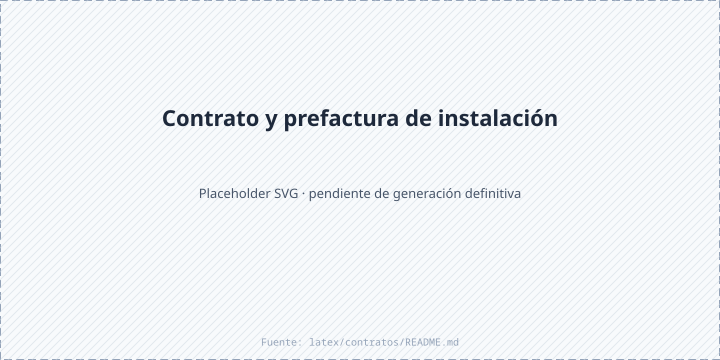
\includegraphics[width=0.9\textwidth]{images/02-contrato-prefactura.png}}{\fbox{\parbox{0.82\textwidth}{\centering Fallback: contrato $\rightarrow$ función SQL $\rightarrow$ comprobante/prefactura. Agregar \texttt{images/02-contrato-prefactura.png} para reemplazarlo.}}}
\caption{Contrato y prefactura de instalación.}
\end{figure}


\begin{itemize}
\item No se encontró transición automática a \texttt{\detokenize{ACTIVO}}. \texttt{PagoValidadoHandler}, en \texttt{backend/src/billing/collections/payments/application/handlers/pago-validado.handler.ts} (aprox. líneas 1--220), confirma \texttt{PENDIENTE\_PAGO} $\rightarrow$ \texttt{PENDIENTE\_INSTALACION} y cobranza \texttt{NO\_APLICA}.
\item Parámetros exactos de los DTO de finalización/asignación si cambian.
\item Sincronización del campo legacy \texttt{\detokenize{estado}}.
\end{itemize}

\section{Convenios de pago}


Financiación de deuda contractual, cuotas y efectos de pagos relacionados.


\begin{quote}
\textbf{Ficha de dominio:} documenta convenios, cuotas, resumen de deuda y pagos relacionados, incluidos sus estados, efectos derivados y superficies de generación de PDF.
\end{quote}


\subsection{Alcance y entradas HTTP}


\begin{itemize}
\item \textbf{Controladores:} \texttt{\detokenize{AgreementsController}} y, para pagos que afectan cuotas, \texttt{\detokenize{PaymentsController}}.
\item \textbf{Servicios:} \texttt{\detokenize{AgreementsService}} y \texttt{\detokenize{PaymentsService}}.
\item \textbf{Casos:} \texttt{\detokenize{GetDebtSummaryUseCase}}, \texttt{\detokenize{CreateAgreementUseCase}}, \texttt{\detokenize{FindOneAgreementUseCase}}, \texttt{\detokenize{UpdateAgreementUseCase}}, \texttt{\detokenize{GetPaymentAgreementPdfDataUseCase}}, \texttt{\detokenize{CreatePaymentUseCase}}, \texttt{\detokenize{ValidatePaymentUseCase}}, \texttt{\detokenize{AnnulPaymentUseCase}}, \texttt{\detokenize{ApplySaldoFavorUseCase}}.
\item Listar convenios y catálogos se resuelven directamente en los servicios; no se confirmó caso dedicado para \texttt{\detokenize{findAll}} ni para catálogos.
\end{itemize}


\begin{center}
\small
\begin{longtable}{|p{0.313\textwidth}|p{0.313\textwidth}|p{0.313\textwidth}|}
\hline
\textbf{Método y ruta} & \textbf{Caso/servicio ejecutado} & \textbf{Resultado} \\
\hline
\endfirsthead
\hline
\textbf{Método y ruta} & \textbf{Caso/servicio ejecutado} & \textbf{Resultado} \\
\hline
\endhead
\texttt{\detokenize{GET /api/v1/agreements/states}} & \texttt{\detokenize{findAllAgreementStates()}} & Estados de convenio. \\
\hline
\texttt{\detokenize{GET /api/v1/agreements/installment-states}} & \texttt{\detokenize{findAllInstallmentStates()}} & Estados de cuota. \\
\hline
\texttt{\detokenize{GET /api/v1/agreements/debt-summary/:contratoId}} & \texttt{\detokenize{getDebtSummary()}} → \texttt{\detokenize{GetDebtSummaryUseCase}} & Deuda. \\
\hline
\texttt{\detokenize{POST /api/v1/agreements}} & \texttt{\detokenize{create()}} → \texttt{\detokenize{CreateAgreementUseCase}} & Convenio y cuotas. \\
\hline
\texttt{\detokenize{GET /api/v1/agreements}} / \texttt{\detokenize{:id}} / \texttt{\detokenize{:id/installments}} & servicio / \texttt{\detokenize{FindOneAgreementUseCase}} & Convenio/cuotas. \\
\hline
\texttt{\detokenize{PATCH /api/v1/agreements/:id}} & \texttt{\detokenize{update()}} → \texttt{\detokenize{UpdateAgreementUseCase}} & Estado. \\
\hline
\texttt{\detokenize{DELETE /api/v1/agreements/:id}} & \texttt{\detokenize{cancel()}} → \texttt{\detokenize{UpdateAgreementUseCase(ANULADO)}} & Anulación. \\
\hline
\texttt{\detokenize{GET /api/v1/agreements/:id/pdf}} & \texttt{\detokenize{generatePdf()}} → \texttt{\detokenize{GetPaymentAgreementPdfDataUseCase}} & PDF. \\
\hline
\texttt{\detokenize{POST/PATCH/DELETE /api/v1/payments...}} & casos de pagos & Crea, valida, aplica o anula pagos. \\
\hline
\end{longtable}
\end{center}


\subsection{Ejemplo JSON}


\begin{lstlisting}
{
  "convenioId": "8",
  "contratoId": "1",
  "deudaTotal": 240.5,
  "abonoInicial": 40,
  "numeroCuotas": 5,
  "estado": "PENDIENTE_ABONO",
  "cuotas": [
    {
      "cuotaConvenioId": "81",
      "numeroCuota": 1,
      "valorCuota": 40.1,
      "estado": "PENDIENTE"
    }
  ]
}
\end{lstlisting}


\begin{center}
\small
\begin{longtable}{|p{0.313\textwidth}|p{0.313\textwidth}|p{0.313\textwidth}|}
\hline
\textbf{Campo} & \textbf{Tipo} & \textbf{Regla/uso} \\
\hline
\endfirsthead
\hline
\textbf{Campo} & \textbf{Tipo} & \textbf{Regla/uso} \\
\hline
\endhead
\texttt{\detokenize{convenioId}}, \texttt{\detokenize{contratoId}}, \texttt{\detokenize{cuotaConvenioId}} & string & \texttt{\detokenize{BigInt}} serializado. \\
\hline
\texttt{\detokenize{deudaTotal}}, \texttt{\detokenize{abonoInicial}}, \texttt{\detokenize{valorCuota}} & number & Valores monetarios. \\
\hline
\texttt{\detokenize{numeroCuotas}}, \texttt{\detokenize{numeroCuota}} & number & Plan y posición. \\
\hline
\texttt{\detokenize{estado}} & enum & Estado de convenio o cuota según el objeto. \\
\hline
\end{longtable}
\end{center}


\subsection{Estados}


\begin{center}
\small
\begin{longtable}{|p{0.313\textwidth}|p{0.313\textwidth}|p{0.313\textwidth}|}
\hline
\textbf{Entidad} & \textbf{Estados} & \textbf{Significado} \\
\hline
\endfirsthead
\hline
\textbf{Entidad} & \textbf{Estados} & \textbf{Significado} \\
\hline
\endhead
Convenio & \texttt{\detokenize{PREPARADO}}, \texttt{\detokenize{PENDIENTE_ABONO}}, \texttt{\detokenize{ACTIVO}}, \texttt{\detokenize{PAGADO}}, \texttt{\detokenize{ANULADO}} & Creado, abono pendiente, vigente, liquidado o anulado. \\
\hline
Cuota & \texttt{\detokenize{PENDIENTE}}, \texttt{\detokenize{PAGADA}} & No liquidada o liquidada. \\
\hline
Pago relacionado & \texttt{\detokenize{PENDIENTE}}, \texttt{\detokenize{REGISTRADO}}, \texttt{\detokenize{ANULADO}} & Por validar, validado o anulado. \\
\hline
\end{longtable}
\end{center}


\subsection{Efectos y transacciones}


Crear convenio calcula deuda y cuotas y persiste \texttt{\detokenize{Convenios}}/\texttt{\detokenize{CuotaConvenio}} en transacción. \texttt{PagoValidadoHandler} actualiza prefacturas y contratos de instalación; \texttt{CuotaPagadaHandler} verifica cuotas y dispara emisión SRI. \texttt{PagoAnuladoHandler} emite nota de crédito si corresponde; no se confirmó rollback de cuotas, prefacturas o contratos. La generación de catálogos, consultas y DTO es pura.

\subsubsection{Tablas y fórmulas confirmadas}
La relación es \texttt{Contratos $\rightarrow$ Convenios $\rightarrow$ CuotaConvenio $\rightarrow$ PrefacturaDetalle $\rightarrow$ Prefacturas}. La deuda usa prefacturas no eliminadas en estados \texttt{GENERADA}, \texttt{EN\_REVISION} o \texttt{APROBADA}:
\[
\text{saldoPrefactura}=\max(0,\text{totalPagar}-\text{abono}),\quad
\text{deudaTotal}=\operatorname{ROUND\_HALF\_UP}(\sum\text{saldoPrefactura},2).
\]
\texttt{mesesMoraActual} cuenta saldos positivos y \texttt{deudaAnterior} busca el período inmediatamente anterior; la continuidad de períodos es una limitación. Fuentes: \texttt{backend/src/billing/collections/agreements/application/use-cases/get-debt-summary.use-case.ts}, \texttt{prisma-agreement-repository.ts} y \texttt{backend/src/shared/utils/debt-calculator.util.ts}.

La tasa se normaliza como \texttt{tasaMensual=tasa/100}; el interés lineal es
\[
\text{interés}=(\text{deudaTotal}-\text{abonoInicial})\times\text{tasaMensual}\times\text{numeroCuotas},\quad
\text{totalADistribuir}=\text{deudaTotal}-\text{abonoInicial}+\text{interés}.
\]
La cuota base es \texttt{TRUNC(totalADistribuir/numeroCuotas,2)} y la última absorbe el residuo. \texttt{CreateAgreementUseCase} (aprox. líneas 30--220) valida deuda, abono, cuotas, tasa y transiciones en transacción. El vencimiento es mensual desde la fecha base.


\begin{center}
\small
\begin{longtable}{|p{0.470\textwidth}|p{0.470\textwidth}|}
\hline
\textbf{Tabla Prisma} & \textbf{Uso} \\
\hline
\endfirsthead
\hline
\textbf{Tabla Prisma} & \textbf{Uso} \\
\hline
\endhead
\texttt{\detokenize{Convenios}} & Plan y estado. \\
\hline
\texttt{\detokenize{CuotaConvenio}} & Cuotas y pagos aplicados. \\
\hline
\texttt{\detokenize{Contratos}}, \texttt{\detokenize{Prefacturas}}, \texttt{\detokenize{PrefacturaDetalle}}, \texttt{\detokenize{Rubros}} & Deuda de origen. \\
\hline
\texttt{\detokenize{Pagos}}, \texttt{\detokenize{DetallePago}}, \texttt{\detokenize{SaldoFavor}} & Cobros y saldos. \\
\hline
\end{longtable}
\end{center}


\subsection{Gráfico de estados}


\begin{lstlisting}
stateDiagram-v2
  [*] --> PREPARADO
  PREPARADO --> PENDIENTE_ABONO
  PENDIENTE_ABONO --> ACTIVO: abono validado
  ACTIVO --> PAGADO: cuotas liquidadas
  ACTIVO --> ANULADO
\end{lstlisting}


\subsection{Casos de uso}


\subsubsection{Caso: Consultar estados de convenio}


\textbf{Descripción:} entrega el catálogo de estados disponibles para convenios.  

\textbf{HTTP y ruta:} \texttt{\detokenize{GET /api/v1/agreements/states}}.  

\textbf{Permiso:} \texttt{\detokenize{agreements:read}}.  

\textbf{Cadena:} \texttt{\detokenize{AgreementsController.findAllStates()}} → \texttt{\detokenize{AgreementsService.findAllAgreementStates()}} → enum.  

\textbf{Errores relevantes:} \texttt{\detokenize{401}}; \texttt{\detokenize{403}}.  

\textbf{Efectos:} ninguno; catálogo de lectura.  

\textbf{Prisma:} ninguna tabla.  

\textbf{Entrada:} sin body, path ni query.  

\textbf{Salida:} \texttt{\detokenize{[ { "codigo": "ACTIVO", "descripcion": "Activo" } ]}}.


\subsubsection{Caso: Consultar estados de cuota}


\textbf{Descripción:} entrega el catálogo de estados disponibles para cuotas.  

\textbf{HTTP y ruta:} \texttt{\detokenize{GET /api/v1/agreements/installment-states}}.  

\textbf{Permiso:} \texttt{\detokenize{agreements:read}}.  

\textbf{Cadena:} \texttt{\detokenize{AgreementsController.findAllInstallmentStates()}} → \texttt{\detokenize{AgreementsService.findAllInstallmentStates()}} → enum.  

\textbf{Errores relevantes:} \texttt{\detokenize{401}}; \texttt{\detokenize{403}}.  

\textbf{Efectos:} ninguno; catálogo de lectura.  

\textbf{Prisma:} ninguna tabla.  

\textbf{Entrada:} sin body, path ni query.  

\textbf{Salida:} \texttt{\detokenize{[ { "codigo": "PENDIENTE", "descripcion": "Pendiente" } ]}}.


\subsubsection{Caso: Consultar resumen de deuda}


\textbf{Descripción:} calcula el resumen de deuda pendiente y devuelve el detalle de las prefacturas impagadas. No expone un total agregado \texttt{montoPagado} en este caso de uso.  

\textbf{HTTP y ruta:} \texttt{\detokenize{GET /api/v1/agreements/debt-summary/:contratoId}}.  

\textbf{Permiso:} \texttt{\detokenize{agreements:read}}.  

\textbf{Cadena:} \texttt{\detokenize{AgreementsController.getDebtSummary()}} → \texttt{\detokenize{AgreementsService.getDebtSummary()}} → \texttt{\detokenize{GetDebtSummaryUseCase.execute()}} → repositorio.  

\textbf{Errores relevantes:} \texttt{\detokenize{400}}; \texttt{\detokenize{401}}; \texttt{\detokenize{403}}; \texttt{\detokenize{404}}.  

\textbf{Efectos:} ninguno.  

\textbf{Prisma:} \texttt{\detokenize{Contratos}}, \texttt{\detokenize{Prefacturas}}, \texttt{\detokenize{PrefacturaDetalle}}, \texttt{\detokenize{Rubros}}, pagos.  

\textbf{Entrada:} sin body; path \texttt{\detokenize{{ "contratoId": "1" }}}.  

\textbf{Salida:} \texttt{\detokenize{{ "contratoId": "1", "deudaTotal": 240.5, "deudaAnterior": 40, "tasaMensualVigente": 2.5, "maxMesesAtrasado": 2, "totalPrefacturasImpagadas": 3, "prefacturas": [] }}}.


\subsubsection{Caso: Crear convenio}


\textbf{Descripción:} crea un plan de pago y genera sus cuotas.  

\textbf{HTTP y ruta:} \texttt{\detokenize{POST /api/v1/agreements}}.  

\textbf{Permiso:} \texttt{\detokenize{agreements:create}}.  

\textbf{Cadena:} \texttt{\detokenize{AgreementsController.create()}} → \texttt{\detokenize{AgreementsService.create()}} → \texttt{\detokenize{CreateAgreementUseCase.execute()}} → repositorio.  

\textbf{Errores relevantes:} \texttt{\detokenize{400}}; \texttt{\detokenize{401}}; \texttt{\detokenize{403}}; \texttt{\detokenize{404}}; deuda no convenible.  

\textbf{Efectos:} persiste convenio y cuotas; no activa por sí solo el contrato.  

\textbf{Prisma:} \texttt{\detokenize{Convenios}}, \texttt{\detokenize{CuotaConvenio}}, \texttt{\detokenize{Contratos}}, prefacturas/rubros.  

\textbf{Entrada:} \texttt{\detokenize{{ "contratoId": "1", "abonoInicial": 40, "numeroCuotas": 5 }}}.  

\textbf{Salida:} JSON del ejemplo principal.


\subsubsection{Caso: Listar convenios}


\textbf{Descripción:} lista convenios paginados y filtrables.  

\textbf{HTTP y ruta:} \texttt{\detokenize{GET /api/v1/agreements}}.  

\textbf{Permiso:} \texttt{\detokenize{agreements:read}}.  

\textbf{Cadena:} \texttt{\detokenize{AgreementsController.findAll()}} → \texttt{\detokenize{AgreementsService.findAll()}} → repositorio; sin caso dedicado confirmado.  

\textbf{Errores relevantes:} \texttt{\detokenize{400}}; \texttt{\detokenize{401}}; \texttt{\detokenize{403}}.  

\textbf{Efectos:} ninguno.  

\textbf{Prisma:} \texttt{\detokenize{Convenios}}, contrato/cliente.  

\textbf{Entrada:} sin body; query \texttt{\detokenize{page}}, \texttt{\detokenize{limit}}, \texttt{\detokenize{contratoId}}, \texttt{\detokenize{estado}}, \texttt{\detokenize{search}}.  

\textbf{Salida:} \texttt{\detokenize{{ "data": [{ "convenioId": "8", "estado": "ACTIVO" }], "meta": {} }}}.


\subsubsection{Caso: Obtener convenio}


\textbf{Descripción:} devuelve el detalle de un convenio por identificador.  

\textbf{HTTP y ruta:} \texttt{\detokenize{GET /api/v1/agreements/:id}}.  

\textbf{Permiso:} \texttt{\detokenize{agreements:read}}.  

\textbf{Cadena:} \texttt{\detokenize{AgreementsController.findOne()}} → \texttt{\detokenize{AgreementsService.findOne()}} → \texttt{\detokenize{FindOneAgreementUseCase.execute()}} → repositorio.  

\textbf{Errores relevantes:} \texttt{\detokenize{400}}; \texttt{\detokenize{401}}; \texttt{\detokenize{403}}; \texttt{\detokenize{404}}.  

\textbf{Efectos:} ninguno; consulta y DTO puros.  

\textbf{Prisma:} \texttt{\detokenize{Convenios}}, \texttt{\detokenize{Contratos}}, \texttt{\detokenize{Clientes}}, \texttt{\detokenize{CuotaConvenio}}.  

\textbf{Entrada:} sin body; path \texttt{\detokenize{{ "id": "8" }}}.  

\textbf{Salida:} objeto JSON \texttt{\detokenize{AgreementResponseDto}} con sus datos y cuotas.


\subsubsection{Caso: Listar cuotas de un convenio}


\textbf{Descripción:} devuelve las cuotas asociadas a un convenio.  

\textbf{HTTP y ruta:} \texttt{\detokenize{GET /api/v1/agreements/:id/installments}}.  

\textbf{Permiso:} \texttt{\detokenize{agreements:read}}.  

\textbf{Cadena:} \texttt{\detokenize{AgreementsController.findInstallments()}} → \texttt{\detokenize{AgreementsService.findInstallments()}} → repositorio.  

\textbf{Errores relevantes:} \texttt{\detokenize{400}}; \texttt{\detokenize{401}}; \texttt{\detokenize{403}}; \texttt{\detokenize{404}}.  

\textbf{Efectos:} ninguno; consulta y DTO puros.  

\textbf{Prisma:} \texttt{\detokenize{CuotaConvenio}}, \texttt{\detokenize{Convenios}}.  

\textbf{Entrada:} sin body; path \texttt{\detokenize{{ "id": "8" }}}.  

\textbf{Salida:} lista JSON \texttt{\detokenize{[ { "cuotaConvenioId": "81", "numeroCuota": 1, "estado": "PENDIENTE" } ]}}.


\subsubsection{Caso: Actualizar estado del convenio}


\textbf{Descripción:} aprueba, paga o cambia el estado permitido del convenio.  

\textbf{HTTP y ruta:} \texttt{\detokenize{PATCH /api/v1/agreements/:id}}.  

\textbf{Permiso:} \texttt{\detokenize{agreements:update}}.  

\textbf{Cadena:} \texttt{\detokenize{AgreementsController.update()}} → \texttt{\detokenize{AgreementsService.update()}} → \texttt{\detokenize{UpdateAgreementUseCase.execute()}} → repositorio.  

\textbf{Errores relevantes:} \texttt{\detokenize{400}}; \texttt{\detokenize{401}}; \texttt{\detokenize{403}}; \texttt{\detokenize{404}}; transición inválida.  

\textbf{Efectos:} \texttt{\detokenize{PAGADO}} puede marcar convenio y cuotas.  

\textbf{Prisma:} \texttt{\detokenize{Convenios}}, \texttt{\detokenize{CuotaConvenio}}.  

\textbf{Entrada:} path \texttt{\detokenize{{ "id": "8" }}}; body \texttt{\detokenize{{ "estado": "ACTIVO" }}}.  

\textbf{Salida:} \texttt{\detokenize{{ "convenioId": "8", "estado": "ACTIVO" }}}.


\subsubsection{Caso: Anular convenio}


\textbf{Descripción:} marca un convenio como \texttt{\detokenize{ANULADO}}.  

\textbf{HTTP y ruta:} \texttt{\detokenize{DELETE /api/v1/agreements/:id}}.  

\textbf{Permiso:} \texttt{\detokenize{agreements:delete}}.  

\textbf{Cadena:} \texttt{\detokenize{AgreementsController.cancel()}} → \texttt{\detokenize{AgreementsService.cancel()}} → \texttt{\detokenize{UpdateAgreementUseCase(ANULADO)}}.  

\textbf{Errores relevantes:} \texttt{\detokenize{400}}; \texttt{\detokenize{401}}; \texttt{\detokenize{403}}; \texttt{\detokenize{404}}.  

\textbf{Efectos:} persiste anulación; no se confirma borrado físico.  

\textbf{Prisma:} \texttt{\detokenize{Convenios}}, cuotas si la transición las afecta.  

\textbf{Entrada:} sin body; path \texttt{\detokenize{{ "id": "8" }}}.  

\textbf{Salida:} \texttt{\detokenize{{ "convenioId": "8", "estado": "ANULADO" }}}.


\subsubsection{Caso: Generar PDF del convenio}


\textbf{Descripción:} genera el documento imprimible del plan.  

\textbf{HTTP y ruta:} \texttt{\detokenize{GET /api/v1/agreements/:id/pdf}}.  

\textbf{Permiso:} \texttt{\detokenize{agreements:read}}.  

\textbf{Cadena:} \texttt{\detokenize{AgreementsController.generatePdf()}} → \texttt{\detokenize{AgreementsService.generatePdf()}} → \texttt{\detokenize{GetPaymentAgreementPdfDataUseCase.execute()}} → dispatcher.  

\textbf{Errores relevantes:} \texttt{\detokenize{400}}; \texttt{\detokenize{401}}; \texttt{\detokenize{403}}; \texttt{\detokenize{404}}; aborto de solicitud.  

\textbf{Efectos:} sólo lectura y proyección; PDF puro.  

\textbf{Prisma:} \texttt{\detokenize{Convenios}}, \texttt{\detokenize{CuotaConvenio}}, \texttt{\detokenize{Contratos}}, \texttt{\detokenize{Clientes}}.  

\textbf{Entrada:} sin body; path \texttt{\detokenize{{ "id": "8" }}}.  

\textbf{Salida:} no es JSON: \texttt{\detokenize{application/pdf}}, \texttt{\detokenize{Content-Disposition: inline}}, \texttt{\detokenize{Content-Length}} y bytes PDF.


\subsection{No documentado o pendiente de confirmar}

\begin{figure}[h]
\centering
\IfFileExists{images/03-convenio-pago.png}{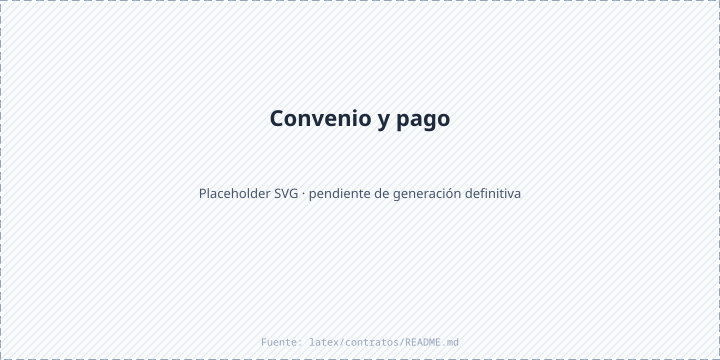
\includegraphics[width=0.9\textwidth]{images/03-convenio-pago.png}}{\fbox{\parbox{0.82\textwidth}{\centering Fallback: deuda $\rightarrow$ convenio $\rightarrow$ cuotas $\rightarrow$ pago. Agregar \texttt{images/03-convenio-pago.png} para reemplazarlo.}}}
\caption{Convenio y pago.}
\end{figure}


\begin{itemize}
\item No se encontró una política completa de mora ni una transición automática adicional fuera de los handlers documentados.
\item El registro de handlers está en \texttt{backend/src/billing/collections/payments/payments.module.ts} (aprox. líneas 1--180).
\item Umbral que convierte una cuota vencida en causal automática de corte.
\end{itemize}

\section{Rutas y órdenes de trabajo}


Despacho de lecturas, instalaciones y operación de campo.


\begin{quote}
\textbf{Ficha de dominio:} documenta períodos, rutas, órdenes de trabajo y operaciones del personal de campo, incluida la vinculación de lecturas y la evidencia externa.
\end{quote}


\subsection{Alcance y entradas HTTP}


\begin{itemize}
\item \textbf{Controladores:} \texttt{\detokenize{RoutesController}}, \texttt{\detokenize{OrdenesTrabajoController}}, \texttt{\detokenize{OperatorController}}.
\item \textbf{Servicios:} \texttt{\detokenize{RoutesService}}, \texttt{\detokenize{OrdenesTrabajoService}}.
\item \textbf{Casos:} \texttt{\detokenize{CreateRouteUseCase}}, \texttt{\detokenize{FindAllRoutesUseCase}}, \texttt{\detokenize{FindOneRouteUseCase}}, \texttt{\detokenize{UpdateRouteUseCase}}, \texttt{\detokenize{DeleteRouteUseCase}}, \texttt{\detokenize{ReassignRouteUseCase}}, \texttt{\detokenize{GetEligibleReadingsUseCase}}, \texttt{\detokenize{GetReadingsByRutaUseCase}}, \texttt{\detokenize{FindOrdenesByRutaUseCase}}, \texttt{\detokenize{ExportFieldSheetPdfUseCase}}, \texttt{\detokenize{UpdateOrdenEstadoUseCase}}, \texttt{\detokenize{LinkLecturaUseCase}}, \texttt{\detokenize{GetOperatorRoutesUseCase}}, \texttt{\detokenize{UpdateRouteStateUseCase}}, \texttt{\detokenize{UpdateOperatorWorkOrderUseCase}}.
\item Los períodos se consultan directamente desde \texttt{\detokenize{RoutesService}}; no se confirmó caso dedicado para listar rutas administrativas ni para algunos cambios de órdenes.
\end{itemize}

\subsection{Comportamiento de negocio verificable}
Las tablas relacionadas son \texttt{Rutas}, \texttt{OrdenTrabajo}, \texttt{EjecucionOrdenTrabajo}, \texttt{Lecturas}, \texttt{Periodos} y \texttt{NovedadOrdenTrabajo}. El flujo confirmado es período $\rightarrow$ ruta $\rightarrow$ orden $\rightarrow$ lectura/evidencia $\rightarrow$ cierre. No se encontró fórmula monetaria que aplique a este módulo. La promoción automática del contrato a \texttt{ACTIVO} al completar orden de instalación \textbf{sí} está implementada --- ver \texttt{02-contratos.md}, sección ``Transiciones de estado del contrato''.


\begin{center}
\small
\begin{longtable}{|p{0.313\textwidth}|p{0.313\textwidth}|p{0.313\textwidth}|}
\hline
\textbf{Método y ruta} & \textbf{Caso/servicio ejecutado} & \textbf{Resultado} \\
\hline
\endfirsthead
\hline
\textbf{Método y ruta} & \textbf{Caso/servicio ejecutado} & \textbf{Resultado} \\
\hline
\endhead
\texttt{\detokenize{GET /api/v1/routes/periods}} & \texttt{\detokenize{RoutesService.getPeriodos()}} & Períodos. \\
\hline
\texttt{\detokenize{GET /api/v1/routes/eligible-readings}} & \texttt{\detokenize{getEligibleReadings()}} → \texttt{\detokenize{GetEligibleReadingsUseCase}} & Lecturas elegibles paginadas. \\
\hline
\texttt{\detokenize{GET /api/v1/routes/:rutaId/readings}} & \texttt{\detokenize{getReadingsByRuta()}} → \texttt{\detokenize{GetReadingsByRutaUseCase}} & Lecturas de ruta. \\
\hline
\texttt{\detokenize{POST /api/v1/routes}} & \texttt{\detokenize{create()}} → \texttt{\detokenize{CreateRouteUseCase}} & Ruta creada. \\
\hline
\texttt{\detokenize{GET /api/v1/routes}} / \texttt{\detokenize{:id}} & \texttt{\detokenize{findAll()}} / \texttt{\detokenize{findOne()}} → casos de consulta & Rutas. \\
\hline
\texttt{\detokenize{PATCH /api/v1/routes/:id}} & \texttt{\detokenize{update()}} → \texttt{\detokenize{UpdateRouteUseCase}} & Ruta actualizada. \\
\hline
\texttt{\detokenize{PATCH /api/v1/routes/:id/reassign}} & \texttt{\detokenize{ReassignRouteUseCase.execute()}} & Operario reasignado. \\
\hline
\texttt{\detokenize{DELETE /api/v1/routes/:id}} & \texttt{\detokenize{delete()}} → \texttt{\detokenize{DeleteRouteUseCase}} & Soft delete. \\
\hline
\texttt{\detokenize{GET /api/v1/routes/:id/pdf}} & \texttt{\detokenize{ExportFieldSheetPdfUseCase}} & PDF. \\
\hline
\texttt{\detokenize{GET /api/v1/routes/:id/work-orders}} & \texttt{\detokenize{FindOrdenesByRutaUseCase}} & Órdenes paginadas. \\
\hline
\texttt{\detokenize{PATCH /api/v1/work-orders/:id/state}} & \texttt{\detokenize{UpdateOrdenEstadoUseCase}} & Estado de orden. \\
\hline
\texttt{\detokenize{PATCH /api/v1/work-orders/:id/reading}} & \texttt{\detokenize{LinkLecturaUseCase}} & Lectura vinculada. \\
\hline
\texttt{\detokenize{GET/PATCH /api/v1/operator/routes...}} & \texttt{\detokenize{GetOperatorRoutesUseCase}} / \texttt{\detokenize{UpdateRouteStateUseCase}} & Vista y estado del operador. \\
\hline
\texttt{\detokenize{PATCH /api/v1/operator/work-orders/:id}} & \texttt{\detokenize{UpdateOperatorWorkOrderUseCase}} & Ejecución/evidencia. \\
\hline
\end{longtable}
\end{center}


\subsection{Ejemplo JSON}


\begin{lstlisting}
{
  "rutaId": "42",
  "nombre": "Lecturas agosto",
  "tipoRuta": "LECTURA",
  "estado": "PENDIENTE",
  "ordenesTrabajo": []
}
\end{lstlisting}


\begin{center}
\small
\begin{longtable}{|p{0.313\textwidth}|p{0.313\textwidth}|p{0.313\textwidth}|}
\hline
\textbf{Campo} & \textbf{Tipo} & \textbf{Regla/uso} \\
\hline
\endfirsthead
\hline
\textbf{Campo} & \textbf{Tipo} & \textbf{Regla/uso} \\
\hline
\endhead
\texttt{\detokenize{rutaId}}, \texttt{\detokenize{ordenTrabajoId}}, \texttt{\detokenize{lecturaId}} & string & \texttt{\detokenize{BigInt}} serializado. \\
\hline
\texttt{\detokenize{tipoRuta}} & enum & Actividad de la ruta. \\
\hline
\texttt{\detokenize{estado}} & enum & Estado de ruta u orden según el DTO. \\
\hline
\texttt{\detokenize{operarioId}}, \texttt{\detokenize{periodoId}}, \texttt{\detokenize{comunidadId}} & number/null & Asignación y contexto. \\
\hline
\texttt{\detokenize{ordenesTrabajo}} & array & Órdenes asociadas. \\
\hline
\end{longtable}
\end{center}


\subsection{Estados}


\begin{center}
\small
\begin{longtable}{|p{0.313\textwidth}|p{0.313\textwidth}|p{0.313\textwidth}|}
\hline
\textbf{Entidad} & \textbf{Estados confirmados} & \textbf{Significado} \\
\hline
\endfirsthead
\hline
\textbf{Entidad} & \textbf{Estados confirmados} & \textbf{Significado} \\
\hline
\endhead
Ruta & \texttt{\detokenize{PENDIENTE}}, \texttt{\detokenize{EN_PROGRESO}}, \texttt{\detokenize{COMPLETADA}}, \texttt{\detokenize{PARCIAL}}, \texttt{\detokenize{CANCELADA}} & Pendiente, ejecutada, finalizada, incompleta o cancelada. \\
\hline
Orden & \texttt{\detokenize{PENDIENTE}}, \texttt{\detokenize{EN_PROGRESO}}, \texttt{\detokenize{COMPLETADA}}, \texttt{\detokenize{CANCELADA}}, \texttt{\detokenize{FALLIDA}} & Ciclo de trabajo. \\
\hline
\end{longtable}
\end{center}

\subsubsection{Máquina de estados de la Ruta}

La máquina está implementada como una tabla de transiciones explícita en \texttt{backend/src/operations/routes/domain/route-state.ts}:

\begin{center}
\small
\begin{longtable}{|p{0.30\textwidth}|p{0.65\textwidth}|}
\hline
\textbf{Desde} & \textbf{Hacia permitidas} \\
\hline
\endfirsthead
\hline
\textbf{Desde} & \textbf{Hacia permitidas} \\
\hline
\endhead
\texttt{\detokenize{PENDIENTE}} & \texttt{\detokenize{EN_PROGRESO}}, \texttt{\detokenize{CANCELADA}} \\
\hline
\texttt{\detokenize{EN_PROGRESO}} & \texttt{\detokenize{COMPLETADA}}, \texttt{\detokenize{PARCIAL}}, \texttt{\detokenize{PENDIENTE}}, \texttt{\detokenize{CANCELADA}} \\
\hline
\texttt{\detokenize{COMPLETADA}} & \texttt{\detokenize{EN_PROGRESO}} (reabre para corrección de cierre) \\
\hline
\texttt{\detokenize{PARCIAL}} & \texttt{\detokenize{EN_PROGRESO}} (reabre para continuar trabajo) \\
\hline
\texttt{\detokenize{CANCELADA}} & \texttt{\detokenize{PENDIENTE}} (reabre para reactivación) \\
\hline
\end{longtable}
\end{center}

La función \texttt{canTransitionRouteState(from, to)} valida la transición; \texttt{UpdateRouteUseCase.execute()} rechaza con \texttt{InvalidDomainOperationException} si la transición no está permitida. \textbf{No existe máquina equivalente para OrdenTrabajo} --- sus transiciones las acepta todas \texttt{UpdateOrdenEstadoUseCase} mientras el estado pertenezca al enum.


\subsection{Regla de novedades sin estado adicional de orden}

\textbf{Decisión funcional propuesta — pendiente de implementación.} No se agregará un estado persistido \texttt{NOVEDAD} a \texttt{OrdenTrabajo}. Mientras exista una novedad, la orden permanece en \texttt{EN\_PROGRESO}; la interfaz muestra una alerta derivada al consultar la relación de novedades activas.

\subsubsection{Flujo acordado de orden con novedad}

\begin{figure}[h]
\centering
\IfFileExists{images/04-orden-lectura-flujo.png}{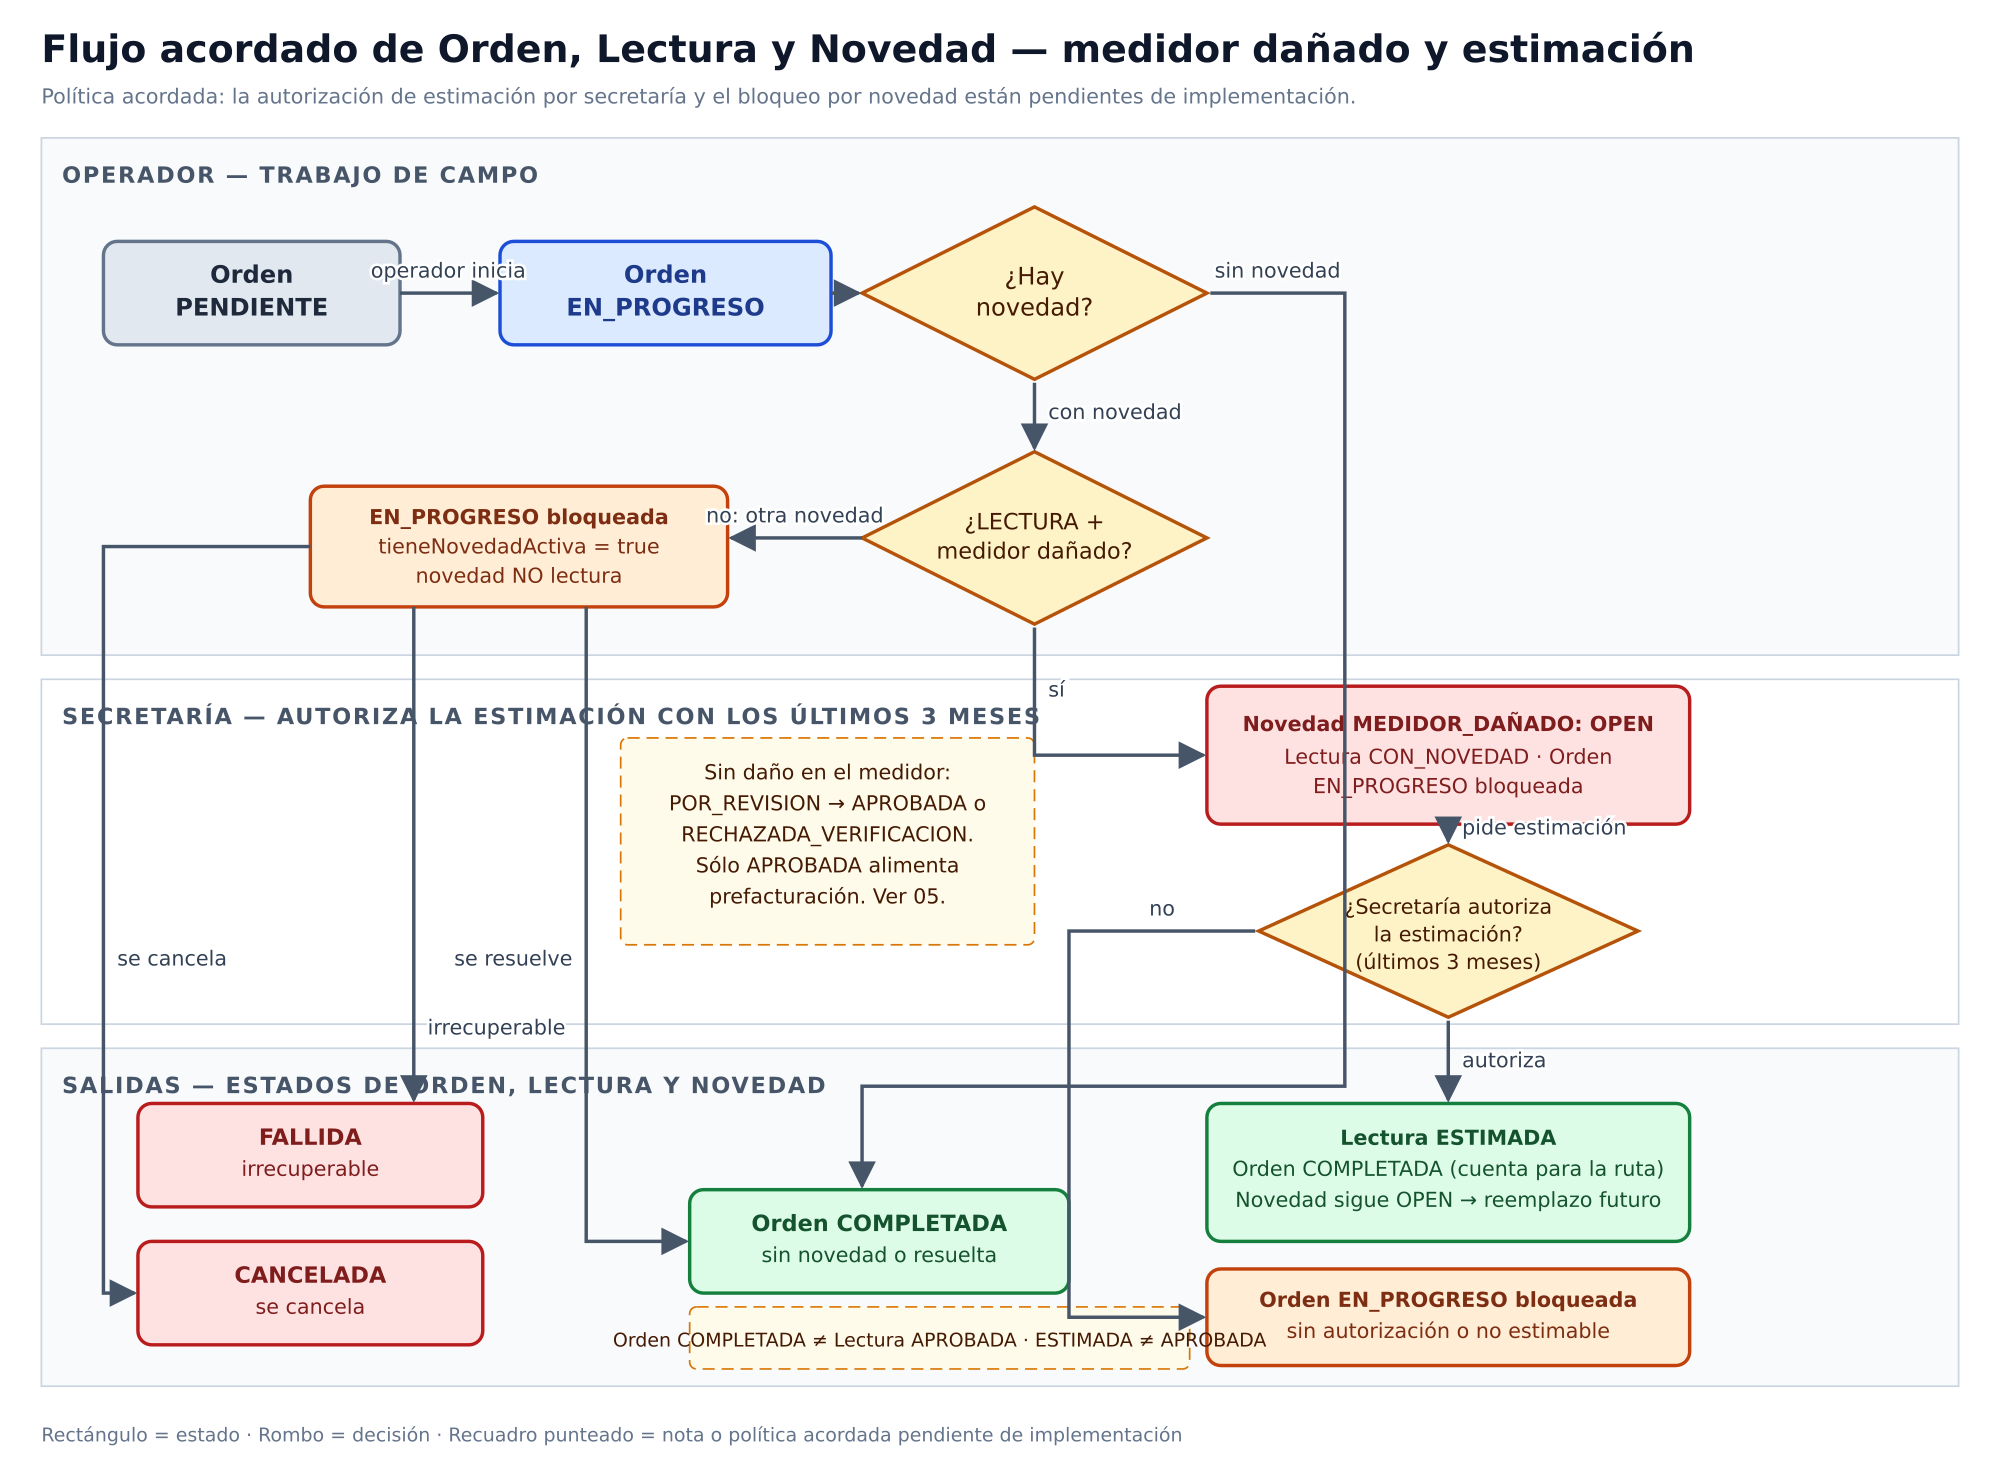
\includegraphics[width=0.95\textwidth]{images/04-orden-lectura-flujo.png}}{\fbox{\parbox{0.88\textwidth}{\centering Flujo acordado: PENDIENTE $\rightarrow$ EN\_PROGRESO $\rightarrow$ COMPLETADA; bloqueo por novedad con {\ttfamily tieneNovedadActiva}; salidas FALLIDA/CANCELADA; estimación autorizada por secretaría.\\[3pt]Agregar \texttt{images/04-orden-lectura-flujo.png} para reemplazar este fallback.}}}
\caption{Flujo acordado de orden, lectura y novedad. Fuente editable: {\ttfamily diagrams/orden-lectura-novedad.drawio}.}
\end{figure}

Resumen textual del flujo:
\begin{itemize}
\item La orden inicia en \texttt{PENDIENTE}; el operador la pasa a \texttt{EN\_PROGRESO} al iniciar el trabajo.
\item Sin novedad, la orden se completa (\texttt{COMPLETADA}).
\item Con novedad en una orden que NO es de lectura, la orden queda en \texttt{EN\_PROGRESO} con \texttt{tieneNovedadActiva=true} hasta resolverla; si el caso es irrecuperable pasa a \texttt{FALLIDA}, y si se cancela pasa a \texttt{CANCELADA}.
\item En una orden de \texttt{LECTURA} con medidor dañado, el operador crea una \texttt{NovedadOrdenTrabajo} en \texttt{OPEN}; la lectura queda en \texttt{CON\_NOVEDAD} y la orden permanece en \texttt{EN\_PROGRESO} bloqueada.
\item Sólo secretaría puede autorizar la estimación con los últimos 3 meses (\textbf{política acordada, pendiente de implementación}): si autoriza, la lectura pasa a \texttt{ESTIMADA} y la orden a \texttt{COMPLETADA}, mientras la novedad sigue en \texttt{OPEN} para un reemplazo futuro; si no autoriza o no se puede estimar, la orden sigue bloqueada.
\item La orden \texttt{COMPLETADA} no implica lectura \texttt{APROBADA}: la estimación genera \texttt{ESTIMADA}, no \texttt{APROBADA}.
\item La orden completada por estimación autorizada cuenta como \texttt{COMPLETADA} para el cierre de la ruta.
\end{itemize}

\texttt{NOVEDAD} no es un valor del enum de \texttt{OrdenTrabajo}: es una condición derivada de la relación con \texttt{NovedadOrdenTrabajo} y de la existencia de novedades activas. No debe persistirse ni confundirse con \texttt{OrdenTrabajo.estado}.

\subsubsection{Tres máquinas separadas}

\begin{center}
\small
\begin{longtable}{|p{0.25\textwidth}|p{0.34\textwidth}|p{0.31\textwidth}|}
\hline
\textbf{Entidad} & \textbf{Máquina} & \textbf{Responsabilidad} \\
\hline
\endfirsthead
\hline
\textbf{Entidad} & \textbf{Máquina} & \textbf{Responsabilidad} \\
\hline
\endhead
\texttt{OrdenTrabajo.estado} & Ejecución operativa: \texttt{PENDIENTE}, \texttt{EN\_PROGRESO}, \texttt{COMPLETADA}, \texttt{CANCELADA}, \texttt{FALLIDA}. & Etapa del trabajo de campo y cierre de la orden. \\
\hline
\texttt{NovedadOrdenTrabajo.estado} & Análisis de anomalía: \texttt{OPEN}, \texttt{IN\_PROGRESS}, \texttt{RESOLVED}, \texttt{CANCELLED}. & Atención, resolución o cancelación de la anomalía. \\
\hline
\texttt{Lectura.estado} & Captura y validación: \texttt{PENDIENTE}, \texttt{POR\_REVISION}, \texttt{APROBADA}, \texttt{RECHAZADA\_VERIFICACION}, \texttt{ESTIMADA}, \texttt{PLANILLADA}, \texttt{CON\_NOVEDAD}. & Ciclo de captura, revisión, aprobación, rechazo o tratamiento del dato. \\
\hline
\end{longtable}
\end{center}

Una novedad activa puede generar una alerta sobre la orden, pero no transforma su estado persistido en \texttt{NOVEDAD}; una lectura con \texttt{CON\_NOVEDAD} tampoco reemplaza el estado de la orden ni el estado de la novedad.

\subsubsection{Ejemplo de respuesta derivada}

\begin{lstlisting}
{
  "ordenTrabajoId": "9",
  "estado": "EN_PROGRESO",
  "tieneNovedadActiva": true,
  "novedadesActivas": [
    {
      "novedadOrdenTrabajoId": "31",
      "estado": "OPEN",
      "tipo": "LECTURA_ERRONEA",
      "observacion": "El visor no permite validar el consumo"
    }
  ]
}
\end{lstlisting}

\subsubsection{Regla de backend y pendiente funcional}

La UI no es la única barrera. Como regla de backend propuesta, una operación no debe permitir pasar la orden a \texttt{COMPLETADA} si existe una novedad abierta que afecte el resultado; la validación debe ejecutarse en el caso de uso o repositorio que completa la orden. Esta regla está pendiente de implementación.

También está pendiente definir el campo o criterio que determina si una novedad es bloqueante: podría ser \texttt{afectaOrden}, el tipo de novedad, la resolución registrada o una regla equivalente. Hasta acordarlo, esta sección documenta una decisión funcional propuesta y no un comportamiento vigente.

También están pendientes de implementación la autorización de la estimación sólo por secretaría con los últimos 3 meses y el conteo de órdenes para el cierre \texttt{COMPLETADA}/\texttt{PARCIAL} de la ruta.


\subsection{Efectos y transacciones}


Crear/actualizar/eliminar rutas y órdenes escriben \texttt{\detokenize{Rutas}}, \texttt{\detokenize{OrdenTrabajo}} y, cuando corresponde, \texttt{\detokenize{EjecucionOrdenTrabajo}}. Vincular una lectura completa la orden y fija \texttt{\detokenize{completadoEn}}; cambiarla a pendiente/en progreso lo limpia. El operador puede almacenar evidencia en RustFS y su clave en la orden. Consultas, filtros, mapeadores y generación PDF son transformaciones puras; la subida de evidencia no lo es.


\begin{center}
\small
\begin{longtable}{|p{0.470\textwidth}|p{0.470\textwidth}|}
\hline
\textbf{Tabla Prisma} & \textbf{Uso} \\
\hline
\endfirsthead
\hline
\textbf{Tabla Prisma} & \textbf{Uso} \\
\hline
\endhead
\texttt{\detokenize{Rutas}} & Ruta, asignación, estado y soft delete. \\
\hline
\texttt{\detokenize{OrdenTrabajo}} & Trabajo y vínculo con lectura. \\
\hline
\texttt{\detokenize{EjecucionOrdenTrabajo}} & Resultado de ejecución. \\
\hline
\texttt{\detokenize{Lecturas}} & Lecturas elegibles/vinculadas. \\
\hline
\texttt{\detokenize{Periodos}} & Ciclo contable. \\
\hline
\texttt{\detokenize{NovedadOrdenTrabajo}} & Novedades de campo. \\
\hline
\end{longtable}
\end{center}


\subsection{Flujos acordados y máquinas de estado}

\begin{figure}[h]
\centering
\IfFileExists{images/04-ruta-flujo.png}{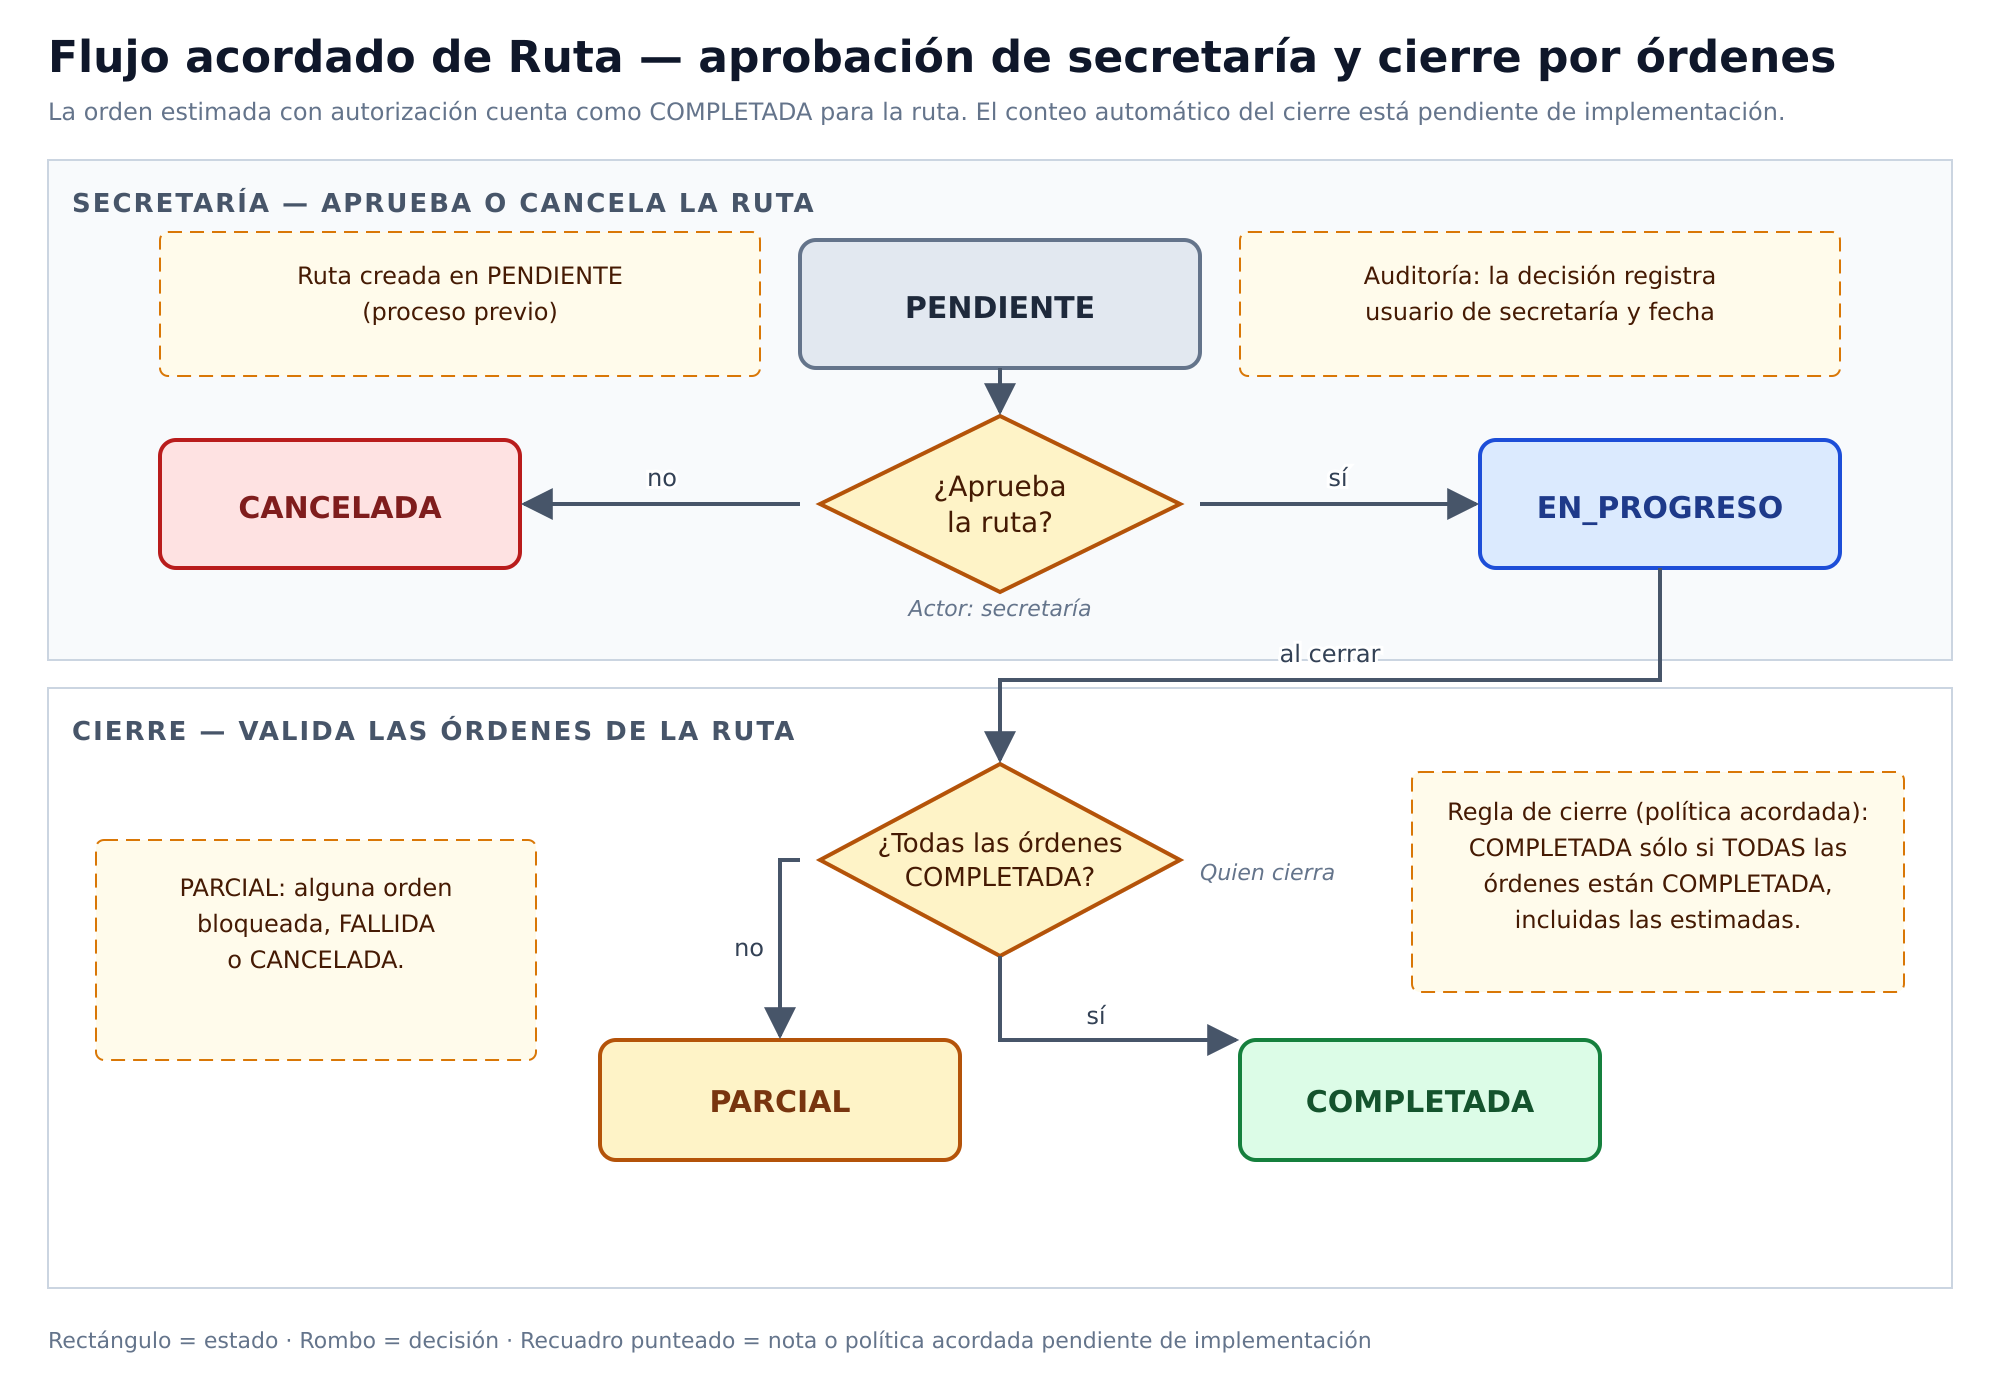
\includegraphics[width=0.95\textwidth]{images/04-ruta-flujo.png}}{\fbox{\parbox{0.88\textwidth}{\centering Flujo acordado de la ruta: PENDIENTE $\rightarrow$ EN\_PROGRESO (aprueba secretaría) o CANCELADA; cierre COMPLETADA/PARCIAL según las órdenes.\\[3pt]Agregar \texttt{images/04-ruta-flujo.png} para reemplazar este fallback.}}}
\caption{Flujo acordado de la ruta. Fuente editable: {\ttfamily diagrams/ruta-estados.drawio}.}
\end{figure}

Resumen textual del flujo:
\begin{itemize}
\item La ruta nace en \texttt{PENDIENTE}.
\item Secretaría decide con auditoría (usuario y fecha): si no la aprueba, la ruta pasa a \texttt{CANCELADA}; si la aprueba, pasa a \texttt{EN\_PROGRESO}.
\item Al cerrar una ruta en \texttt{EN\_PROGRESO} se validan sus órdenes (\textbf{conteo pendiente de implementación}): si TODAS están \texttt{COMPLETADA} —incluidas las completadas por estimación autorizada—, la ruta pasa a \texttt{COMPLETADA}; si alguna sigue bloqueada, o está \texttt{FALLIDA} o \texttt{CANCELADA}, la ruta pasa a \texttt{PARCIAL}.
\end{itemize}

Alcance en código: \texttt{UpdateRouteStateUseCase} confirma las transiciones del operador. \texttt{COMPLETADA} y \texttt{CANCELADA} son terminales en ese caso de uso.

\subsubsection{Estado de la orden}
Alcance: transiciones \textbf{acordadas} (política); los estados del enum y las escrituras están confirmados, pero \texttt{UpdateOrdenEstadoUseCase} no define una tabla de transiciones en código.

\begin{itemize}
\item \texttt{PENDIENTE} $\rightarrow$ \texttt{EN\_PROGRESO}: el operador inicia el trabajo.
\item \texttt{EN\_PROGRESO} $\rightarrow$ \texttt{COMPLETADA}: sin novedad activa, con la novedad resuelta, o con estimación autorizada por secretaría.
\item \texttt{EN\_PROGRESO} $\rightarrow$ \texttt{FALLIDA}: el caso es irrecuperable.
\item \texttt{EN\_PROGRESO} $\rightarrow$ \texttt{CANCELADA}: se cancela el trabajo.
\item Con novedad activa sin resolver, la orden permanece en \texttt{EN\_PROGRESO} con \texttt{tieneNovedadActiva=true} (ver flujo acordado).
\end{itemize}

\subsubsection{Estado de las novedades de órdenes de trabajo}

Sí existe una máquina de estados independiente para \texttt{NovedadOrdenTrabajo}. El modelo Prisma confirma \texttt{OPEN}, \texttt{IN	extunderscore PROGRESS}, \texttt{RESOLVED} y \texttt{CANCELLED}. La novedad se relaciona con una orden y opcionalmente con una lectura y el usuario que la resolvió.

Alcance: \textbf{Confirmado} para los estados, el valor inicial \texttt{OPEN} y los datos de resolución. No se encontró un controlador o caso de uso dedicado que confirme las transiciones HTTP; las flechas de atención y resolución son un flujo esperado.

La máquina, en texto:
\begin{itemize}
\item \texttt{OPEN} (valor inicial al crear la novedad) $\rightarrow$ \texttt{IN\_PROGRESS}: inicia la atención (flujo esperado).
\item \texttt{IN\_PROGRESS} $\rightarrow$ \texttt{RESOLVED}: registra la resolución con usuario y fecha (flujo esperado).
\item \texttt{OPEN} o \texttt{IN\_PROGRESS} $\rightarrow$ \texttt{CANCELLED}: se cancela (flujo esperado, sin reactivación confirmada).
\end{itemize}

La novedad de medidor dañado puede seguir en \texttt{OPEN} después de una estimación autorizada, para gestionar el reemplazo futuro del medidor.

\begin{center}
\small
\begin{longtable}{|p{0.31\textwidth}|p{0.63\textwidth}|}
\hline
\textbf{Elemento} & \textbf{Valores o datos confirmados} \\
\hline
\endfirsthead
\hline
\textbf{Elemento} & \textbf{Valores o datos confirmados} \\
\hline
\endhead
Estado & \texttt{OPEN}, \texttt{IN\textunderscore PROGRESS}, \texttt{RESOLVED}, \texttt{CANCELLED}. \\
\hline
Tipo de anomalía & \texttt{FUGA}, \texttt{MEDIDOR\textunderscore DAÑADO}, \texttt{LECTURA\textunderscore ERRONEA}, \texttt{OTRO}. \\
\hline
Resolución económica & \texttt{COBRO\textunderscore REAL}, \texttt{PROMEDIO\textunderscore HISTORICO}, \texttt{EXONERACION\textunderscore PARCIAL}, \texttt{EXONERACION\textunderscore TOTAL}, \texttt{AJUSTE\textunderscore LECTURA}. \\
\hline
Datos de resolución & \texttt{resolucionTipo}, \texttt{consumoAjustado}, \texttt{observacionResolucion}, \texttt{resueltoPorUsuarioId}, \texttt{resueltoEn}. \\
\hline
\end{longtable}
\end{center}

\texttt{resultadoObservacion} y \texttt{estado=FALLIDA} de \texttt{OrdenesTrabajo} no sustituyen a \texttt{NovedadOrdenTrabajo}: representan el resultado de la orden, mientras que la novedad conserva la anomalía y su resolución.


\subsection{Casos de uso}


\subsubsection{Caso: Consultar períodos}


\textbf{Descripción:} lista períodos disponibles para filtros y asignación.  

\textbf{HTTP y ruta:} \texttt{\detokenize{GET /api/v1/routes/periods}}.  

\textbf{Permiso:} \texttt{\detokenize{routes:read}}.  

\textbf{Cadena:} \texttt{\detokenize{RoutesController.getPeriods()}} → \texttt{\detokenize{RoutesService.getPeriodos()}} → repositorio.  

\textbf{Errores relevantes:} \texttt{\detokenize{401}}; \texttt{\detokenize{403}}.  

\textbf{Efectos:} ninguno.  

\textbf{Prisma:} \texttt{\detokenize{Periodos}}.  

\textbf{Entrada:} sin body ni parámetros.  

\textbf{Salida:}


\begin{lstlisting}
[{"periodoId":12,"nombre":"2026-08","estado":"ACTIVO"}]
\end{lstlisting}


\subsubsection{Caso: Consultar lecturas elegibles}


\textbf{Descripción:} devuelve lecturas disponibles para asignarlas a una ruta.  

\textbf{HTTP y ruta:} \texttt{\detokenize{GET /api/v1/routes/eligible-readings}}.  

\textbf{Permiso:} \texttt{\detokenize{routes:read}}.  

\textbf{Cadena:} \texttt{\detokenize{RoutesController.getEligibleReadings()}} → \texttt{\detokenize{RoutesService.getEligibleReadings()}} → \texttt{\detokenize{GetEligibleReadingsUseCase.execute()}}.  

\textbf{Errores relevantes:} \texttt{\detokenize{400}}; \texttt{\detokenize{401}}; \texttt{\detokenize{403}}.  

\textbf{Efectos:} ninguno.  

\textbf{Prisma:} \texttt{\detokenize{Lecturas}}, \texttt{\detokenize{Contratos}}, \texttt{\detokenize{Medidores}}, \texttt{\detokenize{Periodos}}, \texttt{\detokenize{OrdenTrabajo}}.  

\textbf{Entrada:} sin body; query \texttt{\detokenize{page}}, \texttt{\detokenize{limit}} y filtros de \texttt{\detokenize{FilterReadingsDto}}.  

\textbf{Salida:}


\begin{lstlisting}
{"data":[{"lecturaId":"101","estado":"PENDIENTE"}],"meta":{"page":1,"limit":10,"total":1,"totalPages":1},"kpis":{}}
\end{lstlisting}


\subsubsection{Caso: Consultar lecturas de ruta}


\textbf{Descripción:} lista lecturas ya vinculadas a una ruta.  

\textbf{HTTP y ruta:} \texttt{\detokenize{GET /api/v1/routes/:rutaId/readings}}.  

\textbf{Permiso:} \texttt{\detokenize{routes:read}}.  

\textbf{Cadena:} \texttt{\detokenize{RoutesController.getReadingsByRuta()}} → \texttt{\detokenize{RoutesService.getReadingsByRuta()}} → \texttt{\detokenize{GetReadingsByRutaUseCase.execute()}}.  

\textbf{Errores relevantes:} \texttt{\detokenize{400}}; \texttt{\detokenize{401}}; \texttt{\detokenize{403}}; \texttt{\detokenize{404}}.  

\textbf{Efectos:} ninguno.  

\textbf{Prisma:} \texttt{\detokenize{Rutas}}, \texttt{\detokenize{OrdenTrabajo}}, \texttt{\detokenize{Lecturas}}.  

\textbf{Entrada:} sin body; path \texttt{\detokenize{{ "rutaId": "42" }}}; query \texttt{\detokenize{page}}, \texttt{\detokenize{limit}}.  

\textbf{Salida:}


\begin{lstlisting}
{"data":[{"lecturaId":"101","estado":"PENDIENTE"}],"meta":{"page":1,"limit":10,"total":1,"totalPages":1},"kpis":{}}
\end{lstlisting}


\subsubsection{Caso: Crear ruta}


\textbf{Descripción:} crea una ruta de trabajo con su período y tipo.  

\textbf{HTTP y ruta:} \texttt{\detokenize{POST /api/v1/routes}}.  

\textbf{Permiso:} \texttt{\detokenize{routes:create}}.  

\textbf{Cadena:} \texttt{\detokenize{RoutesController.create()}} → \texttt{\detokenize{RoutesService.create()}} → \texttt{\detokenize{CreateRouteUseCase.execute()}} → repositorio.  

\textbf{Errores relevantes:} \texttt{\detokenize{400}}; \texttt{\detokenize{401}}; \texttt{\detokenize{403}}; \texttt{\detokenize{404}} período/guías.  

\textbf{Efectos:} alta en \texttt{\detokenize{Rutas}} y asociaciones que determine el caso.  

\textbf{Prisma:} \texttt{\detokenize{Rutas}}, \texttt{\detokenize{OrdenTrabajo}}, \texttt{\detokenize{Contratos}}, \texttt{\detokenize{Periodos}}.  

\textbf{Entrada:} body \texttt{\detokenize{{ "nombre": "Lecturas agosto", "tipoRuta": "LECTURA", "periodoId": 12 }}}.  

\textbf{Salida:}


\begin{lstlisting}
{"rutaId":"42","nombre":"Lecturas agosto","estado":"PENDIENTE","ordenesTrabajo":[]}
\end{lstlisting}


\subsubsection{Caso: Listar rutas}


\textbf{Descripción:} devuelve rutas con paginación y filtros.  

\textbf{HTTP y ruta:} \texttt{\detokenize{GET /api/v1/routes}}.  

\textbf{Permiso:} \texttt{\detokenize{routes:read}}.  

\textbf{Cadena:} \texttt{\detokenize{RoutesController.findAll()}} → \texttt{\detokenize{RoutesService.findAll()}} → repositorio.  

\textbf{Errores relevantes:} \texttt{\detokenize{400}}; \texttt{\detokenize{401}}; \texttt{\detokenize{403}}.  

\textbf{Efectos:} ninguno.  

\textbf{Prisma:} \texttt{\detokenize{Rutas}} y relaciones.  

\textbf{Entrada:} sin body; query \texttt{\detokenize{page}}, \texttt{\detokenize{limit}}, \texttt{\detokenize{estado}}, \texttt{\detokenize{operarioId}}, \texttt{\detokenize{comunidadId}}, \texttt{\detokenize{periodoId}}, \texttt{\detokenize{tipoRuta}}.  

\textbf{Salida:}


\begin{lstlisting}
{"data":[{"rutaId":"42","estado":"PENDIENTE"}],"meta":{"page":1,"limit":10,"total":1,"totalPages":1}}
\end{lstlisting}


\subsubsection{Caso: Obtener ruta}


\textbf{Descripción:} consulta una ruta por ID.  

\textbf{HTTP y ruta:} \texttt{\detokenize{GET /api/v1/routes/:id}}.  

\textbf{Permiso:} \texttt{\detokenize{routes:read}}.  

\textbf{Cadena:} \texttt{\detokenize{RoutesController.findOne()}} → \texttt{\detokenize{RoutesService.findOne()}} → repositorio.  

\textbf{Errores relevantes:} \texttt{\detokenize{400}}; \texttt{\detokenize{401}}; \texttt{\detokenize{403}}; \texttt{\detokenize{404}}.  

\textbf{Efectos:} ninguno.  

\textbf{Prisma:} \texttt{\detokenize{Rutas}}, \texttt{\detokenize{OrdenTrabajo}}, \texttt{\detokenize{Contratos}}, \texttt{\detokenize{Periodos}}.  

\textbf{Entrada:} sin body; path \texttt{\detokenize{{ "id": "42" }}}.  

\textbf{Salida:}


\begin{lstlisting}
{"rutaId":"42","estado":"PENDIENTE","ordenesTrabajo":[]}
\end{lstlisting}


\subsubsection{Caso: Actualizar ruta}


\textbf{Descripción:} modifica los datos de una ruta existente.  

\textbf{HTTP y ruta:} \texttt{\detokenize{PATCH /api/v1/routes/:id}}.  

\textbf{Permiso:} \texttt{\detokenize{routes:update}}.  

\textbf{Cadena:} \texttt{\detokenize{RoutesController.update()}} → \texttt{\detokenize{RoutesService.update()}} → \texttt{\detokenize{UpdateRouteUseCase.execute()}} → repositorio.  

\textbf{Errores relevantes:} \texttt{\detokenize{400}}; \texttt{\detokenize{401}}; \texttt{\detokenize{403}}; \texttt{\detokenize{404}}.  

\textbf{Efectos:} actualización de \texttt{\detokenize{Rutas}}; DTO puro.  

\textbf{Prisma:} \texttt{\detokenize{Rutas}}.  

\textbf{Entrada:} path \texttt{\detokenize{{ "id": "42" }}}; body \texttt{\detokenize{{ "nombre": "Ruta actualizada" }}}.  

\textbf{Salida:} \texttt{\detokenize{{ "rutaId": "42", "nombre": "Ruta actualizada", "estado": "PENDIENTE" }}}.


\subsubsection{Caso: Reasignar ruta}


\textbf{Descripción:} asigna o desasigna la ruta a un operario.  

\textbf{HTTP y ruta:} \texttt{\detokenize{PATCH /api/v1/routes/:id/reassign}}.  

\textbf{Permiso:} \texttt{\detokenize{routes:update}}.  

\textbf{Cadena:} \texttt{\detokenize{RoutesController.reassign()}} → \texttt{\detokenize{ReassignRouteUseCase.execute()}} → repositorio.  

\textbf{Errores relevantes:} \texttt{\detokenize{400}}; \texttt{\detokenize{401}}; \texttt{\detokenize{403}}; \texttt{\detokenize{404}}; ruta ya asignada.  

\textbf{Efectos:} cambia \texttt{\detokenize{Rutas.operarioId}}.  

\textbf{Prisma:} \texttt{\detokenize{Rutas}}, \texttt{\detokenize{Usuarios/Operarios}}.  

\textbf{Entrada:} path \texttt{\detokenize{{ "id": "42" }}}; body \texttt{\detokenize{{ "operarioId": "7" }}} o \texttt{\detokenize{null}}.  

\textbf{Salida:} \texttt{\detokenize{{ "rutaId": "42", "operarioId": 7, "estado": "PENDIENTE" }}}.


\subsubsection{Caso: Eliminar ruta}


\textbf{Descripción:} elimina lógicamente la ruta.  

\textbf{HTTP y ruta:} \texttt{\detokenize{DELETE /api/v1/routes/:id}}.  

\textbf{Permiso:} \texttt{\detokenize{routes:delete}}.  

\textbf{Cadena:} \texttt{\detokenize{RoutesController.delete()}} → \texttt{\detokenize{RoutesService.delete()}} → \texttt{\detokenize{DeleteRouteUseCase.execute()}} → repositorio.  

\textbf{Errores relevantes:} \texttt{\detokenize{400}}; \texttt{\detokenize{401}}; \texttt{\detokenize{403}}; \texttt{\detokenize{404}}.  

\textbf{Efectos:} soft delete y desasignación según el caso.  

\textbf{Prisma:} \texttt{\detokenize{Rutas}}, \texttt{\detokenize{OrdenTrabajo}}, \texttt{\detokenize{Lecturas}}.  

\textbf{Entrada:} sin body; path \texttt{\detokenize{{ "id": "42" }}}.  

\textbf{Salida:} \texttt{\detokenize{{ "rutaId": "42", "estado": "CANCELADA" }}}.


\subsubsection{Caso: Exportar hoja de campo}


\textbf{Descripción:} genera la hoja oficial de órdenes y lecturas.  

\textbf{HTTP y ruta:} \texttt{\detokenize{GET /api/v1/routes/:id/pdf}}.  

\textbf{Permiso:} \texttt{\detokenize{routes:read}}.  

\textbf{Cadena:} \texttt{\detokenize{RoutesController.exportPdf()}} → \texttt{\detokenize{RoutesService.exportPdf()}} → \texttt{\detokenize{ExportFieldSheetPdfUseCase}}/generador.  

\textbf{Errores relevantes:} \texttt{\detokenize{400}}; \texttt{\detokenize{401}}; \texttt{\detokenize{403}}; \texttt{\detokenize{404}}.  

\textbf{Efectos:} lectura y generación puras.  

\textbf{Prisma:} \texttt{\detokenize{Rutas}}, \texttt{\detokenize{OrdenTrabajo}}, \texttt{\detokenize{Lecturas}}.  

\textbf{Entrada:} sin body; path \texttt{\detokenize{{ "id": "42" }}}.  

\textbf{Salida:} no es JSON: \texttt{\detokenize{application/pdf}}, \texttt{\detokenize{Content-Disposition: inline}}, \texttt{\detokenize{Content-Length}} y bytes PDF.


\subsubsection{Caso: Consultar órdenes de una ruta}


\textbf{Descripción:} lista órdenes asociadas, filtradas y paginadas.  

\textbf{HTTP y ruta:} \texttt{\detokenize{GET /api/v1/routes/:id/work-orders}}.  

\textbf{Permiso:} \texttt{\detokenize{routes:read}}.  

\textbf{Cadena:} \texttt{\detokenize{RoutesController.findOrdenesByRuta()}} → \texttt{\detokenize{OrdenesTrabajoService.findByRuta()}} → \texttt{\detokenize{FindOrdenesByRutaUseCase.execute()}}.  

\textbf{Errores relevantes:} \texttt{\detokenize{400}}; \texttt{\detokenize{401}}; \texttt{\detokenize{403}}; \texttt{\detokenize{404}}.  

\textbf{Efectos:} ninguno.  

\textbf{Prisma:} \texttt{\detokenize{OrdenTrabajo}}, \texttt{\detokenize{Rutas}}, \texttt{\detokenize{Lecturas}}.  

\textbf{Entrada:} sin body; path \texttt{\detokenize{{ "id": "42" }}}; query \texttt{\detokenize{estado}}, \texttt{\detokenize{page}}, \texttt{\detokenize{limit}}.  

\textbf{Salida:} \texttt{\detokenize{{ "data": [{ "ordenTrabajoId": "9", "estado": "PENDIENTE" }], "meta": {}, "kpis": {} }}}.


\subsubsection{Caso: Actualizar estado de orden}


\textbf{Descripción:} cambia estado, observación y fecha de finalización de una orden.  

\textbf{HTTP y ruta:} \texttt{\detokenize{PATCH /api/v1/work-orders/:id/state}}.  

\textbf{Permiso:} \texttt{\detokenize{routes:update}}.  

\textbf{Cadena:} \texttt{\detokenize{OrdenesTrabajoController.updateEstado()}} → \texttt{\detokenize{OrdenesTrabajoService.updateEstado()}} → \texttt{\detokenize{UpdateOrdenEstadoUseCase.execute()}} → repositorio.  

\textbf{Errores relevantes:} \texttt{\detokenize{400}}; \texttt{\detokenize{401}}; \texttt{\detokenize{403}}; \texttt{\detokenize{404}}; \texttt{\detokenize{409}}.  

\textbf{Efectos:} persiste estado; completa o limpia \texttt{\detokenize{completadoEn}}.  

\textbf{Prisma:} \texttt{\detokenize{OrdenTrabajo}}, \texttt{\detokenize{EjecucionOrdenTrabajo}}.  

\textbf{Entrada:} path \texttt{\detokenize{{ "id": "9" }}}; body \texttt{\detokenize{{ "estado": "COMPLETADA", "resultadoObservacion": "Trabajo realizado" }}}.  

\textbf{Salida:} \texttt{\detokenize{{ "ordenTrabajoId": "9", "estado": "COMPLETADA" }}}.


\subsubsection{Caso: Vincular lectura a orden}


\textbf{Descripción:} asocia una lectura y completa la orden.  

\textbf{HTTP y ruta:} \texttt{\detokenize{PATCH /api/v1/work-orders/:id/reading}}.  

\textbf{Permiso:} \texttt{\detokenize{routes:update}}.  

\textbf{Cadena:} \texttt{\detokenize{OrdenesTrabajoController.linkLectura()}} → \texttt{\detokenize{OrdenesTrabajoService.linkLectura()}} → \texttt{\detokenize{LinkLecturaUseCase.execute()}} → repositorio.  

\textbf{Errores relevantes:} \texttt{\detokenize{400}}; \texttt{\detokenize{401}}; \texttt{\detokenize{403}}; \texttt{\detokenize{404}}; \texttt{\detokenize{409}}.  

\textbf{Efectos:} persiste vínculo y \texttt{\detokenize{completadoEn}}.  

\textbf{Prisma:} \texttt{\detokenize{OrdenTrabajo}}, \texttt{\detokenize{Lecturas}}, \texttt{\detokenize{Rutas}}.  

\textbf{Entrada:} path \texttt{\detokenize{{ "id": "9" }}}; body \texttt{\detokenize{{ "lecturaId": "101" }}}.  

\textbf{Salida:} \texttt{\detokenize{{ "ordenTrabajoId": "9", "lecturaId": "101", "estado": "COMPLETADA" }}}.


\subsubsection{Caso: Actualizar operación del operador}


\textbf{Descripción:} registra ejecución y evidencia opcional de una orden.  

\textbf{HTTP y ruta:} \texttt{\detokenize{PATCH /api/v1/operator/work-orders/:id}}.  

\textbf{Permiso:} \texttt{\detokenize{routes:update}}.  

\textbf{Cadena:} \texttt{\detokenize{OperatorController.updateOperatorWorkOrder()}} → \texttt{\detokenize{UpdateOperatorWorkOrderUseCase.execute()}} → repositorio/RustFS.  

\textbf{Errores relevantes:} \texttt{\detokenize{400}}; \texttt{\detokenize{401}}; \texttt{\detokenize{403}}; \texttt{\detokenize{404}}; \texttt{\detokenize{409}}.  

\textbf{Efectos:} persiste ejecución y \texttt{\detokenize{evidenciaFotoUrl}}; la subida y rollback de archivo son efectos reales.  

\textbf{Prisma:} \texttt{\detokenize{OrdenTrabajo}}, \texttt{\detokenize{EjecucionOrdenTrabajo}}, \texttt{\detokenize{NovedadOrdenTrabajo}}.  

\textbf{Entrada:} path \texttt{\detokenize{{ "id": "9" }}}; multipart: campos DTO y archivo opcional \texttt{\detokenize{foto}}; sin body JSON.  

\textbf{Salida:} JSON \texttt{\detokenize{OrderWorkResponseDto}}, por ejemplo \texttt{\detokenize{{ "ordenTrabajoId": "9", "estado": "COMPLETADA", "evidenciaFotoUrl": "ordenes/9/foto.jpg" }}}.


\subsubsection{Caso: Listar rutas del operador}


\textbf{Descripción:} lista las rutas del período activo asignadas al operador autenticado.  

\textbf{HTTP y ruta:} \texttt{\detokenize{GET /api/v1/operator/routes}}.  

\textbf{Permiso:} \texttt{\detokenize{routes:read}}.  

\textbf{Cadena:} \texttt{\detokenize{OperatorController.getOperatorRoutes()}} → \texttt{\detokenize{GetOperatorRoutesUseCase.execute()}} → repositorio.  

\textbf{Errores relevantes:} \texttt{\detokenize{400}}; \texttt{\detokenize{401}}; \texttt{\detokenize{403}}; \texttt{\detokenize{404}} sin período activo.  

\textbf{Efectos:} ninguno; consulta y DTO puros.  

\textbf{Prisma:} \texttt{\detokenize{Rutas}}, \texttt{\detokenize{OrdenTrabajo}}, \texttt{\detokenize{Periodos}}.  

\textbf{Entrada:} sin body; query opcional \texttt{\detokenize{tipoRuta}}; operador desde JWT.  

\textbf{Salida:} lista JSON de \texttt{\detokenize{OperatorRouteResponseDto}}.


\subsubsection{Caso: Actualizar estado de ruta del operador}


\textbf{Descripción:} cambia el estado de una ruta que pertenece al operador autenticado.  

\textbf{HTTP y ruta:} \texttt{\detokenize{PATCH /api/v1/operator/routes/:id/state}}.  

\textbf{Permiso:} \texttt{\detokenize{routes:update}}.  

\textbf{Cadena:} \texttt{\detokenize{OperatorController.updateRouteState()}} → \texttt{\detokenize{UpdateRouteStateUseCase.execute()}} → repositorio.  

\textbf{Errores relevantes:} \texttt{\detokenize{400}}; \texttt{\detokenize{401}}; \texttt{\detokenize{403}} ruta ajena; \texttt{\detokenize{404}}; \texttt{\detokenize{409}} transición inválida.  

\textbf{Efectos:} actualiza \texttt{\detokenize{Rutas}} y las marcas temporales derivadas del estado.  

\textbf{Prisma:} \texttt{\detokenize{Rutas}}, \texttt{\detokenize{OrdenTrabajo}}, \texttt{\detokenize{Periodos}}.  

\textbf{Entrada:} path \texttt{\detokenize{{ "id": "42" }}}; body \texttt{\detokenize{{ "estado": "EN_PROGRESO" }}}.  

\textbf{Salida:} \texttt{\detokenize{{ "rutaId": "42", "estado": "EN_PROGRESO" }}}.


\subsection{Pendientes funcionales}

Bloqueos confirmados como pendientes en el código revisado. Cuando se cierre cada uno, sacar de acá y mover a la sección correspondiente.

\begin{itemize}
\item \textbf{Bloqueo por novedad activa al transicionar la orden a \texttt{COMPLETADA}.} El helper \texttt{applyContractLifecycleTransition} solo valida estado origen del contrato, no valida \texttt{tieneNovedadActiva}. Falta decidir el criterio bloqueante (\texttt{afectaOrden}, tipo de novedad o resolución) e implementar la validación en \texttt{UpdateOrdenEstadoUseCase} o en el repositorio de órdenes.
\item \textbf{Autorización exclusiva del rol \texttt{Secretaría} para la estimación con los últimos 3 meses.} Mismo punto pendiente en \texttt{05-lecturas.md}. Requiere endpoint nuevo o permiso específico (\texttt{estimates:approve} o equivalente). La política está acordada pero no está aplicada en código.
\item \textbf{Conteo automático de órdenes para el cierre de la ruta} (\texttt{COMPLETADA} vs \texttt{PARCIAL}). Si TODAS las órdenes están \texttt{COMPLETADA} (incluidas completadas por estimación), la ruta pasa a \texttt{COMPLETADA}; si alguna está \texttt{FALLIDA} o \texttt{CANCELADA}, pasa a \texttt{PARCIAL}. Hoy \texttt{UpdateRouteUseCase} no implementa esa lógica; el estado final lo asigna manualmente quien cierre la ruta.
\item \textbf{Endpoints HTTP para gestión manual de \texttt{NovedadOrdenTrabajo}.} Hoy la entidad solo tiene repositorio; la creación y actualización de novedades ocurre internamente desde otros flujos (captura de lecturas, reporte de defectos). Si el operador debe poder crear/actualizar/resolver novedades desde la UI, falta el controller + use cases correspondientes.
\item \textbf{Auditoría de la decisión de secretaría al aprobar una ruta para \texttt{EN\_PROGRESO}} (usuario y fecha). El documento lo menciona en la sección de flujo acordado de la ruta pero no indica tabla ni columnas donde se persiste esa decisión.
\item \textbf{Tipo de novedad \texttt{INSPECCION} sin efecto sobre ciclo de vida del contrato.} El helper \texttt{applyContractLifecycleTransition} solo reconoce los tipos \texttt{INSTALACION} y \texttt{RECONEXION}. Si una orden de inspección tiene contrato asociado, el efecto sobre el estado del contrato queda indefinido.
\end{itemize}

\subsection{No documentado o pendiente de confirmar}


\begin{itemize}
\item Lista exhaustiva de transiciones de operador.
\item Endpoints legacy basados en \texttt{\detokenize{EstadoAsignacion}}.
\end{itemize}

\section{Lecturas}


Captura, revisión y operación de lecturas de consumo.


\begin{quote}
\textbf{Ficha de dominio:} documenta consulta, revisión administrativa y captura de lecturas por operador, con sus anomalías, evidencias y estados confirmados.
\end{quote}


\subsection{Alcance y entradas HTTP}


\begin{itemize}
\item \textbf{Controladores:} \texttt{\detokenize{ReadingController}}, \texttt{\detokenize{OperatorController}}.
\item \textbf{Servicio:} \texttt{\detokenize{ReadingService}}.
\item \textbf{Casos:} \texttt{\detokenize{FindAllReadingsUseCase}}, \texttt{\detokenize{FindOneReadingUseCase}}, \texttt{\detokenize{UpdateReadingUseCase}}, \texttt{\detokenize{RemoveReadingUseCase}}, \texttt{\detokenize{GetOperatorReadingsUseCase}}, \texttt{\detokenize{GetOperatorReadingsWithAnomaliesUseCase}}, \texttt{\detokenize{UpdateOperatorReadingUseCase}}.
\item El catálogo \texttt{\detokenize{GET /estados}} se construye desde el enum y no tiene servicio/caso dedicado.
\end{itemize}

\subsection{Comportamiento de negocio verificable}
Las tablas relacionadas son \texttt{Lecturas}, \texttt{Contratos}, \texttt{Medidores}, \texttt{Periodos}, \texttt{Rutas}, \texttt{OrdenTrabajo} y \texttt{NovedadOrdenTrabajo}. El flujo confirmado es captura $\rightarrow$ revisión $\rightarrow$ aprobación/rechazo. No se encontró handler de pagos ni promoción automática a planilla.


\begin{center}
\small
\begin{longtable}{|p{0.313\textwidth}|p{0.313\textwidth}|p{0.313\textwidth}|}
\hline
\textbf{Método y ruta} & \textbf{Caso/servicio ejecutado} & \textbf{Resultado} \\
\hline
\endfirsthead
\hline
\textbf{Método y ruta} & \textbf{Caso/servicio ejecutado} & \textbf{Resultado} \\
\hline
\endhead
\texttt{\detokenize{GET /api/v1/readings}} & \texttt{\detokenize{findAll()}} → \texttt{\detokenize{FindAllReadingsUseCase}} & Página. \\
\hline
\texttt{\detokenize{GET /api/v1/readings/estados}} & \texttt{\detokenize{getEstados()}} → \texttt{\detokenize{buildStateCatalog()}} & Catálogo. \\
\hline
\texttt{\detokenize{GET /api/v1/readings/:id}} & \texttt{\detokenize{findOne()}} → \texttt{\detokenize{FindOneReadingUseCase}} & Lectura. \\
\hline
\texttt{\detokenize{PATCH /api/v1/readings/:id}} & \texttt{\detokenize{update()}} → \texttt{\detokenize{UpdateReadingUseCase}} & Lectura actualizada. \\
\hline
\texttt{\detokenize{DELETE /api/v1/readings/:id}} & \texttt{\detokenize{delete()}} → \texttt{\detokenize{RemoveReadingUseCase}}/repositorio & Soft delete. \\
\hline
\texttt{\detokenize{GET /api/v1/operator/readings}} & \texttt{\detokenize{GetOperatorReadingsUseCase}} & Lecturas propias. \\
\hline
\texttt{\detokenize{GET /api/v1/operator/readings/anomalies}} & \texttt{\detokenize{GetOperatorReadingsWithAnomaliesUseCase}} & Anomalías pendientes. \\
\hline
\texttt{\detokenize{PATCH /api/v1/operator/readings/:id}} & \texttt{\detokenize{UpdateOperatorReadingUseCase}} & Lectura/evidencia. \\
\hline
\end{longtable}
\end{center}


\subsection{Ejemplo JSON}


\begin{lstlisting}
{
  "lecturaId": "101",
  "fecha": "2026-08-19",
  "lecturaAnterior": 500,
  "lecturaActual": 530,
  "consumoCalculado": 30,
  "estado": "APROBADA"
}
\end{lstlisting}


\begin{center}
\small
\begin{longtable}{|p{0.313\textwidth}|p{0.313\textwidth}|p{0.313\textwidth}|}
\hline
\textbf{Campo} & \textbf{Tipo} & \textbf{Regla/uso} \\
\hline
\endfirsthead
\hline
\textbf{Campo} & \textbf{Tipo} & \textbf{Regla/uso} \\
\hline
\endhead
\texttt{\detokenize{lecturaId}} & string & \texttt{\detokenize{BigInt}} serializado. \\
\hline
\texttt{\detokenize{fecha}} & string & Fecha de lectura. \\
\hline
\texttt{\detokenize{lecturaAnterior}}, \texttt{\detokenize{lecturaActual}}, \texttt{\detokenize{consumoCalculado}} & number & Valores y diferencia de consumo. \\
\hline
\texttt{\detokenize{estado}} & enum & Revisión y resultado. \\
\hline
\texttt{\detokenize{evidenciaFotoUrl}} & string/null & Evidencia de la orden vinculada cuando aplica. \\
\hline
\end{longtable}
\end{center}


\subsection{Estados}


\begin{center}
\small
\begin{longtable}{|p{0.470\textwidth}|p{0.470\textwidth}|}
\hline
\textbf{Estado} & \textbf{Significado} \\
\hline
\endfirsthead
\hline
\textbf{Estado} & \textbf{Significado} \\
\hline
\endhead
\texttt{\detokenize{PENDIENTE}} & Capturada y aún no revisada. \\
\hline
\texttt{\detokenize{POR_REVISION}} & Requiere validación. \\
\hline
\texttt{\detokenize{APROBADA}} & Elegible para prefacturación. \\
\hline
\texttt{\detokenize{RECHAZADA_VERIFICACION}} & Rechazada. \\
\hline
\texttt{\detokenize{ESTIMADA}} & Valor estimado. \\
\hline
\texttt{\detokenize{PLANILLADA}} & Incorporada a planilla. \\
\hline
\texttt{\detokenize{CON_NOVEDAD}} & Tiene anomalía/novedad. \\
\hline
\end{longtable}
\end{center}


\subsection{Efectos y transacciones}


La actualización administrativa persiste \texttt{\detokenize{Lecturas}} y protege el cambio con control de concurrencia. La operación del operador puede persistir lectura, novedad y evidencia en RustFS; si falla, elimina la foto recién subida. Consultas, resta de consumo y DTO son transformaciones puras. DELETE usa soft delete.


\begin{center}
\small
\begin{longtable}{|p{0.470\textwidth}|p{0.470\textwidth}|}
\hline
\textbf{Tabla Prisma} & \textbf{Uso} \\
\hline
\endfirsthead
\hline
\textbf{Tabla Prisma} & \textbf{Uso} \\
\hline
\endhead
\texttt{\detokenize{Lecturas}} & Valores, estado y soft delete. \\
\hline
\texttt{\detokenize{Contratos}}, \texttt{\detokenize{Medidores}}, \texttt{\detokenize{Periodos}} & Contexto de lectura. \\
\hline
\texttt{\detokenize{OrdenTrabajo}}, \texttt{\detokenize{NovedadOrdenTrabajo}} & Operación y anomalías. \\
\hline
\end{longtable}
\end{center}


\subsection{Gráfico de estados}


\begin{lstlisting}
stateDiagram-v2
  PENDIENTE --> POR_REVISION
  POR_REVISION --> APROBADA
  POR_REVISION --> RECHAZADA_VERIFICACION
\end{lstlisting}


\subsection{Casos de uso}


\subsubsection{Caso: Listar lecturas}


\textbf{Descripción:} devuelve lecturas filtradas y paginadas.  

\textbf{HTTP y ruta:} \texttt{\detokenize{GET /api/v1/readings}}.  

\textbf{Permiso:} \texttt{\detokenize{lecturas:read}}.  

\textbf{Cadena:} \texttt{\detokenize{ReadingController.findAll()}} → \texttt{\detokenize{ReadingService.findAll()}} → \texttt{\detokenize{FindAllReadingsUseCase.execute()}} → repositorio.  

\textbf{Errores relevantes:} \texttt{\detokenize{400}}; \texttt{\detokenize{401}}; \texttt{\detokenize{403}}.  

\textbf{Efectos:} ninguno; lectura y DTO puros.  

\textbf{Prisma:} \texttt{\detokenize{Lecturas}}, \texttt{\detokenize{Contratos}}, \texttt{\detokenize{Medidores}}, \texttt{\detokenize{Periodos}}.  

\textbf{Entrada:} sin body; query \texttt{\detokenize{page}}, \texttt{\detokenize{limit}}, \texttt{\detokenize{contratoId}}, \texttt{\detokenize{estado}}, \texttt{\detokenize{search}}.  

\textbf{Salida:} \texttt{\detokenize{{ "data": [{ "lecturaId": "101", "estado": "PENDIENTE" }], "meta": {} }}}.


\subsubsection{Caso: Consultar catálogo de estados}


\textbf{Descripción:} entrega etiquetas e iconos de \texttt{\detokenize{EstadoLectura}}.  

\textbf{HTTP y ruta:} \texttt{\detokenize{GET /api/v1/readings/estados}}.  

\textbf{Permiso:} \texttt{\detokenize{lecturas:read}}.  

\textbf{Cadena:} \texttt{\detokenize{ReadingController.getEstados()}} → \texttt{\detokenize{buildStateCatalog()}} (sin caso dedicado).  

\textbf{Errores relevantes:} \texttt{\detokenize{401}}; \texttt{\detokenize{403}}.  

\textbf{Efectos:} ninguno.  

\textbf{Prisma:} ninguna tabla.  

\textbf{Entrada:} sin body, path ni query.  

\textbf{Salida:} \texttt{\detokenize{[{ "codigo": "APROBADA", "descripcion": "Aprobada", "icono": "bi-check-circle" }]}}.


\subsubsection{Caso: Obtener lectura}


\textbf{Descripción:} devuelve una lectura por ID.  

\textbf{HTTP y ruta:} \texttt{\detokenize{GET /api/v1/readings/:id}}.  

\textbf{Permiso:} \texttt{\detokenize{lecturas:read}}.  

\textbf{Cadena:} \texttt{\detokenize{ReadingController.findOne()}} → \texttt{\detokenize{ReadingService.findOne()}} → \texttt{\detokenize{FindOneReadingUseCase.execute()}} → repositorio.  

\textbf{Errores relevantes:} \texttt{\detokenize{400}}; \texttt{\detokenize{401}}; \texttt{\detokenize{403}}; \texttt{\detokenize{404}}.  

\textbf{Efectos:} ninguno; DTO puro.  

\textbf{Prisma:} \texttt{\detokenize{Lecturas}}, \texttt{\detokenize{Medidores}}, \texttt{\detokenize{Periodos}}, \texttt{\detokenize{Contratos}}.  

\textbf{Entrada:} sin body; path \texttt{\detokenize{{ "id": "101" }}}.  

\textbf{Salida:} el JSON del ejemplo principal.


\subsubsection{Caso: Actualizar lectura administrativa}


\textbf{Descripción:} actualiza campos no fotográficos y estado.  

\textbf{HTTP y ruta:} \texttt{\detokenize{PATCH /api/v1/readings/:id}}.  

\textbf{Permiso:} \texttt{\detokenize{lecturas:update}}.  

\textbf{Cadena:} \texttt{\detokenize{ReadingController.actualizarLectura()}} → \texttt{\detokenize{ReadingService.update()}} → \texttt{\detokenize{UpdateReadingUseCase.execute()}} → repositorio.  

\textbf{Errores relevantes:} \texttt{\detokenize{400}} body/transición/CAS; \texttt{\detokenize{401}}; \texttt{\detokenize{403}}; \texttt{\detokenize{404}}; \texttt{\detokenize{409}}.  

\textbf{Efectos:} persiste lectura; cálculo y DTO puros.  

\textbf{Prisma:} \texttt{\detokenize{Lecturas}}, \texttt{\detokenize{Medidores}}, \texttt{\detokenize{OrdenTrabajo}}, \texttt{\detokenize{NovedadOrdenTrabajo}}.  

\textbf{Entrada:} path \texttt{\detokenize{{ "id": "101" }}}; body \texttt{\detokenize{{ "lecturaActual": 530, "estado": "POR_REVISION" }}}.  

\textbf{Salida:} \texttt{\detokenize{{ "lecturaId": "101", "lecturaActual": 530, "consumoCalculado": 30, "estado": "POR_REVISION" }}}.


\subsubsection{Caso: Eliminar lectura}


\textbf{Descripción:} aplica eliminación lógica.  

\textbf{HTTP y ruta:} \texttt{\detokenize{DELETE /api/v1/readings/:id}}.  

\textbf{Permiso:} \texttt{\detokenize{lecturas:delete}}.  

\textbf{Cadena:} \texttt{\detokenize{ReadingController.eliminarLectura()}} → \texttt{\detokenize{ReadingService.delete()}} → \texttt{\detokenize{RemoveReadingUseCase}}/repositorio.  

\textbf{Errores relevantes:} \texttt{\detokenize{400}}; \texttt{\detokenize{401}}; \texttt{\detokenize{403}}; \texttt{\detokenize{404}}.  

\textbf{Efectos:} establece \texttt{\detokenize{deletedAt}} en \texttt{\detokenize{Lecturas}}.  

\textbf{Prisma:} \texttt{\detokenize{Lecturas}}.  

\textbf{Entrada:} sin body; path \texttt{\detokenize{{ "id": "101" }}}.  

\textbf{Salida:} \texttt{\detokenize{{ "message": "Lectura eliminada" }}}.


\subsubsection{Caso: Listar lecturas del operador}


\textbf{Descripción:} devuelve las lecturas del período activo asignadas al operador autenticado.  

\textbf{HTTP y ruta:} \texttt{\detokenize{GET /api/v1/operator/readings}}.  

\textbf{Permiso:} \texttt{\detokenize{lecturas:read}}.  

\textbf{Cadena:} \texttt{\detokenize{OperatorController.getOperatorReadings()}} → \texttt{\detokenize{GetOperatorReadingsUseCase.execute()}} → repositorio y DTO.  

\textbf{Errores relevantes:} \texttt{\detokenize{400}}; \texttt{\detokenize{401}}; \texttt{\detokenize{403}}; \texttt{\detokenize{404}} sin período activo.  

\textbf{Efectos:} ninguno; consulta y DTO puros.  

\textbf{Prisma:} \texttt{\detokenize{Lecturas}}, \texttt{\detokenize{Rutas}}, \texttt{\detokenize{OrdenTrabajo}}, \texttt{\detokenize{Periodos}}.  

\textbf{Entrada:} sin body ni query; operador desde JWT.  

\textbf{Salida:} lista JSON de \texttt{\detokenize{ResponseReadingDto}}.


\subsubsection{Caso: Listar anomalías pendientes del operador}


\textbf{Descripción:} devuelve las lecturas del operador que tienen anomalías pendientes de atención.  

\textbf{HTTP y ruta:} \texttt{\detokenize{GET /api/v1/operator/readings/anomalies}}.  

\textbf{Permiso:} \texttt{\detokenize{lecturas:read}}.  

\textbf{Cadena:} \texttt{\detokenize{OperatorController.getOperatorReadingsWithAnomalies()}} → \texttt{\detokenize{GetOperatorReadingsWithAnomaliesUseCase.execute()}} → repositorios y DTO.  

\textbf{Errores relevantes:} \texttt{\detokenize{400}}; \texttt{\detokenize{401}}; \texttt{\detokenize{403}}; \texttt{\detokenize{404}} sin período activo.  

\textbf{Efectos:} ninguno; consulta y DTO puros.  

\textbf{Prisma:} \texttt{\detokenize{Lecturas}}, \texttt{\detokenize{Rutas}}, \texttt{\detokenize{OrdenTrabajo}}, \texttt{\detokenize{NovedadOrdenTrabajo}}, \texttt{\detokenize{Periodos}}.  

\textbf{Entrada:} sin body ni query; operador desde JWT.  

\textbf{Salida:} lista JSON, por ejemplo \texttt{\detokenize{[ { "lecturaId": "101", "estado": "CON_NOVEDAD" } ]}}.


\subsubsection{Caso: Actualizar lectura del operador}


\textbf{Descripción:} captura valor, fecha, novedad y foto de campo.  

\textbf{HTTP y ruta:} \texttt{\detokenize{PATCH /api/v1/operator/readings/:id}}.  

\textbf{Permiso:} \texttt{\detokenize{lecturas:update}}.  

\textbf{Cadena:} \texttt{\detokenize{OperatorController.updateOperatorReading()}} → \texttt{\detokenize{UpdateOperatorReadingUseCase.execute()}} → repositorios/RustFS.  

\textbf{Errores relevantes:} \texttt{\detokenize{400}}; \texttt{\detokenize{401}}; \texttt{\detokenize{403}} fuera de ruta; \texttt{\detokenize{404}}; \texttt{\detokenize{409}}.  

\textbf{Efectos:} persiste lectura/novedad y guarda \texttt{\detokenize{foto}} como \texttt{\detokenize{evidenciaFotoUrl}} de la orden; rollback si falla.  

\textbf{Prisma:} \texttt{\detokenize{Lecturas}}, \texttt{\detokenize{NovedadOrdenTrabajo}}, \texttt{\detokenize{OrdenTrabajo}}.  

\textbf{Entrada:} path \texttt{\detokenize{{ "id": "101" }}}; multipart campos DTO y archivo opcional \texttt{\detokenize{foto}}; sin body JSON.  

\textbf{Salida:} \texttt{\detokenize{{ "lecturaId": "101", "estado": "POR_REVISION", "evidenciaFotoUrl": "ordenes/9/foto.jpg" }}}.


\subsection{No documentado o pendiente de confirmar}


\begin{itemize}
\item Transiciones de \texttt{\detokenize{ESTIMADA}}, \texttt{\detokenize{PLANILLADA}} y \texttt{\detokenize{CON_NOVEDAD}}.
\item Alta independiente \texttt{\detokenize{POST /readings}}.
\item Promoción exacta de lectura aprobada a planilla.
\end{itemize}

\section{Medidores}


Inventario, asignación, reemplazo y retiro operativo de medidores.


\begin{quote}
\textbf{Ficha de dominio:} documenta inventario, vínculo contractual, reemplazo, exportaciones, reporte de defectos y baja operativa del medidor.
\end{quote}


\subsection{Alcance y entradas HTTP}


\begin{itemize}
\item \textbf{Controladores:} \texttt{\detokenize{MeterController}}, \texttt{\detokenize{OperatorController}}.
\item \textbf{Servicio:} \texttt{\detokenize{MeterService}}.
\item \textbf{Casos:} \texttt{\detokenize{CreateMeterUseCase}}, \texttt{\detokenize{FindAllMetersUseCase}}, \texttt{\detokenize{FindOneMeterUseCase}}, \texttt{\detokenize{UpdateMeterUseCase}}, \texttt{\detokenize{RemoveMeterUseCase}}, \texttt{\detokenize{FindMeterHistoryUseCase}}, \texttt{\detokenize{FindReplacementUseCase}}, \texttt{\detokenize{ReplaceMeterUseCase}}, \texttt{\detokenize{ExportMetersUseCase}}, \texttt{\detokenize{ExportMetersPdfUseCase}}, \texttt{\detokenize{ReportDefectUseCase}}, \texttt{\detokenize{DecommissionMeterUseCase}}.
\end{itemize}

\subsection{Comportamiento de negocio verificable}
Las tablas relacionadas son \texttt{Medidores}, \texttt{Contratos}, \texttt{HistorialMedidores}, \texttt{ReemplazoMedidor}, \texttt{Lecturas}, \texttt{OrdenTrabajo} y \texttt{NovedadOrdenTrabajo}. El reemplazo es transaccional y conserva trazabilidad; los defectos/bajas cambian el estado del inventario. La transici\'on del contrato asociado al completar una instalaci\'on (\texttt{\detokenize{INSTALACION}}) o reconexi\'on (\texttt{\detokenize{RECONEXION}}) \textbf{s\'i} existe --- est\'a implementada v\'ia \texttt{\detokenize{applyContractLifecycleTransition}} (\texttt{backend/src/operations/routes/infrastructure/repositories/prisma-orden-trabajo.repository.ts:356-403}) y documentada en \texttt{02-contratos.md}, secci\'on ``Transiciones de estado del contrato''.


\begin{center}
\small
\begin{longtable}{|p{0.313\textwidth}|p{0.313\textwidth}|p{0.313\textwidth}|}
\hline
\textbf{Método y ruta} & \textbf{Caso/servicio ejecutado} & \textbf{Resultado} \\
\hline
\endfirsthead
\hline
\textbf{Método y ruta} & \textbf{Caso/servicio ejecutado} & \textbf{Resultado} \\
\hline
\endhead
\texttt{\detokenize{GET /api/v1/meters/status}} & \texttt{\detokenize{MeterService.findAllStates()}} & Catálogo. \\
\hline
\texttt{\detokenize{POST /api/v1/meters}} & \texttt{\detokenize{create()}} → \texttt{\detokenize{CreateMeterUseCase}} & Alta. \\
\hline
\texttt{\detokenize{GET /api/v1/meters}} / \texttt{\detokenize{:id}} & \texttt{\detokenize{findAll()}} / \texttt{\detokenize{findOne()}} → consultas & Inventario/detalle. \\
\hline
\texttt{\detokenize{PATCH /api/v1/meters/:id}} & \texttt{\detokenize{update()}} → \texttt{\detokenize{UpdateMeterUseCase}} & Actualización. \\
\hline
\texttt{\detokenize{DELETE /api/v1/meters/:id}} & \texttt{\detokenize{remove()}} → \texttt{\detokenize{RemoveMeterUseCase}} & Soft delete. \\
\hline
\texttt{\detokenize{GET /api/v1/meters/export/csv}} / \texttt{\detokenize{export/pdf}} & exportación CSV/PDF & Archivo. \\
\hline
\texttt{\detokenize{GET /api/v1/meters/:id/history}} & \texttt{\detokenize{FindMeterHistoryUseCase}} & Historial. \\
\hline
\texttt{\detokenize{GET /api/v1/meters/replacements/:id}} & \texttt{\detokenize{FindReplacementUseCase}} & Reemplazo. \\
\hline
\texttt{\detokenize{POST /api/v1/meters/replace}} & \texttt{\detokenize{ReplaceMeterUseCase}} & Reemplazo transaccional. \\
\hline
\texttt{\detokenize{POST /api/v1/meters/replacements/:id/approve}} & aprobación del servicio & Resolución aprobada. \\
\hline
\texttt{\detokenize{POST /api/v1/operator/:id/report-defect}} & \texttt{\detokenize{ReportDefectUseCase}} & \texttt{\detokenize{DANADO}}. \\
\hline
\texttt{\detokenize{POST /api/v1/operator/:id/decommission}} & \texttt{\detokenize{DecommissionMeterUseCase}} & \texttt{\detokenize{BAJA}}. \\
\hline
\end{longtable}
\end{center}


\subsection{Ejemplo JSON}


\begin{lstlisting}
{
  "medidorId": "10",
  "serie": "MED-12345",
  "marca": "Elster",
  "modelo": "V200",
  "estado": "INSTALADO"
}
\end{lstlisting}


\begin{center}
\small
\begin{longtable}{|p{0.313\textwidth}|p{0.313\textwidth}|p{0.313\textwidth}|}
\hline
\textbf{Campo} & \textbf{Tipo} & \textbf{Regla/uso} \\
\hline
\endfirsthead
\hline
\textbf{Campo} & \textbf{Tipo} & \textbf{Regla/uso} \\
\hline
\endhead
\texttt{\detokenize{medidorId}} & string & \texttt{\detokenize{BigInt}} serializado. \\
\hline
\texttt{\detokenize{serie}} & string & Identificador único del inventario. \\
\hline
\texttt{\detokenize{marca}}, \texttt{\detokenize{modelo}} & string & Datos del equipo. \\
\hline
\texttt{\detokenize{estado}} & enum & Ciclo operativo. \\
\hline
\texttt{\detokenize{evidenciaFotoUrl}} & string/null & Evidencia de orden cuando corresponde. \\
\hline
\end{longtable}
\end{center}


\subsection{Estados}


\begin{center}
\small
\begin{longtable}{|p{0.470\textwidth}|p{0.470\textwidth}|}
\hline
\textbf{Estado} & \textbf{Significado} \\
\hline
\endfirsthead
\hline
\textbf{Estado} & \textbf{Significado} \\
\hline
\endhead
\texttt{\detokenize{BODEGA}} & Disponible. \\
\hline
\texttt{\detokenize{PENDIENTE}} & Reservado durante instalación. \\
\hline
\texttt{\detokenize{INSTALADO}} & En servicio. \\
\hline
\texttt{\detokenize{DANADO}} & Defecto reportado. \\
\hline
\texttt{\detokenize{BAJA}} & Retirado del inventario. \\
\hline
\end{longtable}
\end{center}

\subsubsection{M\'aquina de estados del Medidor}

A diferencia de \texttt{Rutas} o \texttt{Lecturas}, los medidores \textbf{no tienen una tabla de transiciones formal} en un archivo único. Las transiciones v\'alidas est\'an codificadas en cada use case. Las reglas confirmadas son:

\begin{center}
\small
\begin{longtable}{|p{0.30\textwidth}|p{0.35\textwidth}|p{0.30\textwidth}|}
\hline
\textbf{Desde} & \textbf{Hacia permitidas} & \textbf{Validaci\'on} \\
\hline
\endfirsthead
\hline
\textbf{Desde} & \textbf{Hacia permitidas} & \textbf{Validaci\'on} \\
\hline
\endhead
\texttt{\detokenize{[*]}} & \texttt{\detokenize{BODEGA}} & al crear (\texttt{CreateMeterUseCase.execute()} l\'inea 23) \\
\hline
\texttt{\detokenize{BODEGA}} o \texttt{\detokenize{PENDIENTE}} & \texttt{\detokenize{INSTALADO}} & al instalar/reemplazar (\texttt{prisma-meter.repository.ts:replaceMeter}) \\
\hline
\texttt{\detokenize{INSTALADO}} & \texttt{\detokenize{DANADO}} & solo desde \texttt{\detokenize{INSTALADO}} --- \texttt{ReportDefectUseCase:26-30} rechaza otros estados con \texttt{\detokenize{InvalidDomainOperationException}} \\
\hline
\texttt{\detokenize{DANADO}} & \texttt{\detokenize{BAJA}} & solo desde \texttt{\detokenize{DANADO}} --- \texttt{DecommissionMeterUseCase:23-30} rechaza otros estados \\
\hline
\texttt{\detokenize{BAJA}} & \textit{(ninguna)} & \textbf{No hay reversi\'on ni reactivaci\'on.} Confirmado por b\'usqueda exhaustiva. \\
\hline
\texttt{\detokenize{INSTALADO}} & \texttt{\detokenize{BAJA}} directo & \textbf{No existe.} Hay que pasar por \texttt{\detokenize{DANADO}} (v\'ia reporte de defecto) antes. \\
\hline
\end{longtable}
\end{center}

El doc muestra el flujo como lineal; la realidad es que \texttt{INSTALADO} $\rightarrow$ \texttt{BAJA} directo est\'a prohibido por el c\'odigo. El diagrama mermaid debajo conserva el flujo lineal por simplicidad pero la tabla refleja las restricciones reales.

\subsubsection{Estados internos de ReemplazoMedidor}

La entidad \texttt{\detokenize{ReemplazoMedidor}} tiene DOS enums de estado propios, distintos del estado del medidor:

\textbf{\texttt{\detokenize{EstadoResolucionConsumo}}} (\texttt{backend/src/shared/enums/index.ts}):

\begin{center}
\small
\begin{longtable}{|p{0.30\textwidth}|p{0.65\textwidth}|}
\hline
\textbf{Valor} & \textbf{Significado} \\
\hline
\endfirsthead
\hline
\textbf{Valor} & \textbf{Significado} \\
\hline
\endhead
\texttt{\detokenize{PENDIENTE}} & Reemplazo registrado, a\'un sin aplicar al consumo. \\
\hline
\texttt{\detokenize{APLICADA}} & Consumo aplicado seg\'un el tratamiento definido. \\
\hline
\texttt{\detokenize{ANULADA}} & Reemplazo anulado; no afecta al consumo. \\
\hline
\end{longtable}
\end{center}

\textbf{\texttt{\detokenize{EstadoAprobacionReemplazo}}} (\texttt{backend/src/shared/enums/index.ts}):

\begin{center}
\small
\begin{longtable}{|p{0.30\textwidth}|p{0.65\textwidth}|}
\hline
\textbf{Valor} & \textbf{Significado} \\
\hline
\endfirsthead
\hline
\textbf{Valor} & \textbf{Significado} \\
\hline
\endhead
\texttt{\detokenize{PENDIENTE}} & Reemplazo con tratamiento excepcional esperando aprobaci\'on. \\
\hline
\texttt{\detokenize{APROBADA}} & Tratamiento autorizado por un usuario distinto del solicitante. \\
\hline
\texttt{\detokenize{RECHAZADA}} & Tratamiento rechazado. \\
\hline
\end{longtable}
\end{center}

El reemplazo \textbf{est\'andar} (\texttt{\detokenize{TratamientoSaliente.COBRO\\_REAL}} + \texttt{\detokenize{TratamientoEntrante.FACTURAR\\_PERIODO\\_ACTUAL}}) se autoaprueba en el mismo flujo de \texttt{replace-meter.use-case.ts:150-152}. El \textbf{excepcional} queda \texttt{\detokenize{PENDIENTE}} hasta que otro usuario lo apruebe v\'ia \texttt{\detokenize{POST /api/v1/meters/replacements/:id/approve}}.


\subsection{Efectos y transacciones}


Crear/actualizar/eliminar escriben \texttt{\detokenize{Medidores}}; eliminar usa soft delete. Reemplazar registra reemplazo, historial, lecturas y resolución económica en la transacción del caso. Reportar defecto y dar de baja cambian estado y pueden crear tarea/novedad. Exportaciones, consultas y DTO son puras; CSV/PDF no son respuestas JSON.


\begin{center}
\small
\begin{longtable}{|p{0.470\textwidth}|p{0.470\textwidth}|}
\hline
\textbf{Tabla Prisma} & \textbf{Uso} \\
\hline
\endfirsthead
\hline
\textbf{Tabla Prisma} & \textbf{Uso} \\
\hline
\endhead
\texttt{\detokenize{Medidores}} & Inventario, estado y soft delete. \\
\hline
\texttt{\detokenize{Contratos}}, \texttt{\detokenize{HistorialMedidores}} & Asignación y trazabilidad. \\
\hline
\texttt{\detokenize{ReemplazoMedidor}} & Ciclo de reemplazo. \\
\hline
\texttt{\detokenize{Lecturas}} & Lectura final/inicial. \\
\hline
\texttt{\detokenize{OrdenTrabajo}}, \texttt{\detokenize{NovedadOrdenTrabajo}} & Inspección y evidencia. \\
\hline
\end{longtable}
\end{center}


\subsection{Gráfico de estados}


\begin{lstlisting}
stateDiagram-v2
  [*] --> BODEGA: crear
  BODEGA --> PENDIENTE: vinculación
  PENDIENTE --> INSTALADO: instalación
  INSTALADO --> DANADO: reportar defecto
  DANADO --> BAJA: dar de baja
  INSTALADO -.no permitida.-> BAJA
  No se encontró una reactivación desde BAJA.
\end{lstlisting}


\subsection{Casos de uso}


\subsubsection{Caso: Crear medidor}


\textbf{Descripción:} registra un equipo en inventario.  

\textbf{HTTP y ruta:} \texttt{\detokenize{POST /api/v1/meters}}.  

\textbf{Permiso:} \texttt{\detokenize{meters:create}}.  

\textbf{Cadena:} \texttt{\detokenize{MeterController.create()}} → \texttt{\detokenize{MeterService.create()}} → \texttt{\detokenize{CreateMeterUseCase.execute()}} → repositorio.  

\textbf{Errores relevantes:} \texttt{\detokenize{400}}; \texttt{\detokenize{401}}; \texttt{\detokenize{403}}; \texttt{\detokenize{409}} serie duplicada.  

\textbf{Efectos:} alta en \texttt{\detokenize{Medidores}}.  

\textbf{Prisma:} \texttt{\detokenize{Medidores}}.  

\textbf{Entrada:} \texttt{\detokenize{{ "serie": "MED-12345", "marca": "Elster", "modelo": "V200" }}}.  

\textbf{Salida:} \texttt{\detokenize{{ "medidorId": "10", "serie": "MED-12345", "estado": "BODEGA" }}}.


\subsubsection{Caso: Listar medidores}


\textbf{Descripción:} consulta el inventario paginado y filtrable.  

\textbf{HTTP y ruta:} \texttt{\detokenize{GET /api/v1/meters}}.  

\textbf{Permiso:} \texttt{\detokenize{meters:read}}.  

\textbf{Cadena:} \texttt{\detokenize{MeterController.findAll()}} → \texttt{\detokenize{MeterService.findAll()}} → \texttt{\detokenize{FindAllMetersUseCase.execute()}} → repositorio.  

\textbf{Errores relevantes:} \texttt{\detokenize{400}}; \texttt{\detokenize{401}}; \texttt{\detokenize{403}}.  

\textbf{Efectos:} ninguno; consulta y DTO puros.  

\textbf{Prisma:} \texttt{\detokenize{Medidores}}, relaciones contractuales.  

\textbf{Entrada:} sin body; query \texttt{\detokenize{page}}, \texttt{\detokenize{limit}}, estado y búsqueda.  

\textbf{Salida:} \texttt{\detokenize{{ "data": [{ "medidorId": "10", "estado": "INSTALADO" }], "meta": {} }}}.


\subsubsection{Caso: Obtener medidor}


\textbf{Descripción:} devuelve el detalle de un medidor por identificador.  

\textbf{HTTP y ruta:} \texttt{\detokenize{GET /api/v1/meters/:id}}.  

\textbf{Permiso:} \texttt{\detokenize{meters:read}}.  

\textbf{Cadena:} \texttt{\detokenize{MeterController.findOne()}} → \texttt{\detokenize{MeterService.findOne()}} → \texttt{\detokenize{FindOneMeterUseCase.execute()}} → repositorio.  

\textbf{Errores relevantes:} \texttt{\detokenize{400}}; \texttt{\detokenize{401}}; \texttt{\detokenize{403}}; \texttt{\detokenize{404}}.  

\textbf{Efectos:} ninguno; DTO puro.  

\textbf{Prisma:} \texttt{\detokenize{Medidores}}, relaciones contractuales.  

\textbf{Entrada:} sin body; path \texttt{\detokenize{{ "id": "10" }}}.  

\textbf{Salida:} objeto \texttt{\detokenize{MeterResponseDto}}, como el ejemplo principal.


\subsubsection{Caso: Actualizar medidor}


\textbf{Descripción:} modifica datos permitidos del inventario.  

\textbf{HTTP y ruta:} \texttt{\detokenize{PATCH /api/v1/meters/:id}}.  

\textbf{Permiso:} \texttt{\detokenize{meters:update}}.  

\textbf{Cadena:} \texttt{\detokenize{MeterController.update()}} → \texttt{\detokenize{MeterService.update()}} → \texttt{\detokenize{UpdateMeterUseCase.execute()}} → repositorio.  

\textbf{Errores relevantes:} \texttt{\detokenize{400}}; \texttt{\detokenize{401}}; \texttt{\detokenize{403}}; \texttt{\detokenize{404}}; \texttt{\detokenize{409}} serie duplicada.  

\textbf{Efectos:} actualiza \texttt{\detokenize{Medidores}}; DTO puro.  

\textbf{Prisma:} \texttt{\detokenize{Medidores}}.  

\textbf{Entrada:} path \texttt{\detokenize{{ "id": "10" }}}; body \texttt{\detokenize{{ "marca": "Itron" }}}.  

\textbf{Salida:} \texttt{\detokenize{{ "medidorId": "10", "marca": "Itron", "estado": "BODEGA" }}}.


\subsubsection{Caso: Eliminar medidor}


\textbf{Descripción:} marca el medidor como eliminado lógicamente.  

\textbf{HTTP y ruta:} \texttt{\detokenize{DELETE /api/v1/meters/:id}}.  

\textbf{Permiso:} \texttt{\detokenize{meters:delete}}.  

\textbf{Cadena:} \texttt{\detokenize{MeterController.delete()}} → \texttt{\detokenize{MeterService.remove()}} → \texttt{\detokenize{RemoveMeterUseCase.execute()}} → repositorio.  

\textbf{Errores relevantes:} \texttt{\detokenize{400}}; \texttt{\detokenize{401}}; \texttt{\detokenize{403}}; \texttt{\detokenize{404}}.  

\textbf{Efectos:} establece \texttt{\detokenize{deletedAt}}.  

\textbf{Prisma:} \texttt{\detokenize{Medidores}}.  

\textbf{Entrada:} sin body; path \texttt{\detokenize{{ "id": "10" }}}.  

\textbf{Salida:} \texttt{\detokenize{{ "message": "Medidor eliminado correctamente" }}}.


\subsubsection{Caso: Reemplazar medidor}


\textbf{Descripción:} cambia el equipo de un contrato y conserva trazabilidad de lecturas y resolución económica.  

\textbf{HTTP y ruta:} \texttt{\detokenize{POST /api/v1/meters/replace}}.  

\textbf{Permiso:} \texttt{\detokenize{meters:update}}.  

\textbf{Cadena:} \texttt{\detokenize{MeterController.replace()}} → \texttt{\detokenize{MeterService.replaceMeter()}} → \texttt{\detokenize{ReplaceMeterUseCase.execute()}} → transacción/repositorios.  

\textbf{Errores relevantes:} \texttt{\detokenize{400}}; \texttt{\detokenize{401}}; \texttt{\detokenize{403}}; \texttt{\detokenize{404}}; lectura inconsistente.  

\textbf{Efectos:} reemplazo, historial y lecturas en transacción.  

\textbf{Prisma:} \texttt{\detokenize{ReemplazoMedidor}}, \texttt{\detokenize{Medidores}}, \texttt{\detokenize{HistorialMedidores}}, \texttt{\detokenize{Lecturas}}, \texttt{\detokenize{Contratos}}.  

\textbf{Entrada:} body \texttt{\detokenize{ReplaceMeterDto}} con contrato, medidores y lecturas final/inicial.  

\textbf{Salida:} \texttt{\detokenize{{ "reemplazoMedidorId": "4", "medidorAnteriorId": "10", "medidorNuevoId": "11" }}}.


\subsubsection{Caso: Obtener reemplazo de medidor}


\textbf{Descripción:} consulta el detalle de un reemplazo registrado.  

\textbf{HTTP y ruta:} \texttt{\detokenize{GET /api/v1/meters/replacements/:id}}.  

\textbf{Permiso:} \texttt{\detokenize{meters:read}}.  

\textbf{Cadena:} \texttt{\detokenize{MeterController.findReplacement()}} → \texttt{\detokenize{MeterService.findReplacement()}} → repositorio.  

\textbf{Errores relevantes:} \texttt{\detokenize{400}}; \texttt{\detokenize{401}}; \texttt{\detokenize{403}}; \texttt{\detokenize{404}}.  

\textbf{Efectos:} ninguno; consulta y DTO puros.  

\textbf{Prisma:} \texttt{\detokenize{ReemplazoMedidor}}, \texttt{\detokenize{Medidores}}, \texttt{\detokenize{Contratos}}.  

\textbf{Entrada:} sin body; path \texttt{\detokenize{{ "id": "4" }}}.  

\textbf{Salida:} \texttt{\detokenize{{ "reemplazoMedidorId": "4", "medidorAnteriorId": "10", "medidorNuevoId": "11" }}}.


\subsubsection{Caso: Aprobar reemplazo de medidor}


\textbf{Descripción:} aprueba el tratamiento económico o técnico de un reemplazo pendiente.  

\textbf{HTTP y ruta:} \texttt{\detokenize{POST /api/v1/meters/replacements/:id/approve}}.  

\textbf{Permiso:} \texttt{\detokenize{meter-replacements:approve}}.  

\textbf{Cadena:} \texttt{\detokenize{MeterController.approveReplacement()}} → \texttt{\detokenize{MeterService.approveReplacement()}} → caso/repositorio de aprobación.  

\textbf{Errores relevantes:} \texttt{\detokenize{400}}; \texttt{\detokenize{401}}; \texttt{\detokenize{403}}; \texttt{\detokenize{404}}; conflicto de resolución.  

\textbf{Efectos:} en una transacción, valida identidad del aprobador (debe ser distinto del solicitante), confirma idempotencia si ya estaba aprobada, valida que esté en \texttt{\detokenize{PENDIENTE}}, promueve las lecturas vinculadas a \texttt{\detokenize{APROBADA}} con \texttt{\detokenize{fechaValidacion}}, y persiste \texttt{\detokenize{estadoAprobacion: APROBADA}}, \texttt{\detokenize{autorizadoPorUsuarioId}}, \texttt{\detokenize{autorizadoEn}}. Si la combinación de tratamientos es ``est\'andar'' (no \texttt{\detokenize{requiereAprobacion}}), el reemplazo se autoaprueba al crearse; no es necesario llamar a este endpoint en ese caso.

\textbf{Prisma:} \texttt{\detokenize{ReemplazoMedidor}}, \texttt{\detokenize{Lecturas}} (vinculadas), \texttt{\detokenize{Medidores}}, \texttt{\detokenize{Contratos}}.  

\textbf{Entrada:} sin body; path \texttt{\detokenize{{ "id": "4" }}}.  

\textbf{Salida:} \texttt{\detokenize{{ "reemplazoMedidorId": "4", "estado": "APROBADO" }}}.


\subsubsection{Caso: Exportar inventario CSV}


\textbf{Descripción:} descarga el inventario filtrado en formato CSV.  

\textbf{HTTP y ruta:} \texttt{\detokenize{GET /api/v1/meters/export/csv}}.  

\textbf{Permiso:} \texttt{\detokenize{meters:read}}.  

\textbf{Cadena:} \texttt{\detokenize{MeterController.exportCsv()}} → \texttt{\detokenize{MeterService.exportCsv()}} → \texttt{\detokenize{ExportMetersUseCase.execute()}}.  

\textbf{Errores relevantes:} \texttt{\detokenize{400}}; \texttt{\detokenize{401}}; \texttt{\detokenize{403}}; error de generación.  

\textbf{Efectos:} sólo lectura y generación.  

\textbf{Prisma:} \texttt{\detokenize{Medidores}} y relaciones seleccionadas.  

\textbf{Entrada:} sin body; query \texttt{\detokenize{ExportMeterDto}}.  

\textbf{Salida:} no es JSON: \texttt{\detokenize{Content-Type: text/csv; charset=utf-8}}, \texttt{\detokenize{Content-Disposition: attachment}} y contenido CSV.


\subsubsection{Caso: Exportar inventario PDF}


\textbf{Descripción:} genera un reporte PDF del inventario filtrado.  

\textbf{HTTP y ruta:} \texttt{\detokenize{GET /api/v1/meters/export/pdf}}.  

\textbf{Permiso:} \texttt{\detokenize{meters:read}}.  

\textbf{Cadena:} \texttt{\detokenize{MeterController.exportPdf()}} → \texttt{\detokenize{MeterService.exportPdf()}} → \texttt{\detokenize{ExportMetersPdfUseCase.execute()}}.  

\textbf{Errores relevantes:} \texttt{\detokenize{400}}; \texttt{\detokenize{401}}; \texttt{\detokenize{403}}; error de generación.  

\textbf{Efectos:} sólo lectura y generación.  

\textbf{Prisma:} \texttt{\detokenize{Medidores}} y relaciones seleccionadas.  

\textbf{Entrada:} sin body; query \texttt{\detokenize{ExportMeterDto}}.  

\textbf{Salida:} no es JSON: \texttt{\detokenize{application/pdf}}, \texttt{\detokenize{Content-Disposition: attachment}}, \texttt{\detokenize{Content-Length}} y bytes PDF.


\subsubsection{Caso: Reportar defecto de medidor}


\textbf{Descripción:} registra que un medidor presenta un defecto operativo.  

\textbf{HTTP y ruta:} \texttt{\detokenize{POST /api/v1/operator/:id/report-defect}}.  

\textbf{Permiso:} \texttt{\detokenize{meters:update}}.  

\textbf{Cadena:} \texttt{\detokenize{OperatorController.reportDefect()}} → \texttt{\detokenize{ReportDefectUseCase.execute()}} → repositorio.  

\textbf{Errores relevantes:} \texttt{\detokenize{400}} estado/ID; \texttt{\detokenize{401}}; \texttt{\detokenize{403}}; \texttt{\detokenize{404}}; \texttt{\detokenize{409}}.  

\textbf{Efectos:} actualiza el estado a \texttt{\detokenize{DANADO}} y puede crear novedad/evidencia.  

\textbf{Prisma:} \texttt{\detokenize{Medidores}}, \texttt{\detokenize{NovedadOrdenTrabajo}}, \texttt{\detokenize{OrdenTrabajo}}.  

\textbf{Entrada:} path \texttt{\detokenize{{ "id": "10" }}}; body según el DTO de defecto.  

\textbf{Salida:} \texttt{\detokenize{MeterResponseDto}}, por ejemplo \texttt{\detokenize{{ "medidorId": "10", "estado": "DANADO" }}}.


\subsubsection{Caso: Dar de baja un medidor}


\textbf{Descripción:} retira un medidor del inventario operativo.  

\textbf{HTTP y ruta:} \texttt{\detokenize{POST /api/v1/operator/:id/decommission}}.  

\textbf{Permiso:} \texttt{\detokenize{meters:delete}}.  

\textbf{Cadena:} \texttt{\detokenize{OperatorController.decommissionMeter()}} → \texttt{\detokenize{DecommissionMeterUseCase.execute()}} → repositorio.  

\textbf{Errores relevantes:} \texttt{\detokenize{400}} estado/ID; \texttt{\detokenize{401}}; \texttt{\detokenize{403}}; \texttt{\detokenize{404}}; \texttt{\detokenize{409}}.  

\textbf{Efectos:} actualiza el estado a \texttt{\detokenize{BAJA}} y registra el motivo/historial.  

\textbf{Prisma:} \texttt{\detokenize{Medidores}}, historial y auditoría relacionada.  

\textbf{Entrada:} path \texttt{\detokenize{{ "id": "10" }}}; body \texttt{\detokenize{{ "motivoBaja": "Replacement" }}}.  

\textbf{Salida:} \texttt{\detokenize{MeterResponseDto}}, por ejemplo \texttt{\detokenize{{ "medidorId": "10", "estado": "BAJA" }}}.


\subsection{Pendientes funcionales}

Bloqueos confirmados como pendientes en el c\'odigo revisado. Cuando se cierre cada uno, sacar de ac\'a y mover a la secci\'on correspondiente.

\begin{itemize}
\item \textbf{Reversi\'on/reactivaci\'on desde \texttt{\detokenize{BAJA}}.} Sigue sin haber camino de vuelta. Confirmado por b\'usqueda exhaustiva; no hay caso de uso ni endpoint que cambie \texttt{\detokenize{BAJA}} a otro estado. Si se requiere reactivaci\'on, hay que agregar el flujo correspondiente.
\item \textbf{Forma exacta de los DTOs \texttt{\detokenize{report-defect}} y \texttt{\detokenize{decommission}}.} El doc muestra solo un ejemplo parcial del body. Confirmar contra el c\'odigo actual los campos obligatorios y opcionales.
\item \textbf{Reglas de timeout y notificaci\'on para reemplazos pendientes de aprobaci\'on.} No se detect\'o mecanismo de timeout ni notificaci\'on autom\'atica para reemplazos en \texttt{\detokenize{EstadoAprobacionReemplazo: PENDIENTE}}. Si el aprobador nunca act\'ua, el reemplazo queda esperando indefinidamente.
\item \textbf{Estados completos de \texttt{\detokenize{EstadoAsignacion}} (\texttt{\detokenize{NO\\_ASIGNADA}} $|$ \texttt{\detokenize{ASIGNADA}} $|$ \texttt{\detokenize{TOMADA}} $|$ \texttt{\detokenize{COMPLETADA}}) y su rol actual.} Marcado como legacy en \texttt{04-rutas-y-ordenes.md}. Sigue sin clarificaci\'on sobre si aplica al flujo de medidores.
\end{itemize}

\subsection{No documentado o pendiente de confirmar}


\begin{itemize}
\item Forma exacta de los DTOs \texttt{\detokenize{replace}} y \texttt{\detokenize{find-replacement}}. Confirmar contra el c\'odigo actual.
\end{itemize}

\section{Categorías de tarifa}


Clasificación tarifaria, vigencias y rubros aplicables al contrato.


\begin{quote}
\textbf{Ficha de dominio:} documenta altas, consultas, versionado, desactivación y relaciones con rubros y contratos de las categorías tarifarias.
\end{quote}


\subsection{Alcance y entradas HTTP}


\begin{itemize}
\item \textbf{Controlador:} \texttt{\detokenize{CategoriaTarifaController}}.
\item \textbf{Servicio:} \texttt{\detokenize{CategoriaTarifaService}}.
\item \textbf{Casos:} \texttt{\detokenize{CreateTariffCategoryUseCase}}, \texttt{\detokenize{FindAllTariffCategoriesUseCase}}, \texttt{\detokenize{FindOneTariffCategoryUseCase}}, \texttt{\detokenize{UpdateTariffCategoryUseCase}}, \texttt{\detokenize{RemoveTariffCategoryUseCase}}.
\end{itemize}

\subsection{Comportamiento de negocio verificable}
Las tablas relacionadas son \texttt{CategoriaTarifa}, \texttt{Rubros} y \texttt{Contratos}. En instalación, la selección vigente del rubro es por categoría y \texttt{codigoSistemaRubro=INSTALACION}. No se encontró fórmula completa de consumo mensual ni handler que propague automáticamente una nueva versión a contratos existentes.


\begin{center}
\small
\begin{longtable}{|p{0.313\textwidth}|p{0.313\textwidth}|p{0.313\textwidth}|}
\hline
\textbf{Método y ruta} & \textbf{Caso/servicio ejecutado} & \textbf{Resultado} \\
\hline
\endfirsthead
\hline
\textbf{Método y ruta} & \textbf{Caso/servicio ejecutado} & \textbf{Resultado} \\
\hline
\endhead
\texttt{\detokenize{POST /api/v1/tariff-categories}} & \texttt{\detokenize{createCategoria()}} → \texttt{\detokenize{CreateTariffCategoryUseCase.execute()}} & Categoría creada. \\
\hline
\texttt{\detokenize{GET /api/v1/tariff-categories}} & \texttt{\detokenize{getCategorias()}} → \texttt{\detokenize{FindAllTariffCategoriesUseCase.execute()}} & Página activa. \\
\hline
\texttt{\detokenize{GET /api/v1/tariff-categories/:id}} & \texttt{\detokenize{findOneCategoria()}} → \texttt{\detokenize{FindOneTariffCategoryUseCase.execute()}} & Detalle. \\
\hline
\texttt{\detokenize{PATCH /api/v1/tariff-categories/:id}} & \texttt{\detokenize{updateCategoria()}} → \texttt{\detokenize{UpdateTariffCategoryUseCase.execute()}} & Nueva versión. \\
\hline
\texttt{\detokenize{DELETE /api/v1/tariff-categories/:id}} & \texttt{\detokenize{deleteCategoria()}} → \texttt{\detokenize{RemoveTariffCategoryUseCase.execute()}} & Soft delete. \\
\hline
\end{longtable}
\end{center}


\subsection{Ejemplo JSON}


\begin{lstlisting}
{
  "categoriaTarifaId": 1,
  "nombre": "Residencial",
  "descripcion": "Tarifa básica",
  "consumoMinimoMensual": 10,
  "fechaVigenciaDesde": "2026-01-01",
  "fechaVigenciaHasta": null,
  "activo": true
}
\end{lstlisting}


\begin{center}
\small
\begin{longtable}{|p{0.313\textwidth}|p{0.313\textwidth}|p{0.313\textwidth}|}
\hline
\textbf{Campo} & \textbf{Tipo} & \textbf{Regla/uso} \\
\hline
\endfirsthead
\hline
\textbf{Campo} & \textbf{Tipo} & \textbf{Regla/uso} \\
\hline
\endhead
\texttt{\detokenize{categoriaTarifaId}} & number & Identificador entero. \\
\hline
\texttt{\detokenize{nombre}}, \texttt{\detokenize{descripcion}} & string & Clasificación y explicación. \\
\hline
\texttt{\detokenize{consumoMinimoMensual}} & number & Mínimo configurado. \\
\hline
\texttt{\detokenize{fechaVigenciaDesde}}, \texttt{\detokenize{fechaVigenciaHasta}} & string/null & Intervalo de vigencia. \\
\hline
\texttt{\detokenize{activo}} & boolean & Disponibilidad lógica. \\
\hline
\end{longtable}
\end{center}


\subsection{Estados}


No existe enum de estado. La disponibilidad se expresa con \texttt{\detokenize{activo}} y debe interpretarse junto con las fechas de vigencia. \texttt{\detokenize{deletedAt}} es interno.


\subsection{Efectos y transacciones}


Crear escribe la categoría y puede generar rubros por defecto. Actualizar crea una nueva versión tarifaria, con fechas y rubros según el caso. Eliminar aplica soft delete/desactivación. Lecturas, filtros y \texttt{\detokenize{TariffCategoryResponseDto.fromEntity}} son transformaciones puras.


\begin{center}
\small
\begin{longtable}{|p{0.470\textwidth}|p{0.470\textwidth}|}
\hline
\textbf{Tabla Prisma} & \textbf{Uso} \\
\hline
\endfirsthead
\hline
\textbf{Tabla Prisma} & \textbf{Uso} \\
\hline
\endhead
\texttt{\detokenize{CategoriaTarifa}} & Categorías, versiones y soft delete. \\
\hline
\texttt{\detokenize{Rubros}} & Cargos relacionados. \\
\hline
\texttt{\detokenize{Contratos}} & Referencias contractuales. \\
\hline
\end{longtable}
\end{center}


\subsection{Estados y transiciones no encontrados}


\begin{lstlisting}
No existe una máquina de estados confirmable ni un enum de estado. El código confirma los campos \texttt{activo}, las fechas de vigencia y \texttt{deletedAt}; también confirma que \texttt{PATCH} crea una nueva versión y que \texttt{DELETE} aplica desactivación/soft delete. No se dibujan flechas porque no existe una transición explícita verificable.
\end{lstlisting}


\subsection{Casos de uso}


\subsubsection{Caso: Crear categoría de tarifa}


\textbf{Descripción:} registra una categoría y sus rubros por defecto cuando corresponde.  

\textbf{HTTP y ruta:} \texttt{\detokenize{POST /api/v1/tariff-categories}}.  

\textbf{Permiso:} \texttt{\detokenize{tarifas:create}}.  

\textbf{Cadena:} \texttt{\detokenize{CategoriaTarifaController.create()}} → \texttt{\detokenize{CategoriaTarifaService.createCategoria()}} → \texttt{\detokenize{CreateTariffCategoryUseCase.execute()}} → repositorio.  

\textbf{Errores relevantes:} \texttt{\detokenize{400}}; \texttt{\detokenize{401}}; \texttt{\detokenize{403}}; conflicto de vigencia.  

\textbf{Efectos:} alta en \texttt{\detokenize{CategoriaTarifa}} \textbf{+ creación automática de 2 Rubros default}: \texttt{\detokenize{codigoSri='001'}} (``Cargo fijo'', \texttt{\detokenize{tipoRubro=FIJO}}) y \texttt{\detokenize{codigoSri='002'}} (``Consumo de agua potable'', \texttt{\detokenize{tipoRubro=VARIABLE}}), ambos con \texttt{\detokenize{esAutomatico=true}}. Si el DTO no trae \texttt{\detokenize{tarifaImpuestoId}}, se toma la primera tarifa de impuesto activa.

\textbf{Prisma:} \texttt{\detokenize{CategoriaTarifa}}, \texttt{\detokenize{Rubros}}.  

\textbf{Entrada:} \texttt{\detokenize{{ "nombre": "Residencial", "descripcion": "Tarifa básica", "consumoMinimoMensual": 10, "fechaVigenciaDesde": "2026-01-01" }}}.  

\textbf{Salida:} JSON del ejemplo principal.


\subsubsection{Caso: Listar categorías}


\textbf{Descripción:} devuelve categorías activas con filtros y paginación.  

\textbf{HTTP y ruta:} \texttt{\detokenize{GET /api/v1/tariff-categories}}.  

\textbf{Permiso:} \texttt{\detokenize{tarifas:read}}.  

\textbf{Cadena:} \texttt{\detokenize{CategoriaTarifaController.findAll()}} → \texttt{\detokenize{CategoriaTarifaService.getCategorias()}} → \texttt{\detokenize{FindAllTariffCategoriesUseCase.execute()}} → repositorio.  

\textbf{Errores relevantes:} \texttt{\detokenize{400}}; \texttt{\detokenize{401}}; \texttt{\detokenize{403}}.  

\textbf{Efectos:} ninguno; consulta y DTO puros.  

\textbf{Prisma:} \texttt{\detokenize{CategoriaTarifa}}.  

\textbf{Entrada:} sin body; query \texttt{\detokenize{page}}, \texttt{\detokenize{limit}}, \texttt{\detokenize{nombre}}, \texttt{\detokenize{search}}.  

\textbf{Salida:} \texttt{\detokenize{{ "data": [{ "categoriaTarifaId": 1, "nombre": "Residencial", "activo": true }], "meta": {} }}}.


\subsubsection{Caso: Obtener categoría}


\textbf{Descripción:} consulta una categoría por ID.  

\textbf{HTTP y ruta:} \texttt{\detokenize{GET /api/v1/tariff-categories/:id}}.  

\textbf{Permiso:} \texttt{\detokenize{tarifas:read}}.  

\textbf{Cadena:} \texttt{\detokenize{CategoriaTarifaController.findOne()}} → \texttt{\detokenize{CategoriaTarifaService.findOneCategoria()}} → \texttt{\detokenize{FindOneTariffCategoryUseCase.execute()}} → repositorio.  

\textbf{Errores relevantes:} \texttt{\detokenize{400}}; \texttt{\detokenize{401}}; \texttt{\detokenize{403}}; \texttt{\detokenize{404}}.  

\textbf{Efectos:} ninguno; DTO puro.  

\textbf{Prisma:} \texttt{\detokenize{CategoriaTarifa}}, \texttt{\detokenize{Rubros}}, \texttt{\detokenize{Contratos}} si se incluyen.  

\textbf{Entrada:} sin body; path \texttt{\detokenize{{ "id": 1 }}}.  

\textbf{Salida:} JSON del ejemplo principal.


\subsubsection{Caso: Actualizar categoría}


\textbf{Descripción:} crea una nueva versión en vez de mutar silenciosamente la vigencia anterior.  

\textbf{HTTP y ruta:} \texttt{\detokenize{PATCH /api/v1/tariff-categories/:id}}.  

\textbf{Permiso:} \texttt{\detokenize{tarifas:update}}.  

\textbf{Cadena:} \texttt{\detokenize{CategoriaTarifaController.update()}} → \texttt{\detokenize{CategoriaTarifaService.updateCategoria()}} → \texttt{\detokenize{UpdateTariffCategoryUseCase.execute()}} → repositorio.  

\textbf{Errores relevantes:} \texttt{\detokenize{400}} datos/vigencia; \texttt{\detokenize{401}}; \texttt{\detokenize{403}}; \texttt{\detokenize{404}}; solapamiento.  

\textbf{Efectos:} persiste nueva versión y fechas; DTO puro.  

\textbf{Prisma:} \texttt{\detokenize{CategoriaTarifa}}, \texttt{\detokenize{Rubros}}, referencias contractuales.  

\textbf{Entrada:} path \texttt{\detokenize{{ "id": 1 }}}; body \texttt{\detokenize{{ "consumoMinimoMensual": 12, "fechaVigenciaDesde": "2026-10-01" }}}.  

\textbf{Salida:} \texttt{\detokenize{{ "categoriaTarifaId": 2, "nombre": "Residencial", "consumoMinimoMensual": 12, "activo": true }}}.


\subsubsection{Caso: Eliminar categoría}


\textbf{Descripción:} desactiva y elimina lógicamente la categoría.  

\textbf{HTTP y ruta:} \texttt{\detokenize{DELETE /api/v1/tariff-categories/:id}}.  

\textbf{Permiso:} \texttt{\detokenize{tarifas:delete}}.  

\textbf{Cadena:} \texttt{\detokenize{CategoriaTarifaController.remove()}} → \texttt{\detokenize{CategoriaTarifaService.deleteCategoria()}} → \texttt{\detokenize{RemoveTariffCategoryUseCase.execute()}} → repositorio.  

\textbf{Errores relevantes:} \texttt{\detokenize{400}}; \texttt{\detokenize{401}}; \texttt{\detokenize{403}}; \texttt{\detokenize{404}}; uso incompatible.  

\textbf{Efectos:} triple efecto simult\'aneo: \texttt{\detokenize{activo=false}}, \texttt{\detokenize{fechaVigenciaHasta=now}}, \texttt{\detokenize{deletedAt=now}} (no solo soft delete: tambi\'en cierra la vigencia).

\textbf{Prisma:} \texttt{\detokenize{CategoriaTarifa}}.  

\textbf{Entrada:} sin body; path \texttt{\detokenize{{ "id": 1 }}}.  

\textbf{Salida:} \texttt{\detokenize{{ "categoriaTarifaId": 1, "activo": false, "fechaVigenciaHasta": "<fecha actual al momento de la baja (now())>" }}}.


\subsection{Pendientes funcionales}

Bloqueos confirmados como pendientes en el código revisado. Cuando se cierre cada uno, sacar de acá y mover a la sección correspondiente.

\begin{itemize}
\item \textbf{Propagación automática de cambios a contratos existentes.} \texttt{\detokenize{createNewVersion}} no toca la tabla \texttt{\detokenize{Contratos}}. La nueva versión queda disponible para futuros contratos, pero los vigentes siguen apuntando a la versión anterior. No hay mecanismo de migración.
\item \textbf{Reglas de solapamiento entre versiones.} Aunque ``solapamiento'' figuraba en los errores relevantes del caso Actualizar, el código \textbf{no lo valida}. Si se quiere esa regla, hay que decidir el criterio (¿no se permite que dos versiones activas tengan fechas superpuestas?) y agregar la validación.
\item \textbf{Duración mínima o reglas de vigencia.} No hay reglas explícitas sobre \texttt{\detokenize{fechaVigenciaDesde >= hoy}}, sobre solapamiento con otras versiones, ni sobre la duración mínima de una versión.
\item \textbf{Estados legacy distintos de \texttt{\detokenize{activo}}, \texttt{\detokenize{deletedAt}} y fechas.} Confirmar contra seeds y migraciones si existe alguna columna o enum legacy.
\end{itemize}

\subsection{No documentado o pendiente de confirmar}


\begin{itemize}
\item Forma exacta del DTO \texttt{\detokenize{update-categoria-tarifa}} y de los campos opcionales que se propagan a la nueva versión. Confirmar contra el código actual.
\end{itemize}


\IfFileExists{references.bib}{%
  \bibliographystyle{plain}%
  \bibliography{references}%
}{}

\end{document}
